%!TEX root = ../aluno.tex

\ifnum\aluno=1
\renewcommand\chapterillustration{abertura-sistemas}
\else
\renewcommand\chapterillustration{abertura-sistemas-professor}
\fi
\renewcommand\chapterwhat{Equações lineares e quadráticas, sistemas de equações lineares e inequações polinomiais de primeiro e segundo grau, explorando métodos algébricos e geométricos de determinação de suas soluções.}
\renewcommand\chapterbecause{Equações e inequações consistem em poderosos instrumentos de modelagem matemática, utilizados pelo homem há muitos anos para investigar padrões de comportamento e resolução de problemas em diferentes áreas do conhecimento envolvendo medidas de uma ou várias grandezas. Quando uma coleção de equações está associada à resolução de um determinado problema, tal coleção é chamada de sistema de equações. Neste capítulo estudaremos alguns sistemas de equações, entre eles, podemos destacar o tipo mais simples, os sistemas lineares, que nos permitirão resolver problemas sobre dietas nutricionais, produção de uma fábrica de bolos, lucro de bilheteria de um teatro, redes de tráfego rodoviário, interpolação polinomial, tomografia computadorizada, dentre outros. Por sua vez, as inequações são úteis para se comparar valores de duas grandezas variáveis, obter estimativas, calcular intervalos de variação e de erro associados à medição de uma grandeza e resolver problemas de otimização (cálculo de máximos e mínimos), que são ações inquestionavelmente relevantes na construção do pensamento matemático dos estudantes. Tanto para os sistemas lineares como para as inequações, aplicaremos as noções sobre funções afim e quadrática vistas nos capítulos anteriores.}
\chapter{Sistemas Lineares e Inequações}



\mbox{}\thispagestyle{empty}\clearpage

\thispagestyle{empty}

\begin{center}
Projeto: LIVRO ABERTO DE MATEMÁTICA

\noindent \begin{tabular}{lcccr}

\includegraphics[scale=.15]{impa}& \quad\quad& 
\includegraphics[width=3cm]{logo} & \quad\quad& 
\includegraphics[scale=.24]{obmep} 
\end{tabular}
\end{center}

\vspace*{.3cm}

Cadastre-se como colaborador no site do projeto: \url{umlivroaberto.com}

% Versão digital do capítulo:

% \url{https://www.umlivroaberto.org/BookCloud/Volume_1/master/view/AF107.html}


\begin{tabular}{p{.15\textwidth}p{.7\textwidth}}
Título: & Sistemas Lineares e Inequações\\
\\
Ano/ Versão: & 2020 / versão 0.1 de \today\\
\\
Editora & Instituto Nacional de Matem\'atica Pura e Aplicada (IMPA-OS)\\
\\
Realização:& Olimp\'iada Brasileira de Matem\'atica das Escolas P\'ublicas (OBMEP)\\
\\
Produção:& Livro Aberto\\
\\
Coordenação:& Fabio Simas e Augusto Teixeira (livroaberto@impa.br)\\
\\
  Autores: & Douglas Monsôres de Melo Santos (UFRRJ),\\
        & Gisela Maria da Fonseca Pinto (UFRRJ),\\
             & Luciano Vianna Félix (UFRRJ).\\
\\
Revisoras: & Wanderley Rezende \\
\\
Design: & Andreza Moreira (Tangentes Design) \\
\\
  Ilustrações: & --- \\ 
\\
Gráficos: & --- \\
\\
  Capa: & Foto de Scott Webb, no Pexels \\

\end{tabular}

\begin{figure}[b]
\begin{minipage}[l]{5cm}
\centering

{\large Licença:}

  
\includegraphics[width=3.5cm]{cc-by-nc-sa}
\end{minipage}\hfill
\begin{minipage}[c]{5cm}
\centering
{\large Desenvolvido por}


\includegraphics[width=2.5cm]{logo-associacao.jpg}
\end{minipage}
\begin{minipage}[r]{5cm}
\centering

{\large Patrocínio:}
  \vspace{1em}
  
\includegraphics[width=3.5cm]{itau}
\end{minipage}
\end{figure}

\mainmatter

\begin{apresentacao}{Introdução}
Este capítulo traz uma abordagem dos conceitos de sistemas lineares e inequações a nível de Ensino Médio. No Ensino Fundamental, os alunos já estudam problemas que são modelados e resolvidos com sistemas lineares e inequações. No Ensino Médio, com o estudo sistemático da noção de função, é possível agregar mais significado a esses dois conceitos. De acordo com a BNCC, o Ensino Médio é uma etapa em que se espera que os alunos possam aprimorar o pensamento algébrico, “tendo em vista as demandas para identificar a relação de dependência entre duas grandezas em contextos significativos e comunicá-la, utilizando diferentes escritas algébricas, além de resolver situações-problema por meio de equações e inequações”{} \citep{BNCC2018}. 
As habilidades da BNCC relacionadas às temáticas deste capítulo são:


\begin{habilities}{EM13MAT101}
Interpretar criticamente situações econômicas, sociais e fatos relativos às Ciências da Natureza que envolvam a variação de grandezas, pela análise dos gráficos das funções representadas e das taxas de variação, com ou sem apoio de tecnologias digitais.
\end{habilities}

A habilidade \textbf{EM13MAT101} contempla problemas envolvendo grandezas interdependentes e que envolvem tomadas de decisão. Uma das atividades deste capítulo considera duas locadoras de veículos que cobram valores diferentes para o aluguel de seus carros, dependendo da quilometragem utilizada pelo cliente. Saber qual a locadora será mais vantajosa para um cliente de perfil específico, faz emergir naturalmente a temática da desigualdade em Matemática, ou seja, das inequações. Algumas atividades também envolvem a utilização de tecnologias digitais, que ampliam as possibilidades de percepção sobre as conexões entre os aspectos algébricos e geométricos da noção de inequação. Elas possibilitam também consolidar informações relevantes sobre a natureza do gráfico de funções estudadas nos capítulos anteriores.



\begin{habilities}{EM13MAT301}
Resolver e elaborar problemas do cotidiano, da Matemática e de outras áreas do conhecimento, que envolvem equações lineares simultâneas, usando técnicas algébricas e gráficas, com ou sem apoio de tecnologias digitais.
\end{habilities}

A habilidade \textbf{EM13MAT301} contempla problemas envolvendo várias equações lineares, ou seja, sistemas lineares. Além de saber modelar e resolver problemas de sistemas lineares, encontrando suas soluções, é esperado que o aluno saiba interpretá-las graficamente, dando significado geométrico às três situações possíveis: solução única, infinitas soluções e solução vazia. A elaboração de problemas, por parte dos alunos, também é estimulada através de atividades em que eles devem discutir as suas ideias e resultados com seus colegas ou então quando ele mesmo deve criar um contexto modelado por um sistema linear, proporcionando assim um estímulo à sua criatividade. 

\begin{habilities}{EM13MAT510}
Investigar conjuntos de dados relativos ao comportamento de duas variáveis numéricas, usando ou não tecnologias da informação, e, quando apropriado, levar em conta a variação e utilizar uma reta para descrever a relação observada.
\end{habilities}

A habilidade \textbf{EM13MAT510} também está relacionada a utilizar um objeto geométrico para melhor compreender a variação de grandezas interdependentes, no caso, a reta. Utilizaremos as propriedades gráficas das funções afins para formalizar o fato de que toda equação linear em duas variáveis corresponde a uma reta no plano cartesiano, cujos pares são exatamente as soluções dessa equação. Na atividade “Fábrica de Bolos”, o aluno poderá explorar as potencialidades dessa interpretação geométrica aliada ao uso de tecnologias digitais para fazer inferências sobre um problema modelado por equações lineares.


Em termos de sistemas lineares, apresentamos ao aluno algumas possibilidades para obtenção das soluções, resgatando métodos aprendidos no Ensino Fundamental, como o método da substituição e o método da adição. Apresentaremos também sistemas um pouco mais complicados, com três ou mais incógnitas, assim como o método de escalonamento para resolvê-los. As atividades de Interpolação e de Tomografia Computadorizada presentes no capítulo ilustram que situações envolvendo sistemas lineares com muitas incógnitas existem no mundo real. Além da aplicabilidade, é esperado que o aluno entenda que existem mecanismos computacionais para providenciar as soluções.
As inequações por sua vez têm grande relevância por descreverem matematicamente problemas relacionados à temática das desigualdades. As propriedades gráficas vistas nos capítulos de funções afins e quadráticas são aplicadas neste capítulo e possibilitarão ao aluno resolver problemas de complexidade um pouco maior do que aqueles que os alunos foram apresentados no Ensino fundamental, como inequações polinomiais de 1º e 2º graus e inequações produto e quociente.



\subsection*{O que dizem as pesquisas sobre o tema?}

Pesquisas na área de Educação Matemática mostram que os alunos apresentam muita dificuldade em compreender conceitualmente o que é uma equação e o que é uma inequação, além de compreender quais as diferenças conceituais entre esses dois entes matemáticos. \cite{Dreyfus2004} perguntaram a um grupo de alunos o que eles entendem por uma equação. Dentre as respostas, destacamos:
\begin{enumerate}
\item “Um exercício onde o objetivo é encontrar $x$”;
\item “Um exercício que tem uma solução, ou seja, um exercício que antes de resolvê-lo e, no final, você pode fazer algo e chegar à solução. Você precisa encontrar a variável.”
\item “Tudo que tem $x$ de um lado, números no outro lado, um sinal de igual entre eles; precisa encontrar $x$;”
\item “Uma afirmação incluindo dois lados, um sinal de igual e um ou mais x”; 
\item  “Dois lados conectados por um sinal de igual e certas regras para se resolver.”{} 
\end{enumerate}


Equações e inequações são apresentadas aos alunos através de uma linguagem matemática que distingue um conceito do outro de forma muito sutil, mudando ligeiramente apenas o sinal de “=”{} para um dos quatro sinais de desigualdade  $<$, $>$, $\leq$ ou $\geq$. Os métodos de resolução de equações são bem diferentes do de inequações na maioria dos casos, mas essas semelhanças na escrita, sem a devida atenção às diferenças conceituais, podem levar a erros, inclusive vindo de professores de matemática, como nos mostra o trabalho de \cite{Lourenco2018} em pesquisa realizada com 10 professores, apenas 4 foram capazes de resolver corretamente a inequação $x^2 >4$, tendo a maioria, informado $x>\pm 2$ como resposta. 

\cite{Boero2004} criticam a forma como o conceito de inequação é ensinado em boa parte dos países, como um conceito de menor importância que o de equações e com um enfoque puramente algorítmico e que evita, em particular, uma possibilidade de trabalhar dificuldades inerentes ao conceito de função. Segundo os autores, esta abordagem implica em uma "banalização"{} do assunto, resultando em uma sequência de procedimentos rotineiros, que não são fáceis para os alunos compreenderem, interpretarem e controlarem. Como consequência desta abordagem, os alunos são incapazes de resolver inequações que não se enquadrem nos esquemas aprendidos. Outro fato apontado pelos dois autores, na mesma linha de raciocínio de \cite{Lourenco2018}, é que, por não compreenderem a diferença conceitual entre equação e inequação, os alunos erram ao tentar resolver inequações utilizando as mesmas técnicas algébricas usadas nas equações (e que não se estendem às inequações).

Para \cite{Lourenco2018}, não é necessário desconectar os conceitos de equação e inequação, e sim “encontrar maneiras de ajudar os para que percebam as características de cada um deles, evitando, assim, erros primários que são cometidos ao conectarem igualdades e desigualdades”. \cite{Kieran2004} destaca a importância dos professores atentarem para o esclarecimento junto aos alunos das armadilhas da conexão igualdade/desigualdade.

Na pesquisa de \cite{Tsamir2001}, um total de 160 alunos resolveram um questionário com diferentes inequações. Os autores perceberam que essencialmente, os alunos resolveram essas inequações de três formas: 
\begin{enumerate}[label=\titem{\roman*)}]
\item Algebricamente;
\item Geometricamente, através da construção dos gráficos das funções envolvidas;
\item Esboçando sucessivas retas numéricas.     
\end{enumerate} 


Foi percebido que os alunos que resolveram os exercícios apelando para o gráfico das funções tiveram uma taxa de acerto muito superior aos que utilizaram os outros dois métodos. Em particular, um dos exercícios do questionário era resolver a inequação $x^2 - 25 > 0$. Dos 50 alunos que resolveram algebricamente esta inequação, apenas 17 acertaram, enquanto que um total de 33 alunos resolveram-na graficamente, com 31 acertos. 

Tanto no âmbito de sistemas lineares como de inequações, este capítulo do Livro Aberto busca evidenciar as interpretações geométricas associadas a estes dois conceitos, visando potencializar sua compreensão através de uma alternativa ao registro algébrico e amenizar os problemas de aprendizagem pontuados pelas pesquisas mencionadas acima. Tal abordagem é consonante com a Competência 4 da BNCC - Matemática do Ensino Médio: “Compreender e utilizar, com flexibilidade e precisão, diferentes registros de representação matemáticos (algébrico, geométrico, estatístico, computacional etc.), na busca de solução e comunicação de resultados de problemas”{} \citep{BNCC2018}. De acordo com a Base, “para as aprendizagens dos conceitos e procedimentos matemáticos, é fundamental que os estudantes sejam estimulados a explorar mais de um registro de representação sempre que possível. Eles precisam escolher as representações mais convenientes a cada situação, convertendo-as sempre que necessário.  

A teoria de registros de representação semiótica de \cite{Durval1995} traz alguns conceitos relevantes no campo das representações em educação matemática. Dois termos são essenciais para que possamos compreender as ideias de Duval, e não devem ser confundidas: objeto e representação. De acordo com esse autor, as relações entre esses termos são a base de tudo. A representação de um objeto e a conversão de representações entre registros são usualmente realizadas na prática do ensino de matemática, por exemplo, quando o professor, na busca por levar seus alunos à compreensão de determinada noção, apresenta-a em diferentes registros, realizando conversões. 

Uma representação é uma forma de registrar um objeto matemático. Por exemplo, um símbolo, uma escrita, uma notação representam um objeto matemático - mas não são o objeto matemático, e isso sempre precisa estar muito claro para quem estuda matemática. É essencial distinguir um objeto de sua representação. Se pretendemos auxiliar nossos alunos na aprendizagem de matemática, precisamos enfatizar isso junto a eles. Um objeto matemático é algo essencialmente abstrato, que apenas encontra existência no pensamento. A maneira de se operar ou realizar atividades sobre os objetos matemáticos é por meio das suas representações semióticas. De acordo com  \cite{Durval1995}, representação semiótica é a representação de uma ideia por meio da adoção de um sistema de sinais. Por exemplo, um enunciado em língua materna, uma equação algébrica, um gráfico ou um conjunto de números são diferentes representações semióticas, que adotam diferentes conjuntos de símbolos, mas que podem referir-se a um mesmo objeto matemático. No caso do objeto matemático equações lineares, eles podem ser representados por meio de um registro algébrico, de uma descrição verbal, de um conjunto de pontos ou de um gráfico, por exemplo. Da mesma maneira, os sistemas lineares também podem ser representados de diferentes maneiras. O tratamento de uma representação semiótica consiste em transformações dentro do mesmo registro - por exemplo, apresentar uma equação isolando uma variável ou apresentando todos os seus termos em um dos lados da equação, deixando nulo o outro lado. Já as conversões entre registros ocorrem quando se modifica o tipo do registro - como poderia ser o caso de representar uma equação linear por meio de sua representação algébrica e de sua representação gráfica.

Quando se deixa claro aos alunos que as diferentes formas de registro associadas a um mesmo objeto matemático apenas o representam, mas não são o próprio objeto em si, estimula-se a que ele perceba a dimensão abstrata daquele objeto. No caso específico desse capítulo, que consiste no estudo de equações lineares, sistemas lineares e inequações, fazemos uso frequente de diferentes registros, tratando esses registros quando resolvemos os sistemas, por exemplo, e convertendo entre diferentes representações quando associamos um sistema a um gráfico. Essas conversões são indispensáveis, visto que agregam diferentes percepções sobre o mesmo objeto matemático, possibilitando que o aluno acesse uma diversidade de ideias quando alude a um determinado conceito. Esperamos que o estudante, ao pensar em sistema linear, consiga associar essa ideia a uma representação algébrica que pode ser tratada para ser resolvida ou a uma representação gráfica que pode ou não ter pontos de interseção ou ainda a um conjunto de pontos que satisfazem a todas as equações do sistema. Da mesma maneira, quando o estudante vir uma inequação, espera-se que seja capaz de integrar a esse conceito uma região no plano cartesiano e uma manipulação algébrica, compreendendo que ambas são representações do objeto matemático inequação, mas que não são de fato a inequação, posto ser um ente abstrato. 

Sobre o GeoGebra: O uso de ambientes digitais para representação dos objetos matemáticos são uma boa estratégia para que o aluno agregue mais uma forma de registro, acrescentando-as ao acervo de concepções relacionadas a este objeto. No caso específico desse capítulo, são sugeridos em alguns momentos o uso do ambiente GeoGebra, o que pode ser feito tanto na versão para computadores quanto na versão para smartphones. Espera-se que, a partir da realização de pequenas construções e da prática da investigação mediada por esse ambiente digital, que o aluno adquira confiança no uso dessa ferramenta para analisar e resolver problemas relacionados à matemática.

Sobre a proposta de criação de problemas: Elaborar problemas é uma das inovações encontradas na base nacional comum curricular em diversas habilidades relacionadas a diferentes conteúdos. Ao elaborar um problema, o estudante precisa apropriar-se do objeto matemático em estudo, partindo de uma solução para enunciar um problema coerente, em uma situação que faça sentido tanto no âmbito do objeto matemático em si quanto na questão contextual e textual. Dessa forma, incentive sempre seus alunos a elaborar problemas, estimulando a que troquem entre eles e que tentem resolver os problemas uns dos outros, depurando possíveis interpretações dúbias que podem ocorrer a partir de enunciados que não estejam muito claros.

\subsection*{Objetivos Gerais}

\begin{itemize}
\item  Compreender o conceito de equações e sistemas de equações lineares e inequações polinomiais de primeiro e segundo grau;.
\item Estender as ideias de solução já associadas ao conceito de equações em uma variável para as equações, sistemas de equações lineares e inequações polinomiais de primeiro e segundo grau;
\item Analisar possíveis soluções relacionadas a equações e sistemas de equações lineares e inequações polinomiais de primeiro e segundo grau ;
\item Determinar soluções de equações e sistemas de equações lineares e inequações polinomiais de primeiro e segundo grau;
\item Reconhecer as diferenças conceituais entre equação e inequação assim como as suas estratégias próprias de determinação de suas soluções; 
\item Resolver e elaborar problemas cujas soluções sejam dadas por equações e sistemas de equações lineares e inequações polinomiais de primeiro e segundo grau. 
\end{itemize}

\end{apresentacao}

\def\currentcolor{session1}
\begin{texto}
{\subsection{Objetivos gerais da seção}
\begin{itemize}
\item Trabalhar o significado de um elemento ser, ou não, solução de uma equação.
\item Introduzir o aluno à representação geométrica do conjunto solução de uma equação.
\end{itemize}
}
\end{texto}
\begin{sugestions}{Enigma do Castelo}
{
\begin{itemize}
\item Deixe os alunos testarem valores livremente. A ideia é que a sequência dos itens faça o aluno chegar às conclusões esperadas.
\item No item \titem{g)}, espera-se que os alunos consigam perceber, do ponto de vista intuitivo, que as soluções da equação $x^2+y^2=5$ formem uma circunferência de centro na origem e raio 5. Não se espera e nem se deseja que uma justificativa formal para esse fato seja realizada nesse momento. Caso os alunos disponham de celulares com o GeoGebra instalado, é interessante plotar a curva associada à referida equação no aplicativo, para contribuir com o convencimento dos alunos sobre o resultado conjecturado por eles.
\end{itemize}
}{1}{1}
\end{sugestions}
\begin{answer}{Enigma do Castelo}
{
\begin{enumerate}
\item Sim. Não.
\item $\{-5,0\},\{-5,0\},\{-4, -3\}, \{-4,3\}, \{4, -3\}, \{4, 3\}$. Note que ainda não estamos falando de pares ordenados, portanto, $\{0,5\}$ e $\{5,0\}$ são iguais.
\item Não, pois se um dos números é maior que $5$, seu quadrado já é maior que $25$.  Não, raciocínio análogo.
\item Sim, esse número pode não ser, necessariamente, inteiro.
\item $x^2+y^2=25$.
\item Ao dispor as soluções no plano cartesiano, se tem um círculo de raio $5$.
\end{enumerate}
}{1}
\end{answer}
\clearmargin
\begin{objectives}{Batalha Naval}
{
\begin{itemize}
\item Problematizar as curvas no plano como relações entre as variáveis $x$ e $y$.
\end{itemize}
}{1}{2}
\end{objectives}
\begin{sugestions}{Batalha Naval}
{
\begin{itemize}
\item O professor pode propor equações do tipo $ax+0y=c$ ou $0x+by=c$, para fazer o aluno perceber que é possível deixar uma das incógnitas livre. Isso ajudará o aluno a entender a resposta do item $e)$. Um aluno mais atento pode tentar importar as ideias das funções do segundo grau para descrever equações do segundo grau. Esse tipo de pensamento pode e deve ser trabalhado, de forma que se possa responder a questão $e)$. Outras possibilidades são as equações equivalentes $x = x, x-y = x-y,$ etc.
%
\item Nessa atividade, a prioridade é a investigação em detrimento da obtenção de uma resposta única. Usando o GeoGebra é possível investigar essa situação. Podemos, por exemplo, usar o comando POLINOMIO(<lista de pontos.) na cartela de Laís, e digitar os pontos A, B, C e verificando o que visualizamos na tela. Por exemplo, quando usamos POLINOMIO(A,B,C), visualizamos um polinômio do 2º grau na janela da álgebra mas, quando agregamos a esta lista de pontos, o ponto D, com o comando POLINOMIO(A,B,C,D) a curva desaparece da tela. Vale a pena problematizar essa questão com os alunos, considerando que como o comando POLINOMIO esboça gráficos de funções polinomiais cujos gráficos passam por um determinado conjunto de pontos, então o fato de que $A$ e $D$ estão alinhados inviabiliza que esse comando retorne um resultado gráfico ou algébrico. Da mesma forma ocorre com os pontos E e , também alinhados, e ainda com J, F e I.

O comando CURVAIMPLÍCITA(<listadepontos>) é usado da mesma forma que o comando POLINOMIO mas, em lugar de buscar uma função polinomial que contenha todos os pontos listados, ele busca uma curva e exibe sua equação. Com o comando curva implicita(A,B,C,D,E,F,G,H,I), conseguimos na cartela de Laís a curva.
\item Após a realização guiada dessa atividade, pode ser proposto que os alunos desenvolvam seus próprios tabuleiros e joguem entre si formando duplas e fazendo o papel de Laís e André
\end{itemize}
}{1}{2}
\end{sugestions}
\begin{answer}{Batalha Naval}
{
\begin{enumerate}
\item $x+0y=0, 0x+y=0, x+0y=4, y+0x=4, 0x+y=-1, 4y-5x=-4; 2x-y=4; y+x=4,$ entre outras;
\item A equação de André passa por 4 pontos da cartela de Laís,  pontuando assim 16 pontos;
\item $2y+x=-2; y=2x+9; 4y-3x=16$;
\item A pontuação máxima é $25$, atingindo $5$ pontos, a saber 

$(-4,4); (-2,3); (0,2); (2,1); (4,0)$;
\item $0x+0y=0$.
\end{enumerate}
}{0}
\end{answer}

\explore{Equações: Significado Geométrico}
\label{\detokenize{AF107-1:explorando-taxa-de-variacao-media}}\label{\detokenize{AF107-1::doc}}

Ao longo do Ensino Fundamental, você foi apresentado aos conceitos de sistemas de equações lineares e de inequações, além de problemas relacionados aos mesmos. No presente capítulo, vamos resgatar e aprofundar o nosso conhecimento sobre esses dois conceitos, utilizando o que foi desenvolvido nos capítulos de funções afins e quadráticas.  


\begin{task}{Enigma do Castelo}
\label{castelo}

Numa antiga série de TV chamada "Castelo Rá-tim-bum", para os personagens entrarem no castelo, eles precisavam responder a um enigma proposto pelo porteiro. O enigma proposto era "Diga $2$ números reais cuja soma dos quadrados seja igual a $25$".

\begin{figure}[H]
\centering

\noindent
\includegraphics[width=150bp]{ratimbum.png}
\end{figure}



\begin{enumerate}
\item {} 
Os números $-3$ e $4$ são uma possível resposta para o enigma? E os números 5 e 3?

\item {} 
Você consegue outras respostas para o enigma formadas apenas por pares de números inteiros?

\item {} 
Ao responder ao enigma, se qualquer um dos dois números escolhidos for maior que $5$, esta resposta estará correta? E se um deles for menor que $-5$? Justifique.

\item {}
Escolhendo qualquer número entre $-5$ e $5$, é possível encontrar um segundo número de forma que, junto com o primeiro, eles formem uma solução para o enigma? Se sim, determine algumas dessas soluções.

\item {}
Estabelecendo uma ordem para os dois números escolhidos, chamemos o primeiro número de $x$ e o segundo de $y$. Qual a equação nas incógnitas $x$ e $y$ descreve o acerto do enigma?

\item {}
Marque suas respostas aos nos itens \titem{a}, \titem{b} e \titem{d} no plano cartesiano, associando ao primeiro número à coordenada $x$ e ao segundo número, a coordenada $y$. Se você preferir, pode usar o GeoGebra para isso!

\item {}
Discuta com os seus colegas se há algum padrão na disposição dos pontos marcados pelas possíveis respostas do enigma.

\end{enumerate}
\end{task}


\begin{task}{Batalha Naval}
\label{batalha-naval}

Laís e André estão jogando uma batalha naval diferente: nesse jogo, cada jogador tem uma cartela, em formato de plano cartesiano, de maneira que os valores das incógnitas $x$ e $y$ pertençam ao intervalo $[-5,5]$. Cada jogador marca $10$ pontos em sua cartela, sempre com coordenadas inteiras. Os "tiros"{} são dados a partir de equações nas incógnitas $x$ e $y$ que devem "acertar"{} os pontos que tenham sido marcados na cartela do adversário. A equação "acerta"{} um ponto quando ele é solução da equação. Por exemplo: a equação $x+4y=5$ acerta o ponto $(4,1)$, pois $x = 4$ e $y = 1$ é solução da equação. Se a "equação-tiro"{} acertar mais de um ponto, então o jogador que acertou terá a pontuação igual ao quadrado do número de pontos que acertou.

Laís e André irão disputar uma partida do jogo e cada um já marcou os seus pontos nas cartelas. Veja como eles ficaram dispostos:

\begin{figure}[H]
\centering

\noindent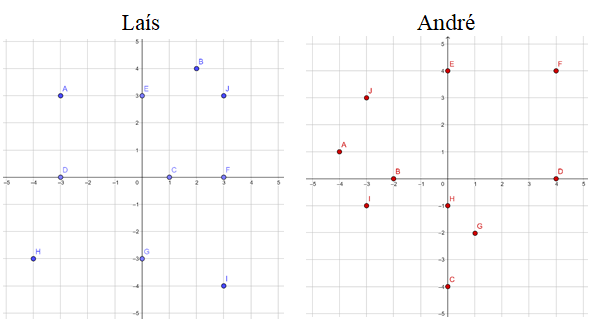
\includegraphics[width=375bp]{batalha.png}
\end{figure}

\begin{enumerate}
\item {}
	Laís é a primeira a jogar. Cite dois exemplos de equações-tiro que Laís pode dar para acertar pelo menos dois pontos marcados por André.

\item {}
	André, em sua jogada, usou $x^2 + y^2 = 9$ como equação-tiro. Qual a sua pontuação com essa jogada?

\item {}
	Dê exemplo de três equações-tiro que permitam à Laís acertar o ponto $A$ da cartela de André.

\item {}
	Suponha que Laís e André irão começar uma nova partida e que Laís inicie o jogo com a equação-tiro $x+2y = 4$. Dependendo dos pontos marcados por André em sua cartela, qual é a pontuação máxima que ela pode adquirir com essa jogada? Nesse caso, marque no plano cartesiano os pontos que ela terá acertado.

\item {}
	Com as regras que foram estabelecidas, existe alguma equação-tiro que André dê que acerte todos os pontos da cartela de Laís em uma única rodada?

\end{enumerate}

\end{task}


\clearpage
\def\currentcolor{session4}
\begin{texto}
{
  \subsection{Objetivo geral da seção}
  \begin{itemize}
  \item malizar a ideia de representar graficamente o conjunto solução de uma equação.
  \end{itemize}
  \subsection{Sugestões e discussões}

Aqui utilizaremos a representação gráfica de uma função para atribuir significado ao conjunto solução da equação.o. No texto nos fixamos no caso das funções do primeiro grau, mas o professor pode estender a conclusão para conjuntos do tipo $(x,f(x))$ ou para algum $(x,y)$ tais que $x$ e $y$ estejam relacionados em uma equação.

É importante que o professor deixe claro que o gráfico de uma função sempre representa o conjunto solução de uma equação (a saber, as equações do tipo $y=f(x)$), mas que nem sempre a representação gráfico do conjunto solução de uma equação é gráfico de uma função - como pode ser percebido no item $e)$ da atividade \hyperref[batalha-naval]{\textit{Batalha Naval}}. Já vimos também, por exemplo, a representação gráfica do conjunto solução da equação $x^2+y^2=25$ e vimos que essa representação não é gráfico de uma função, mas que há uma representação gráfica para esse conjunto de pontos independente de não ser uma função.
}
\end{texto}
\arrange{Equações: Siginificado Geométrico}
\label{\detokenize{AF107-1:organizando-taxa-de-variacao-media}}\label{\detokenize{AF107-1::doc}}


Nos capítulos anteriores deste livro de Funções, você aprendeu que em muitos casos, utilizamos expressões algébricas envolvendo uma variável para caracterizar funções definidas em conjuntos numéricos. Se considerarmos, por exemplo, a função $f: \mathbb{R} \to \mathbb{R}, \ f(x) = 2x+1$, a expressão $y=2x+1$ nos permite compreender como os elementos do domínio se relacionam com os do contradomínio, por exemplo, o número $3$ é associado ao número $7$, pois $f(3) = 2\cdot 3+1 = 7$. O gráfico desta função (uma reta) é a forma como representamos essa relação geometricamente. Ele é construído marcando os pontos $(x,y)$ do plano cartesiano tais que $y = f(x)$, isto é, $y = 2x+1$. Assim, a coleção de pontos do gráfico consiste exatamente de todos os pares de valores dados às variáveis $x$ e $y$ para os quais é verdadeira a igualdade $y = 2x + 1$, ou seja, são todas as soluções dessa equação.


\begin{figure}[H]
\centering

\noindent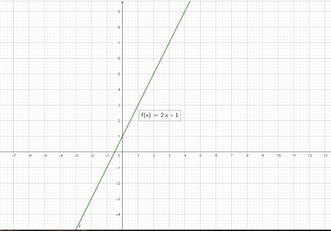
\includegraphics[width=200bp]{afim.png}
\end{figure}


Lembramos que uma equação é uma igualdade matemática envolvendo termos desconhecidos (em geral números reais) a serem determinados, por isso chamadas de \emph{incógnitas}. Uma \emph{solução} de uma equação que envolve apenas duas incógnitas $x$ e $y$ é um par ordenado de números reais $(a,b)$ tal que, uma vez convencionado que o primeiro termo do par ordenado refere-se à incógnita $x$ e o segundo à incógnita $y$, substituindo $x = a$ e $y = b$ nas expressões da equação, ainda obtemos uma afirmação verdadeira. Como exemplo, o par $(2,3)$ é uma solução da equação $y = 2x-1$. O conjunto de todas as soluções de uma equação em duas incógnitas é denominado \emph{conjunto solução} ou \emph{solução geral} desta equação.

De maneira geral, quando temos uma equação em duas incógnitas $x$ e $y$, mesmo que seu conjunto solução não represente o gráfico de uma função, podemos representar graficamente a sua solução geral no plano cartesiano, analisando-as de uma maneira mais visual, através de um desenho neste plano, o que pode nos ajudar a entender melhor certos padrões dessas soluções. Por exemplo, pode-se mostrar que a solução geral da equação $x^2+y^2=25$ forma o desenho de uma circunferência de raio 5 no plano, com centro na origem. Você deve ter percebido isso na atividade \hyperref[castelo]{\textit{Enigma do Castelo}}. Observando esta figura, pode-se concluir que se o par $(x,y)$ é solução desta equação, então os valores de $x$ e de $y$ devem estar, cada um, no intervalo $[-5,5]$.

\begin{figure}[H]
\centering

\noindent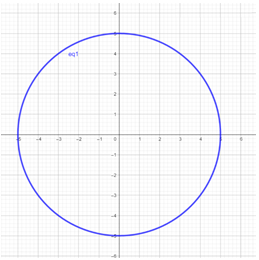
\includegraphics[width=200bp]{circulo.png}
\end{figure}

Esta perspectiva de estudo das soluções de equações de duas variáveis por meio do plano cartesiano foi desenvolvida pelo matemático René Descartes (1596-1650). Em seu livro Discours de la méthode, que teve sua primeira edição publicada em 1637, ele propôs uma nova perspectiva de estudo da Geometria e da Álgebra. Desde a antiguidade até o século XVII, os objetos da Geometria eram caracterizados apenas por descrições dos lugares geométricos das figuras planas e por construções geométricas. Por exemplo, uma circunferência era definida somente como o lugar geométrico dos pontos que têm mesma distância a um certo ponto O fixado, denominado centro da circunferência.

 A partir da abordagem sugerida por Descartes, tornou-se possível conceber alguns objetos geométricos como curvas no plano cartesiano que passam a ser descritas por equações cujas soluções são os todos os pontos que pertencem a essa curva. Por exemplo, um círculo de raio $r$ e centro na origem $O = (0,0)$ é caracterizado pelo conjunto de pontos $(x,y)$ que são soluções da equação $x^2+y^2 = r^2$. Repare que, ao fazermos $r =5$, obtemos exatamente a equação e a circunferência estudadas na atividade \hyperref[castelo]{\textit{Enigma do Castelo}}.

\begin{figure}[H]
\centering

\noindent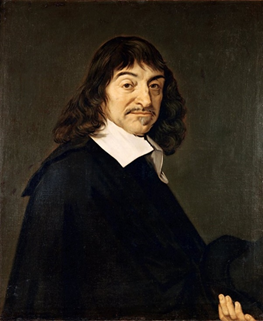
\includegraphics[width=150bp]{descartes.png}
\end{figure}

Desse modo, Descartes estabeleceu uma interligação entre a Geometria e a Álgebra hoje conhecida como Geometria Analítica, com o intuito de utilizar as vantagens de uma área para complementar a outra. Como a Geometria é muito visual e intuitiva, podemos por vezes ser enganados pelos olhos e chegar a conclusões incorretas; por outro lado, com seus símbolos e equações, a Álgebra é uma ferramenta poderosa para modelar e resolver problemas, mas em algumas vezes, seu excesso de símbolos pode confundir e nos levar a erros. Desta união, surge a Geometria Analítica, área da Matemática que visa representar e estudar objetos da Geometria através do estudo de soluções de equações e vice-versa.
Nas figuras abaixo ilustramos alguns exemplos de equações em duas variáveis e da representação gráfica das suas soluções gerais, todas plotadas com o auxílio do \emph{software} GeoGebra:

\begin{figure}[H]
\centering

\noindent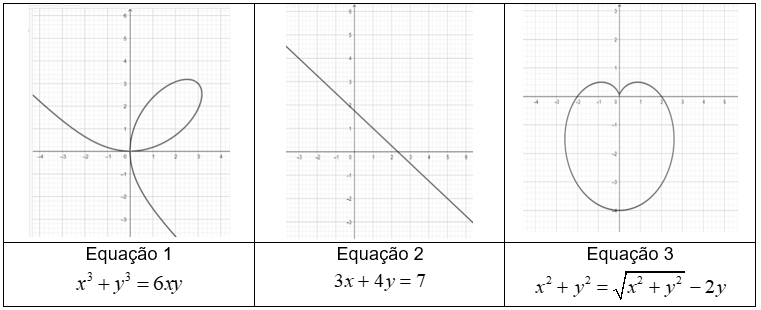
\includegraphics[width=300bp]{ga.png}
\end{figure}


\begin{reflection}

Junto com os seus colegas, reveja os exemplos de equações em duas variáveis estudadas até aqui e da representação gráfica das suas soluções gerais. Está certo afirmar que todos eles representam gráficos de funções? Por quê? Existe algum critério para determinar se a representação gráfica da solução geral de uma equação é o gráfico de uma função?

\end{reflection}


\clearpage
\def\currentcolor{session2}
\begin{objectives}{Estádio de Futebol}
{
\begin{itemize}
\item Apresentar a possibilidade de outros tipos de equações.
\item Familiarizar o aluno com a ideia de que curvas no plano podem ser representadas algebricamente por equações, e vice-versa.
\item Usar o Geogebra para resgatar a ideia de sistemas de equações
\end{itemize}
}{1}{2}
\end{objectives}
\marginpar{\vspace{-2.5em}}
\begin{sugestions}{Estádio de Futebol}
{
\begin{itemize}
\item  Nessa atividade, vamos acrescentar mais um conjunto solução de uma classe bem específica de equações: a equação de uma elipse mas é apenas a título de exemplo
\item O objetivo é que o aluno se familiarize com a ideia de que curvas no plano podem ser representadas algebricamente por equações, e vice-versa - mas não nos aprofundaremos muito em modelos de equação que não sejam as equações polinomiais do primeiro e segundo graus.
\item Problematize junto aos alunos o motivo do centro do campo estar associado à origem do sistema cartesiano. Auxilie-os a perceber que a curva a que nos referimos - no caso, o contorno do Mineirão - seria a mesma em qualquer posição dentro do sistema de eixos cartesianos, com os eixos contendo seus pontos máximos  ou não, mas que essas configurações não são interessantes porque as equações assim geradas seriam bem mais complexas.
Essa situação pode ser experimentada da seguinte maneira: Abra uma tela do GeoGebra, cole a imagem do Mineirão e rotacione. Tome 5 pontos no contorno mais externo da imagem do estádio e gere a cônica que passa por esses 5 pontos. Por exemplo:
{\footnotesize https://www.geogebra.org/classic/ujwf9gdx}  
\item Nos itens \titem{a)} e \titem{b)}, o professor deve ajudar o aluno a perceber que os pontos dos eixos $x$ e $y$ obedecem às equações $y=0$  e $x=0$, respectivamente.
\item No item \titem{c)}, a proposta é que o aluno busque livremente esses valores, da mesma forma que realizado com o \hyperref[castelo]{\textit{Enigma do Castelo}}.
\end{itemize}
}{1}{2}
\end{sugestions}
\marginpar{\vspace{-1.5em}}
\begin{answer}{Estádio de Futebol}
{
\begin{enumerate}
\item $8.$
\item $3.$
\item Não. Faça os alunos perceberem que os valores de $x$ variam entre $-4$ e $4$, que os valores de $y$ variam entre $-3$ e $3$ e testarem os candidatos vendo que não satisfazem a equação.
\end{enumerate}
}{1}
\end{answer}
\clearmargin
\begin{objectives}{Fábrica de bolo}
{
\begin{itemize}
\item Levar o aluno a desenvolver a capacidade de modelar fenômenos reais por meio de equações lineares de duas variáveis.
\item Encontrar soluções condizentes com a realidade (o aluno deve ser capaz de saber que, nesse problema, só são admitidas soluções inteiras positivas
\end{itemize}
}{1}{1}
\end{objectives}
\begin{sugestions}{Fábrica de bolo}
{
\begin{itemize}
\item A abordagem a essa questão pode começar com tentativa  e erro e depois, com a condução do profesor, o aluno pode chegar a equação $15f+18c=684$ que relaciona as quantidades de bolos vendidos, onde $c$ representa a quantidade de bolos de chocolate e $f$ os de fubá;.
\item Aproveite as diferentes respostas que os estudantes poderão encontrar. Todas elas estão corretas? Existiria mais de uma resposta correta? Note que esta última questão admite uma discussão numérica:
$f=\frac{684-18c}{15}$ é inteiro. O numerador é múltiplo de $3$ pois $684$ e $18$ o são, logo, temos que $684 -18c$ é múltiplo de 5. Segue que $684-18c$ deve terminar em $0$ ou em $5$, o que equivale a dizer que $18c$ deve terminar em $4$ ou em $9$. Como $18c$ é par,  isso equivale a dizer que $18c$ deve terminar em $4$, isto é, $c$ termina com $3$ ou $8$. Isso possibilita refinar e determinar rapidamente as possibilidades de soluções inteiras: $c = 3, 8, 13, 18, 23, 28, 33, 38.$
\end{itemize}
}{1}{1}
\end{sugestions}
\begin{answer}{Fábrica de bolo}
{
\begin{enumerate}
\item Denotando as possibilidades por pares do tipo $(c,f)$, onde $c$ é a quantidade de bolos de chocolate e $f$ a de fubá, temos as seguintes possibilidades $(3,42), (8,36), (13,30), \newline (18,24), (23,18), (28,12), \newline(33,6),(38,0)$;
\item Atividade exploratória.
\item Não, pois essa venda renderia R\$ $900{,}00$, o que excede os vencimentos do dia.
\end{enumerate}
}{1}
\end{answer}

\practice{Equações: Significado Geométrico}
\label{\detokenize{AF107-1:praticando-taxa-de-variacao-media}}\label{\detokenize{AF107-1::doc}}

\begin{task}{Estádio de Futebol}
\label{estadio}

O Estádio Governador Magalhães Pinto, mais conhecido como Mineirão, é um estádio de futebol localizado em Belo Horizonte, capital de Minas Gerais. Na \fref{mineirao}, pode-se ver uma foto da vista aérea do estádio através do \emph{Google Earth}. O contorno externo do estádio, realçado na figura por uma linha azul, é aproximado por uma elipse. Suponha que tenham sido introduzidas coordenadas cartesianas e unidades de medida de comprimento nesta foto. A origem $O$ foi escolhida para ser o centro do campo de futebol e os pontos $(x, y)$ do contorno externo do estádio são exatamente aqueles que são soluções da equação $9x^2 = 144 - 16y^2$.



\begin{figure}[H]
\centering

\noindent\includegraphics[width=300bp]{mineirao_com_eixos.png}
\caption{Estádio do Mineirão com os eixos marcados}
\label{mineirao}
\end{figure}

\begin{enumerate}

\item{} 
Qual a distância entre os pontos do contorno externo do Mineirão que estão sobre o eixo $x$?

\item{}
Qual a distância do centro do campo de futebol a qualquer um dos dois pontos do contorno externo do estádio que estão sobre o eixo $y$?

\item{}
Existe algum ponto $(a,b)$ do contorno externo do Mineirão que não esteja sobre os eixos coordenados de modo que $a$ e $b$ sejam números inteiros? Justifique.


\end{enumerate}

\end{task}

\clearpage
\begin{task}{Fábrica de Bolos}
\label{bolos}


A fábrica de bolos “Tia Tatá”{} produz e vende bolos de diversos tipos, mas os mais solicitados são o de fubá e o de chocolate, que custam $15$ reais e $18$ reais cada um, respectivamente. Em um determinado dia, a venda dos bolos de fubá e de chocolate gerou $684$ reais em caixa.

\begin{enumerate}

\item{}
Quantos bolos de cada tipo podem ter sido vendidos nesse dia?

\item{}
Use a construção no GeoGebra disponível em \url{https://www.geogebra.org/classic/juvucjuh}, para movimentar o controle deslizante $k$ e checar a sua resposta dada no item \titem{a)}. Diga como você pode usar essa ferramenta para encontrar outras respostas para o item \titem{a)}.

\item{}
Seria possível que a venda de bolos de chocolate nesse dia fosse de $50$ bolos? Justifique.
\end{enumerate}
\end{task}


\cleardoublepage
\def\currentcolor{session1}
\begin{objectives}{Faturamento de um Teatro}
{
\begin{itemize}
\item Introduzir equações com 3 incógnitas
\item trabalhar com um sistema de equações, explorando o fato de que, quando ele tem solução não-vazia, essa solução pode não ser única.
\item Observar o fato de que acrescentando outras equações ao sistema, se restringe o número de soluções.
\end{itemize}
}{1}{1}
\end{objectives}
\begin{sugestions}{Faturamento de um Teatro}
{
\begin{itemize}
\item No item \titem{a)} ajude seus alunos a analisar quais são as variáveis que influenciam na relação entre o faturamento e a quantidade de expectadores, de acordo com o seu perfil. 
\item Em \titem{b)} você deve estimular seus alunos a atribuir valores e pesquisar soluções, considerando as restrições de que precisamos ter variáveis que sejam números inteiros positivos. 
\item Em \titem{c)} estamos restringindo o conjunto das soluções, criando uma relação entre duas das variáveis envolvidas. Ajude seus alunos a estabelecer essa relação e a considera-la em conjunto com o que foi registrado no item \titem{a)}
\end{itemize}
}{1}{1}
\end{sugestions}
\begin{answer}{Faturamento de um Teatro}
{
\begin{enumerate}
\item Sejam $x,y$ e $z$ a quantidade de inteiras, meias e gratuidades, respectivamente, $x+y+z=500$ e $50x+25y=20500.$
\item Atividade exploratória, mas o professor pode pensar na solução da equação $50x+25y=20500$ considerando a restrição $x+y<500$.
\item $(350,120)$
\end{enumerate}
}{1}
\end{answer}
\begin{objectives}{Retornando ao Estádio Mineirão}
{
\begin{itemize}
\item Trabalhar a intercessão entre os  conjuntos solução de uma equação da elipse e uma equação linear
\end{itemize}
}{1}{1}
\end{objectives}
\clearmargin
\begin{sugestions}{Retornando ao Estádio Mineirão}
{
\begin{itemize}
\item No item \titem{a)}, é interessante que o aluno esboce a figura, de forma a verificar possíveis interseções. Auxilie-o a perceber que os pontos de interseção entre a reta e as elipses são pontos que pertencem tanto á reta quanto a cada elipse, sendo portanto soluções que satisfazem aos pares respectivos de reta e elipse. Além disso, o aluno precisará considerar ainda uma direção estabelecida, que implica na busca das interseções que estejam no segundo quadrante.
\item No item  \titem{b)}, a situação é análoga à de \titem{a}), mas em lugar de termos a reta que modela o chute, temos a direção estabelecida por dois pontos: o centro e o ponto $(1,1)$. Caberá ao aluno determinar qual seria a equação dessa reta, o que pode ser feito considerando seus conhecimentos sobre funções afins, e a seguir, atuar conforme feito no item \titem{a)}.
\end{itemize}
}{1}{2}
\end{sugestions}
\begin{answer}{Retornando ao Estádio Mineirão}
{
\begin{enumerate}
\item $\displaystyle eq_1:(-\frac{12}{5},\frac{12}{5} );\ \newline eq_2:(-\frac{2\sqrt{5}}{5},\frac{2\sqrt{5}}{5});\  \newline eq_3:(-\frac{6\sqrt{13}}{13},\frac{6\sqrt{13}}{13})$
\item $\displaystyle eq_1:(\frac{12}{5},\frac{12}{5} );\ \newline eq_2:(\frac{2\sqrt{5}}{5},\frac{2\sqrt{5}}{5});\  \newline eq_3:(\frac{6\sqrt{13}}{13},\frac{6\sqrt{13}}{13})$
\end{enumerate}
}{1}
\end{answer}
\explore{Sistemas de Equações}
\label{\detokenize{AF107-2:explorando-sistemas-de-equações}}\label{\detokenize{AF107-2::doc}}

\begin{task}{Faturamento de um Teatro}
\label{teatro}

Um teatro conta com 500 assentos. Uma peça que está fazendo muito sucesso entrou em cartaz nesse teatro e, em uma determinada noite de apresentação, todos os ingressos foram vendidos, obtendo um faturamento de R\$ $20.500{,}00$ com a bilheteria. A entrada cheia nesse teatro custa R\$ $50{,}00$, sendo que pessoas com mais de 65 anos pagam meia entrada e os aniversariantes têm gratuidade.

\begin{figure}[H]
\centering

\noindent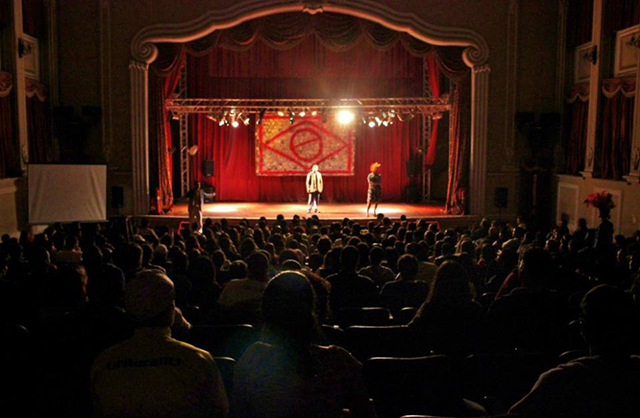
\includegraphics[width=175bp]{teatro.png}
\end{figure}
\begin{enumerate}

\item{}
Escreva duas equações que modelem as informações do enunciado. Quantas variáveis você necessita dispor para isso?

\item{}
Encontre três possibilidades para o número de ingressos vendidos de entrada cheia, meia entrada e de gratuidade que poderiam ter ocorrido, com as condições informadas no enunciado.

\item{}
Suponha que na noite do espetáculo, o número de pessoas com mais de 65 anos foi quatro vezes o número de aniversariantes. Quantos aniversariantes estiveram na plateia nesse dia?

\end{enumerate}

\end{task}

\begin{task}{Retornando ao Estádio do Mineirão}
\label{estadio2}

Manoel Rezende de Mattos Cabral, mais conhecido como Nelinho, foi um jogador de futebol brasileiro que atuava como lateral direito e participou como titular da seleção brasileira nas copas de 1974 e 1978. Em 1979, ao ser desafiado por uma emissora de televisão, Nelinho conseguiu chutar uma bola para fora do estádio do Mineirão, estando dentro do campo (veja a façanha de Nelinho em \url{https://www.youtube.com/watch?v=psJJEdZHpcU}).


Na Atividade \hyperref[estadio]{Estádio de Futebol} da seção anterior, consideramos que o Estádio do Mineirão pode ter o seu contorno externo representado por uma elipse de equação $9x^2 = 144 - 16y^2$, em um sistema de coordenadas cartesianas, conforme indicado na figura a seguir, com o centro do campo coincidindo com a origem $(0,0)$ e de forma que as unidades de medida reais estejam em escala com este sistema.

\begin{figure}[H]
\centering

\noindent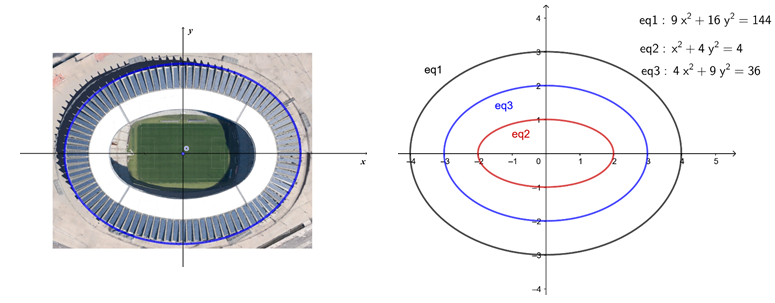
\includegraphics[width=350bp]{estadio2.png}
\end{figure}
\begin{enumerate} 

\item{}
Assumindo uma vista aérea conforme representada nas figuras anteriores, suponha que Nelinho tenha chutado a bola a partir do centro do campo em direção ao corner do time adversário (2\super{o} quadrante) em trajetória retilínea (numa vista aérea) que segue a equação $y = -x$. Em que pontos do plano cartesiano a projeção da trajetória dessa bola cruzará as três elipses?

\item{}
Novamente, Nelinho está no centro do campo de jogo e deu um outro chute, agora na direção do ponto $(1,1)$, de forma que, numa vista aérea, a bola segue uma trajetória retilínea e sai do estádio. Em que pontos (no primeiro quadrante) a vista aérea desse chute intersecta as três elipses?

\end{enumerate}
\end{task}


\arrange{Sistemas de Equações}
\label{\detokenize{AF107-2:organizando-sistemas-de-equações}}\label{\detokenize{AF107-2::doc}}

Nas atividades anteriores, você percebeu que as equações e suas respectivas soluções podem representar matematicamente situações de um determinado contexto. Determinados casos podem exigir o uso equações simultâneas, como ilustrado nas atividades \hyperref[teatro]{\textit{Faturamento de um Teatro}} e \hyperref[estadio2]{\textit{Retornando ao estádio do Mineirão}}. Um conjunto finito de equações consideradas simultaneamente em um problema é chamado um \emph{sistema de equações} ou simplesmente um \emph{sistema}. Assim, no contexto do item \titem{b)} da atividade ), as equações $9x^2 = 144 - 16y^2$ e $y = -x$ compõem um sistema de duas equações. É usual organizar um sistema de equações listando-as uma abaixo da outra à direita de um símbolo de chave que engloba todas as equações , como ilustrado abaixo:

\begin{equation*}
\left\{
\begin{aligned}
9x^2&=144-16y^2\\
y&=-x
\end{aligned}
\right.
\end{equation*}

As incógnitas que aparecem em, pelo menos uma das equações são chamadas de \emph{incógnitas do sistema de equações}. As incógnitas do sistema do exemplo acima são $x$ e $y$.
 
Uma \emph{solução} de um sistema de $m$ equações e $n$ incógnitas é um conjunto ordenado de valores para as $n$ incógnitas que satisfazem às m equações simultaneamente.  Mais precisamente, se um sistema de equações tem $n$ incógnitas, digamos $x_1, x_2, \ldots, x_n$ uma solução do sistema é uma lista ordenada de números reais $(a_1, a_2, \ldots, a_n)$tais que ao fazer $x_1 = a_1 , x_2 = a_2, \ldots, x_n = a_n$ obtemos uma solução para todas as equações do sistema. Em particular, se um sistema tem apenas 2 incógnitas $x$ e $y$, então as soluções desse sistema serão pares ordenados $(a,b$), ou seja, pontos do plano cartesiano.

Quando o sistema de equações tem apenas duas incógnitas, as suas soluções têm uma interpretação geométrica no plano cartesiano $\mathbb{R}^2$. De fato, conforme vimos nas seções anteriores, algumas curvas no $\mathbb{R}^2$ são a representação geométrica do conjunto solução de uma equação. Considerando a equação $y^2 + x^2 = 3$, podemos destacar os pontos $(1, \sqrt{2})$, $(1, - \sqrt{2})$ e $(\frac{\sqrt{11}}{2}, \frac{1}{2})$ como exemplos de soluções da mesma (há infinitas soluções para essa equação! Por quê?). Observe que o ponto $A = (1, \sqrt{2})$ também pertence ao conjunto solução da equação $y - x\cdot \sqrt{2} = 0$ e ainda da equação $y - x^2 = -1 + \sqrt{2}$ ou da equação $x + y = 1 + \sqrt{2}$ assim como de muitas outras!

 Assim, vemos que o ponto $A = (1, \sqrt{2})$ é uma solução do seguinte sistema:

\begin{equation*}
\left\{
\begin{aligned}
y^2+x^2&=3\\
y-x\cdot\sqrt{2}&=0\\
y-x^2&=-1+\sqrt{2}\\
x+y&=1+\sqrt{2}
\end{aligned}
\right.
\end{equation*}

Geometricamente, podemos dizer então que o ponto $A$ está na interseção entre as curvas $y^2 + x^2 = 3$  , $y - x\cdot \sqrt{2} = 0$ ,  $y - x^2 = -1 + \sqrt{2}$ e ainda $x + y = 1 + \sqrt{2}$. Veja a figura abaixo, onde plotamos essas curvas no \emph{software} GeoGebra: 


\begin{figure}[H]
\centering

\noindent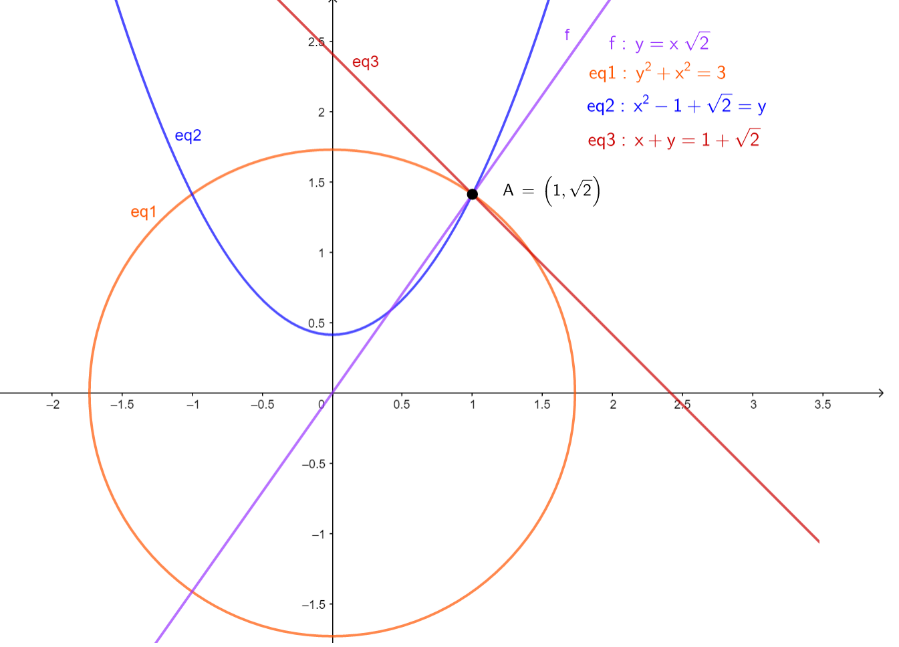
\includegraphics[width=300bp]{curvas.png}
\end{figure}


Então, quando um mesmo ponto $(a,b)$ satisfaz a duas ou mais equações ao mesmo tempo, temos que esse ponto pertence ao conjunto solução dessas equações, assim, ao representarmos geometricamente esses conjuntos, esse ponto estará em todas essas curvas, portanto, estará na interseção entre elas.

Nem sempre curvas representadas em um mesmo sistema de eixos apresentam pontos de interseção. A figura a seguir fornece um exemplo de 4 curvas correspondendo às soluções das equações $x^2 + y^2 = 3$, $x^2 + y^2 = 2$, $x^2 - y = -2$ e $x+y = -3$. O conjunto solução do sistema de equações formado por essas 4 equações é vazio, pois não há um ponto que pertença simultaneamente a todas as curvas.


\begin{figure}[H]
\centering

\noindent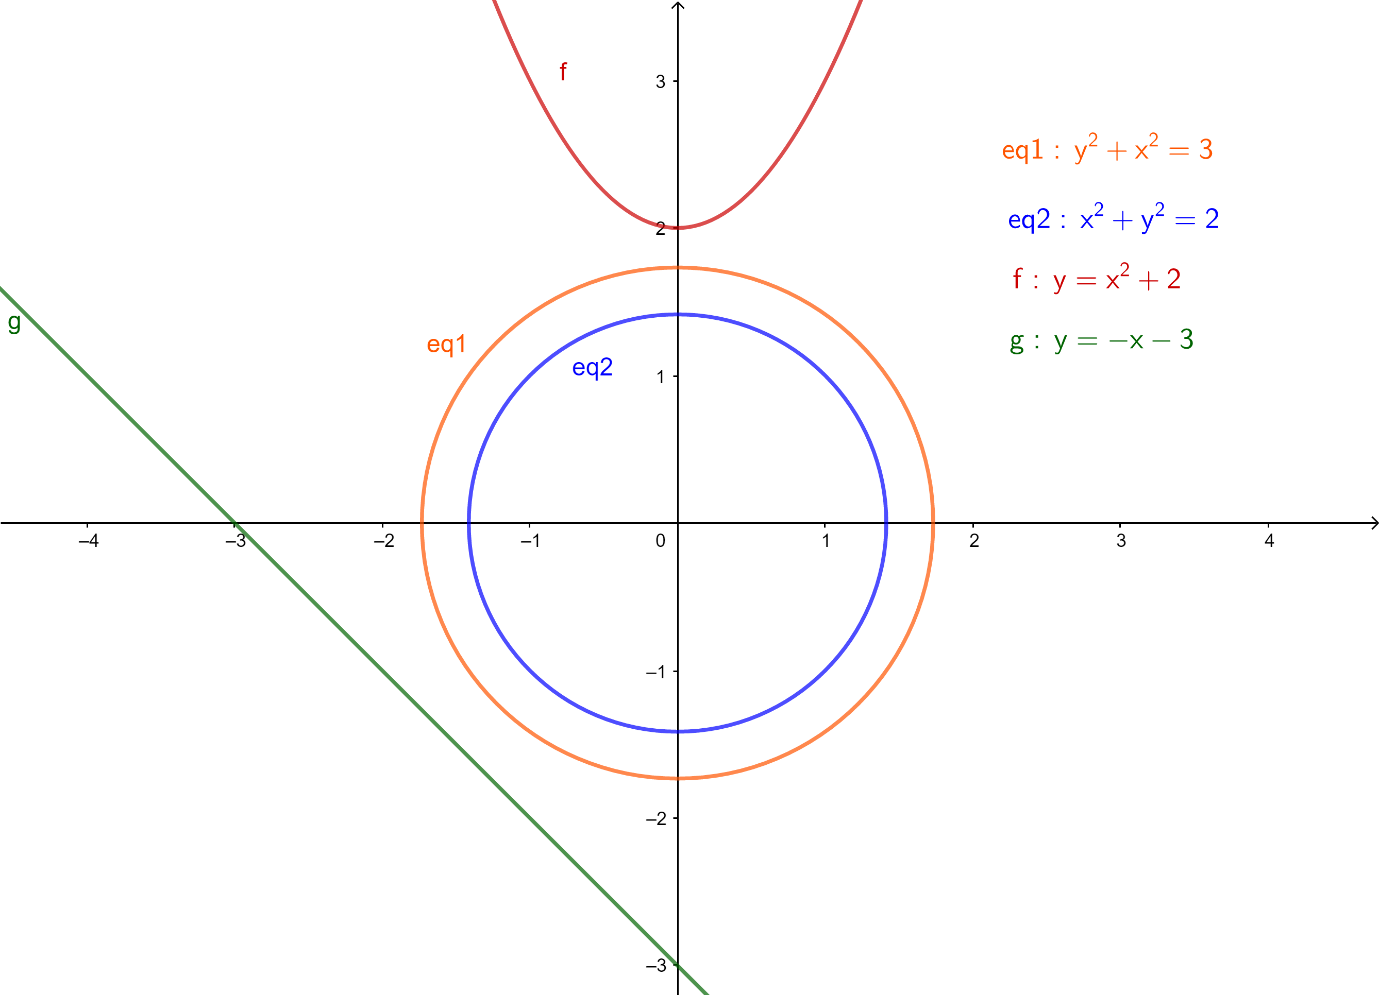
\includegraphics[width=300bp]{curvassemintersecao.png}
\end{figure}


\textbf{Exemplo:} Considere a seguinte lista de 5 equações em duas incógnitas: $y = x \cdot \sqrt{2}$, \ $y -x^2 = -1 + \sqrt{2}$, \ $ x+y = 1 + \sqrt{2}$, \ $y^2 + x^2 = 3$ e $y-x = -1$. O conjunto solução de cada uma dessas equações está descrito geometricamente na figura abaixo.  

\clearmargin
\def\currentcolor{session2}
\begin{objectives}{Construindo Sistemas}
{
\begin{itemize}
\item Fazer o aluno propor problemas.
\item Relacionar intercessões de curvas com soluções de sistemas. 
\end{itemize}
}{1}{1}
\end{objectives}
\marginpar{\vspace{-2em}}
\begin{sugestions}{Construindo Sistemas}
{
Nessa atividade, faça o aluno entender a relação entra as curvas e suas respectivas equações e consolidar a ideia que a intercessão entre as curvas (quando existente) correspondem às soluções dos sistemas constituídos por essas equações. 
}{1}{1}
\end{sugestions}
\begin{answer}{Construindo Sistemas}
{
\begin{enumerate}
\item Basta tomar um conjunto de três equações que não tenham um ponto em comum a todas simultaneamente. Por exemplo, o sistema formado por $f, g$ e $h$.
\item O sistema composto pelas equações $f$ e $g$ e o sistema formado por $eq_1$ e $eq_2$.
\end{enumerate}
}{0}
\end{answer}
\begin{objectives}{Praticando Sistemas de Equações no Geogebra}
{
\begin{itemize}
\item Explorar o Geogebra como ferramenta para estudo de sistemas.
\item Classificar os sistemas em função de seu conjunto solução. 
\end{itemize}
}{1}{1}
\end{objectives}
\marginpar{\vspace{-2em}}
\begin{sugestions}{Praticando Sistemas de Equações no Geogebra}
{
\begin{itemize}
\item Essa atividade foi pensada para ser realizada com o apoio do GeoGebra. São, portanto, sugestões de construções que poderão contribuir para que o aluno compreenda a ideia da solução de um sistema linear, além de sugerir ao estudante que  um sistema pode ser possível e determinado, possível e indeterminado ou impossível.
\item No item $c)$ convém buscar junto aos alunos que estratégias adotariam para escrever esses sistemas. Por exemplo, o estudante pode, usando o GeoGebra, traçar duas retas quaisquer que passem por $(1,1)$ e registrar o sistema formado por essas duas retas ou ainda, algebricamente, pode tomar expressões como $x + 2y$ e $3x-y$, por exemplo, substituindo os valores $x=1$ e $y=1$ em cada uma dela.
\end{itemize}
}{1}{1}
\end{sugestions}
\begin{answer}{Praticando Sistemas de Equações no Geogebra}
{
\begin{enumerate}
\item Retas.
\item Para que o sistema tenha infinitas soluções, os valores para $a, b$ e $c$ deverão ser os mesmos associados à equação $x-2y=8$, ou seja, $a=1, b=-2$ e $c=8$. Não é possível que o sistema tenha duas soluções, pois não é possível que duas retas tenham exatamente  dois pontos em comum. Uma única solução será encontrada para $a\neq 1$ ou $b \neq -2$ ou $c \neq 8$. Cabe observar que para $c \neq 8$, se $a$ e $b$ forem respectivamente iguais a $1$ e $-2$, então o sistema não terá solução.
\item $(2,-3)$ é solução da equação $1$. Há infinitos valores para $a, b$ e $c$ para os quais a reta dada pela equação $2$ passará por $(2,-3)$, entre eles, $a=1, b=1$ e $c=-1$.
\item $x+2y=3$ e $3x-y=2$, formando um sistema.
\end{enumerate}
}{0}
\end{answer}

\def\currentcolor{session4}

\begin{figure}[H]
\centering

\noindent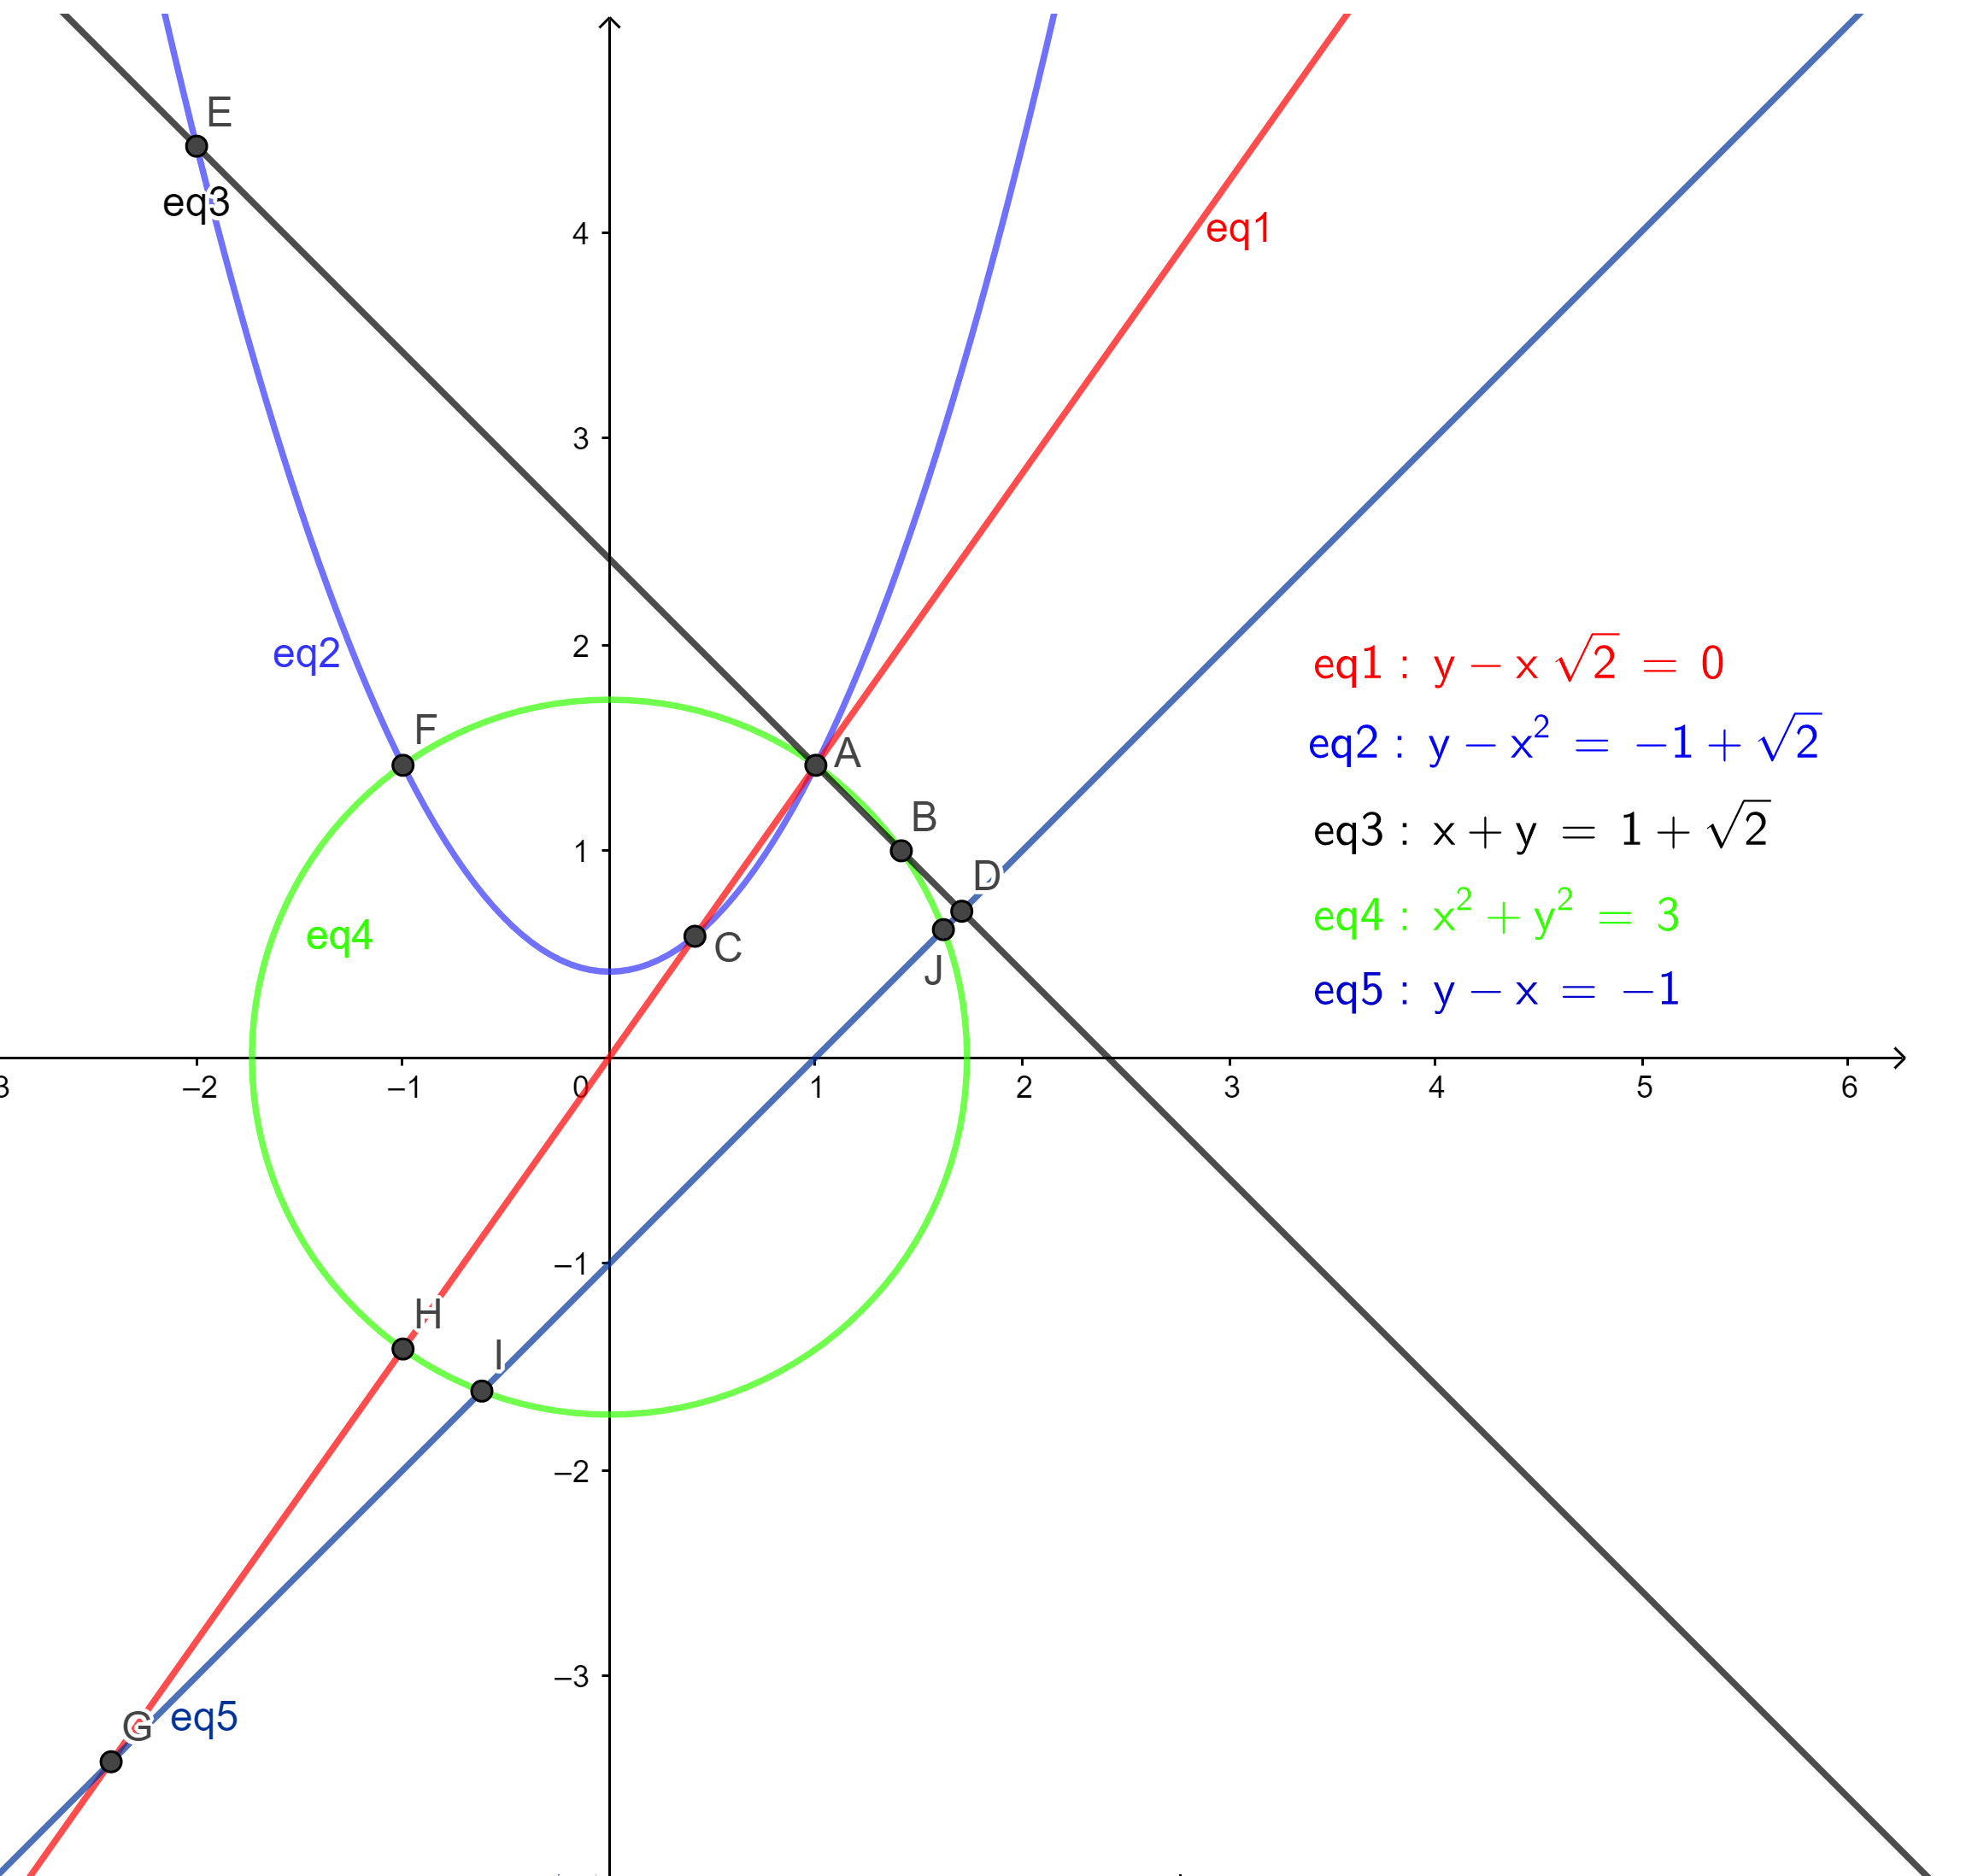
\includegraphics[width=300bp]{exemplo_sistemas.png}
\end{figure}

Considere os três sistemas \titem{(I)}, \titem{(II)} e \titem{(III)} abaixo, todos compostos por equações dessa lista:



\begin{enumerate}[label=\titem{(\Roman*)}]
\small
\begin{minipage}{.33\linewidth}
\null\vfill
\item 
$
\left\{
\begin{aligned}
y-x\cdot\sqrt{2}&=0\\
y-x^2&=-1+\sqrt{2}\\
x+2&=1+\sqrt{2}
\end{aligned}
\right.
$
\vfill\null
\end{minipage}
\begin{minipage}{.33\linewidth}
\null\vfill
\item 
$
\left\{
\begin{aligned}
y^2+x^2&=3\\
x+y&=1+\sqrt{2}
\end{aligned}
\right.
$
\vfill\null
\end{minipage}
\begin{minipage}{.33\linewidth}
\null\vfill
\item 
$
\left\{
\begin{aligned}
y-x\cdot\sqrt{2}&=0\\
y-x^2&=-1+\sqrt{2}
\end{aligned}
\right.
$
\vfill\null
\end{minipage}
\end{enumerate}

\needspace{5em}
Analisando a última figura, podemos concluir que:

\begin{enumerate}
\item O sistema \titem{(I)} possui tem única solução, dada pelo ponto $A$. 

\item O sistema \titem{(II)} possui duas soluções, dadas pelos pontos $A$ e $B$. 

\item O sistema \titem{(III)} possui duas soluções, dadas pelos pontos $A$ e $C$.

\item O sistema dado pelas cinco equações da lista dada neste exemplo tem solução vazia, visto que não há um ponto que pertença simultaneamente às $5$ curvas da figura acima.
\end{enumerate}


  

\practice{Sistemas de Equações}
\label{\detokenize{AF107-2:praticando-sistemas-de-equaçoes}}\label{\detokenize{AF107-2::doc}}

\begin{task}{Construindo Sistemas}

Utilizando apenas equações que aparecem na figura do último exemplo, construa sistemas de equações com as propriedades pedidas abaixo, indicando na figura quais os pontos que correspondem às suas respectivas soluções.

\begin{enumerate}
\item{}
Um sistema com três equações da figura que não possua solução;

\item{}
Dois sistemas que tenham exatamente duas soluções;


\end{enumerate}



\end{task}


\begin{task}{Praticando Sistemas de Equações no GeoGebra}

Abra o GeoGebra no seu \emph{smartphone}, no aplicativo calculadora gráfica. No campo de entrada, digite as equações $x - 2y = 8$ (Equação 1) e em seguida, $ax+ by = c$ (Equação 2). O GeoGebra irá criar controles deslizantes para os coeficientes a, b e c da Equação 2. Nos itens a seguir, considere o sistema formado pelas equações 1 e 2 nas incógnitas $x$ e $y$.

\begin{enumerate}
\item{} 
Qual figura está associada ao conjunto solução da Equação 1? E da Equação 2?

\item{}
Existem valores para os coeficientes $a$, $b$ e $c$ de forma que o sistema formando pelas Equações 1 e 2 possua uma única solução? E apenas duas soluções? E infinitas soluções?

\item{}
Insira o ponto $(2,-3)$ no campo de entrada. Ele é uma solução da Equação 1 (por quê?). Usando os controles deslizantes, obtenha valores para os coeficientes a, b e c de forma que esse ponto seja solução do sistema.

\item{}
Elabore um sistema com duas equações diferentes que tenha o ponto $(1, 1)$ como única solução. Construa as curvas correspondentes a essas equações no GeoGebra para realizar uma "prova real"{} do sistema que você elaborou.
\end{enumerate}

\end{task}
\cleardoublepage
\def\currentcolor{session1}
\begin{objectives}{Clube de Esportes}
{
\begin{itemize}
\item Estudar algebricamente a resolução de sistemas a partir de determinados contextos.
\end{itemize}
}{1}{1}
\end{objectives}
\begin{sugestions}{Clube de Esportes}
{
\begin{itemize}
\item No item \titem{a)} conduza o raciocínio do aluno da seguinte maneira "Se o clube tem $120$ adultos associados, então arrecadou-se $120 \times 6 = 720$ reais com os adultos. Para o total de $1000$ reais, restam $280$ reais. Como cada criança entrou com $4$ reais, temos $280/4=70$ crianças".
\item No item \titem{b)} conduza um raciocínio análogo ao do item \titem{a)}.
\end{itemize}
}{1}{1}
\end{sugestions}
\begin{answer}{Clube de Esportes}
{
\begin{enumerate}
\item $70$ crianças.
\item $60$ adultos.
\item 
\adjustbox{valign=t}
{
\begin{tabular}{|>$e{.25\linewidth}<$|>$e{.25\linewidth}<$|>$e{.25\linewidth}<$|}
\hline
$\tcolor{N\super{o} de crianças associadas}$ & $\tcolor{N\super{o} de adultos associados}$ & \tmat{(x,y)} \tabularnewline
\hline
40 & 140 & (40,140) \tabularnewline
\hline
205 & 30 & (205,30) \tabularnewline
\hline
25 & 150 & (25,150) \tabularnewline
\hline
100 & 100 & (100,100) \tabularnewline
\hline
x & \dfrac{1000-4x}{6} & \bigg(x,\dfrac{1000-4x}{6}\bigg) \tabularnewline
\hline
\dfrac{1000-6y}{4} & y & \bigg(\dfrac{100-6y}{4},y\bigg) \tabularnewline
\hline
\end{tabular}
}
\item $4x+6y=1000$
\end{enumerate}
}{1}
\end{answer}

\explore{Equações Lineares em 2 Incógnitas}
\label{\detokenize{AF107-3:explorando-equaçoes-lineares-2-incognitas}}\label{\detokenize{AF107-3::doc}}
\vspace{-2\parskip}
\vspace{-1em}
\phantom{M}
\begin{task}{Clube de Esportes}
\label{clube}


Um clube precisa realizar uma reforma na sua piscina, e para isso, cobrará uma taxa de cada associado. Cada adulto pagará R\$ $6{,}00$ reais e cada criança R\$ $4{,}00$. 

\begin{figure}[H]
\centering

\noindent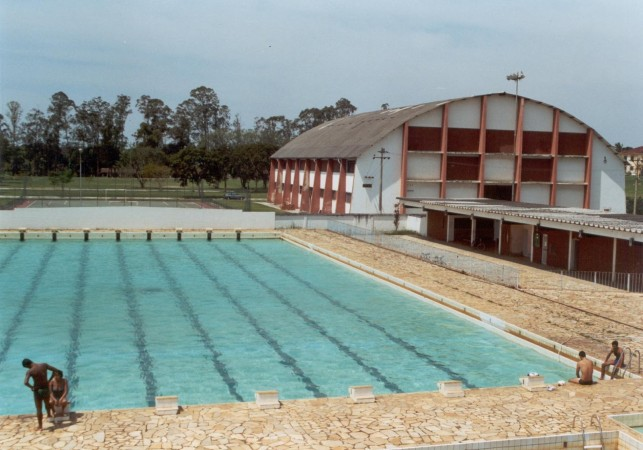
\includegraphics[width=265bp]{piscina.jpg}
\end{figure}


Sabendo que a obra está orçada em R\$ $1000{,}00$ e que o valor arrecadado foi exatamente o do preço da obra, responda:

\begin{enumerate}

\item{}
Se o clube tem $120$ adultos associados, quantos associados são crianças?

\item{}
Se forem $160$ crianças associadas, quantos serão os adultos?

\item{} 
Complete a tabela a seguir em termos de $x$ e $y$, gerando pares ordenados com essas variáveis, usando $x$ para representar o número de crianças e $y$ para representar o número de adultos.


\begin{table}[H]
\centering
\begin{tabular}{|c|c|c|}
\hline
\tcolor{N\super{o} de crianças associadas} & \tcolor{N\super{o} de adultos associados} & $\tmat{(x,y)}$ \\
\hline
$40$ &  &   \\
\hline
& $30$ & \\
\hline
& $150$ & \\
\hline
$100$ &  &  \\
\hline
$x$ &  &  \\
\hline
& $y$ & \\
\hline
\end{tabular}
\end{table}


\item{}
Escreva uma equação que relacione  o número de crianças e de adultos associados ao clube;

\item{}
Usando o GeoGebra em seu \emph{smartphone}, plote os quatro primeiros pontos dessa tabela. Você pode precisar ajustar a sua tela para conseguir visualizar esses pontos, reduzindo o zoom.
\end{enumerate}
\end{task}



\arrange{Equações Lineares em 2 Incógnitas}
\label{\detokenize{AF107-3:equaçoes-lineares-2-incognitas}}\label{\detokenize{AF107-3::doc}}

Na Atividade \textit{\hyperref[clube]{Clube de Esportes}}, denotando por $x$ e $y$ respectivamente o número de crianças e adultos que são sócias do clube, você deduziu que a equação que relacionava essas duas incógnitas era $4x + 6y = 1000$. Essa equação tem o seguinte formato:

$$
ax + by =c,
$$

onde $a$, $b$ e $c$ são números reais constantes e os números $a$ e $b$ não são simultaneamente iguais a zero. Estas constantes são chamadas de \emph{coeficientes} da equação nas incógnitas $x$ e $y$. Equações desse tipo já foram estudadas por você no Ensino Fundamental: elas são chamadas de \emph{equações polinomiais de 1\super{o} grau} ou de \emph{equações lineares} nas incógnitas $x$ e $y$. O nome “1\super{o} grau”{} está relacionado ao fato de cada coeficiente estar multiplicado a no máximo uma única incógnita e esta sempre aparece com expoente igual a 1. O coeficiente $c$ é chamado de \emph{independente}, por não estar multiplicado a nenhuma incógnita. Note que as únicas operações que aparecem nas expressões algébricas de uma equação linear são multiplicar uma única incógnita por um número real e somar esses produtos entre si.

Como exemplos de equações que \textbf{não} são lineares, temos: 

\begin{enumerate}
\item{}
$3x^2 + 2y = 1$;

\item{}
$2^x = 3y$;

\item{}
$2x - 5xy + 4y = 8$;

\item{}
$-\sqrt{x} +y = 2$.

\end{enumerate}

De fato, na primeira equação, a incógnita $x$ aparece elevada a dois. Na segunda, a incógnita $x$ aparece num expoente. Na terceira, $x$ se encontra multiplicada à incógnita $y$ e na quarta, a incógnita $x$ aparece em uma raiz quadrada, logo, aparece com expoente $\frac{1}{2}$.

	No item \titem{d)} da atividade \hyperref[clube]{\textit{Clube de Esportes}}, temos um exemplo de uma equação linear e no item \titem{e)} foi pedido que você plotasse no plano cartesiano quatro pares ordenados que fossem soluções daquela equação. Você deve ter percebido que todos esses pontos ficavam alinhados. Plotando as soluções da equação $4x+6y = 1000$ no plano cartesiano com o auxílio do GeoGebra, vemos que realmente elas compõem uma reta, que evidentemente passa pelos quatro pontos marcados.
	
\begin{figure}[H]
\centering

\noindent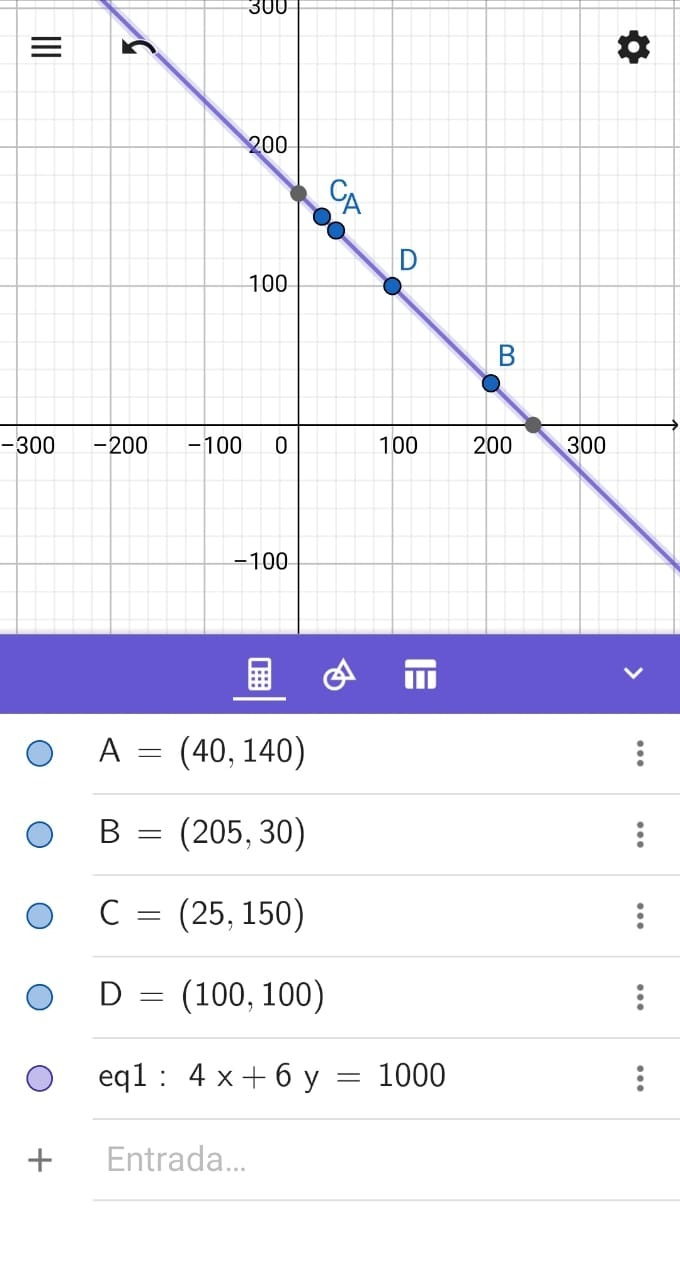
\includegraphics[width=120bp]{geogebra_eqlinear.png}
\end{figure}
\vspace{-2em}

As equações lineares já haviam aparecidos nas seções anteriores deste capítulo (localize-as!) e em todas elas, a representação geométrica das soluções também eram dadas por retas. Esse fato nos sugere a seguinte pergunta:	


\begin{observation}{}

\textbf{O conjunto solução de uma equação linear de duas incógnitas sempre pode ser representado geometricamente por uma reta no plano cartesiano?}


A fim de responder a esta pergunta, vamos fixar uma equação linear $ax + by = c$. Para facilitar a nossa análise, vamos organizar o raciocínio em dois casos:

\textbf{1\super{o} caso}: $b\neq 0$.  

Consideremos um par ordenado $(x_0,y_0)$ do plano cartesiano. Como $b \neq 0$, é permitido dividir por $b$. Assim, obtemos as equivalências a seguir:

$$
ax_0+by_0=c \ \Leftrightarrow \ by_0=c-ax_0 \ \Leftrightarrow \ y_0=\frac{c}{b}-\frac{a}{b}x_0.
$$

Assim, dizer que um ponto $(x_0,y_0)$ é uma solução da equação linear em questão é o mesmo que afirmar que ele é ponto do gráfico da função $f(x)=\frac{c}{b}-\frac{a}{b}x$. Com isso, concluímos que o conjunto solução da equação $ax+by=c$ coincide exatamente com o gráfico da função $f(x)=\frac{c}{b}-\frac{a}{b}x$.
	

%Se $a = 0$, $f$ é uma função constante e se $a\neq 0$, $f$ será uma função afim. 
Como vimos no Capítulo de Função Afim, independente do valor de $a$, o gráfico de $f$ é dado por uma reta (horizontal se $a =0$ e inclinada se $a\neq 0$), logo o conjunto solução da equação linear coincide com o gráfico da função $f$, sendo portanto representado geometricamente por uma reta no plano cartesiano.


\textbf{2\super{o} caso}: $b=0$.  

Como na equação linear $ax + by = c$ estamos supondo que os coeficientes $a$ e $b$ não são simultaneamente nulos, concluímos que $a\neq0$, uma vez que $b=0$. Dessa forma, a equação linear se reduz a $ax = c$. Assim, dizer que um ponto $(x_0,\frac{c}{b}-\frac{a}{b}x_0)$ é solução desta equação é o mesmo que escrever $ax_0=c$, ou equivalentemente, $x_0=\frac{c}{a}$. Como a incógnita $y$ não aparece nesta equação, não há qualquer restrição para o valor de $y_0$, isto é,$y_0$ pode ser qualquer número real. Concluímos então que o conjunto solução da equação linear será formado pelos pontos $(\frac{c}{a},y_0)$, onde $ y_0$ é qualquer. Se marcarmos todos esses pontos nos plano cartesiano, teremos exatamente a reta vertical que corta o eixo dos $x$ no número $\frac{c}{a}$.

Todo esse raciocínio nos mostrou que a resposta à pergunta é sim, ou seja:

\textbf{O conjunto solução de uma equação linear de duas incógnitas (em que os coeficientes $a$ e $b$ não são simultaneamente nulos) sempre pode ser representado geometricamente por uma reta no sempre pode ser representado geometricamente por uma reta no plano cartesiano.}

\end{observation}

Uma vez que respondemos à pergunta anterior, é natural que pensemos sobre outra questão:


\begin{observation}{}

\textbf{Toda reta no plano cartesiano representa o conjunto solução de uma equação linear de duas incógnitas?}

Vamos começar o raciocínio considerando uma reta qualquer do plano cartesiano. Novamente, vamos dividir o problema em dois casos:

\textbf{1\super{o} caso}: A reta não é paralela aos eixos coordenados.

Como visto no Capítulo de Função Afim, toda reta que não seja paralela aos eixos coordenados no plano cartesiano é o gráfico de uma função afim da forma $f(x) = ax+b$, $a\neq0$. Cada ponto $(x_0,y_0)$ pertencente a esta reta (ou seja, ao gráfico de $f$) satisfaz a igualdade $y_0=ax_0+b$, ou seja, $-ax_0+y_0=b$. Portanto, o conjunto de pontos da reta é precisamente o conjunto solução da equação linear $-ax+y=b$ nas incógnitas $x$ e $y$.

\textbf{2\super{o} caso}: A reta é paralela aos eixos coordenados.

Se a reta considerada for horizontal, ela intersecta o eixo $y$ em um número $y_0$. Assim, todos os pontos desta reta têm a segunda coordenada igual a $y_0$, ou seja, são da forma $(k, y_0)$, para qualquer $k$ real. Portanto, os pontos da reta compõem o conjunto solução da equação linear $0\cdot x+1\cdot y=y_0$.

Suponha agora que a reta seja vertical. Então ela intersecta o eixo $x$ em um número $x_0$. Todos os pontos desta reta têm a primeira coordenada igual a $x_0$, sendo da forma $(x_0,k)$ para qualquer $k$ real. Logo, os pontos da reta são o conjunto solução da equação linear $1\cdot x+0\cdot y=x_0$.

Portanto, a resposta para a segunda pergunta é: \textbf{Sim, toda reta do plano representa o conjunto solução de alguma equação linear de duas variáveis.}
\end{observation}

O nome “linear”{} usado para denominar essas equações que estamos estudando se justifica pelo fato demonstrado acima: os conjuntos soluções das equações da forma $ax+by=c$ correspondem exatamente às retas do plano cartesiano.

Como sabemos dois pontos distintos determinam uma reta, não é difícil esboçar a reta associada a uma equação linear $ax+by = c$. Se por exemplo, $b\neq 0$, basta atribuir dois valores distintos $a_1$ e $a_2$ para a incógnita $x$ e substituí-los na equação, isolando e calculando os valores correspondentes para $y$, digamos, $b_1$ e $b_2$. Assim, a reta procurada será aquela que passa por $(a_1,b_1)$ e $(a_2,b_2)$. Por exemplo, na equação $3x + y = 8$, substituindo $x=0$ na equação, obtemos $y = 8$ e substituindo $x = 1$, obtemos $y=5$, logo, a reta associada à equação é aquela que passa pelos pontos $(0,8)$ e $(1,5)$.  

No contexto mais geral, envolvendo um número maior de incógnitas, digamos $x_1,x_2, \ldots, x_n$, equações da forma $a_1x_1 + a_2x_2 + \ldots a_nx_n = c$, onde $a_1, a_2, \ldots, a_n, c$ são constantes, tais que $a_1, \ a_2, \ \ldots, \ a_n$ não são todos nulos,  também serão chamadas de lineares. 

\clearpage
\def\currentcolor{session1}
\begin{objectives}{Retas no Plano Cartesiano}
{
\begin{itemize}
\item Identificar equações de retas paralelas.
\end{itemize}
}{1}{1}
\end{objectives}
\begin{sugestions}{Retas no Plano Cartesiano}
{
\begin{itemize}
\item Professor, vale a pena estimular os alunos a construir as representações gráficas das três retas em um mesmo sistema de eixos, seja no papel, seja usando o GeoGebra.
\item Essa atividade pode ser feita tanto no Geogebra quanto no papel. Se fizer no Geogebra, basta entrar com as equações das retas para que se faça a representação gráfica dela. Se fizer no papel, lembre que da Geometria Euclidiana Plana,  para determinar uma reta no plano, basta conhecer dois de seus pontos.  
\item Na resolução do item \titem{b)} ajude seus alunos a encontrar soluções de uma das equações, levando-os a verificar que as mesmas também são solução para a outra.
\item Na resolução do item \titem{c}) sugira que os alunos manipulem algebricamente a equação $2$ de forma que se chegue na equação $1$.
\end{itemize}
}{1}{1}
\end{sugestions}
\begin{answer}{Retas no Plano Cartesiano}
{
\begin{enumerate}
\item As retas são iguais.
\item São as mesmas retas. Isso significa que o conjunto solução das equações são iguais.
\item A equação $2$ é a equação $1$ multiplicada por $-3.$
\item São paralelas. Não, pois tal ponto estaria na interseção das retas.
\item As equações diferem apenas no termo independente. Basta alterar a constante isolada, isto é, $2x+3y=k, k\in \mathbb{R}$.
\item Concorrente
\item O sistema possui solução única, que significa que as retas são concorrentes em um ponto
\end{enumerate}
}{1}
\end{answer}
\explore{Posições Relativas entre Retas no Plano}
\label{\detokenize{AF107-4:explorando-posiçoes-relativas}}\label{\detokenize{AF107-4::doc}}

\begin{task}{Retas no Plano Cartesiano}
\label{retas}
Na última seção, vimos que o conjunto solução de uma equação linear em duas incógnitas é representado por uma reta no plano. Considere as equações lineares a seguir:
\begin{align*}
\mbox{Equação} \ 1: 2x+3y=1;   &   \ \ \ \  \mbox{Equação} \ 2: -6x - 9y = -3;\\
\mbox{Equação}\ 3: 2x+3y=4;    & \ \ \ \ \mbox{Equação} \ 4: 3x + y = 5. \\
\end{align*}
\begin{enumerate}
\item{} 
Esboce a reta associada a Equação 1, em seguida, destaque 2 pontos dessa reta. Esses dois pontos são soluções da Equação? Justifique.

\item{}
Esboce a reta da Equação 2. Qual é a relação entre essa reta e a da Equação 1? Discuta com seus colegas o que isso significa com relação às soluções das Equações 1 e 2.

\item{}
Qual é a relação algébrica entre as Equações 1 e 2? Elabore exemplos de outras equações lineares que tenham a mesma relação.

\item{}
Esboce a reta da Equação 3. Qual é a relação entre as retas das Equações 1 e 3? Baseado nisso, diga se um ponto $(x_0,y_0)$ pode ser solução das Equações 1 e 3 simultaneamente? Justifique a sua resposta.

\item{}
Qual é a relação algébrica entre as Equações 1 e 3? Dê exemplos de outras equações que tenham a mesma relação.

\item{}
Trace a reta associada a Equação 4. Qual a relação dessa reta com as traçadas nos itens anteriores?

\item{}
Resolva o sistema formado pelas Equações 1 e 4 e relacione a solução com o que você observou no gráfico?

\end{enumerate}


\end{task}



\arrange{Posições Relativas entre Retas no Plano}
\label{\detokenize{AF107-4:posiçoes-relativas}}\label{\detokenize{AF107-4::doc}}

Nos itens \titem{a)}, \titem{b} e \titem{c} da atividade \hyperref[retas]{\textit{Retas no Plano Cartesiano}} vimos que algumas equações lineares, mesmo tendo coeficientes diferentes, representam a mesma reta no plano, ou seja, possuem o mesmo conjunto solução. Naquela atividade, a equação $-6x - 9y = -3$ é obtida multiplicando-se a equação $2x + 3y = 1$ por $-3$ e ambas essas equações possuíam mesmo conjunto solução, sendo representadas por uma mesma reta no plano cartesiano. Seria esse um fenômeno geral? Bem, vamos investigar!

\begin{example}{}
 Vamos começar com duas equações lineares múltiplas uma da outra por uma constante $k\neq0$ como segue:

\begin{center}
Equação 1: $ax+by=c$;  \ \ \ \ Equação 2: $kax+kby=kc$.
\end{center}

Se $(x_0,y_0)$ é uma solução da Equação 1, temos:

$$ax_0 +by_0=c.$$

Ao multiplicarmos ambos os lados dessa equação por $k$, temos:

$$kax_0 +kby_0=kc.$$

Ou seja, $(x_0,y_0)$ também é uma solução para Equação 2.

Por outro lado, se $(x_0,y_0)$ é uma solução para Equação 2, temos:

$$kax_0 +kby_0=kc.$$

Ao dividirmos ambos os lados dessa equação por $k$ (lembre-se que $k\neq 0$), temos:

$$ax_0 +by_0=c.$$

Assim, temos que $(x_0,y_0)$ também é uma solução para Equação 1. Duas equações que têm o mesmo conjunto solução são chamadas de \emph{equações equivalentes}. O raciocínio acima prova que \textbf{se duas equações que são múltiplas uma da outra são equivalentes e, portanto, são representadas por retas coincidentes no plano}. 
\end{example}

Com base nas ideias organizadas acima, as equações $3x - 6y = 4$ e $12x - 24y = 16$ representam retas coincidentes no plano, pois a segunda equação é obtida da primeira multiplicando-se a igualdade por 4.

Ainda na atividade \textit{\hyperref[retas]{Retas no Plano Cartesiano}} nos itens d e e, você estudou um caso de duas equações lineares que eram diferentes apenas pelo valor de seus coeficientes independentes. As retas correspondentes àquelas equações eram paralelas. Vamos deduzir aqui que este também é um fato geral. 


\begin{example}{}

Considere as Equações 3 e 4 abaixo:

\begin{center}
Equação 3: $ax+by=c_1$; \ \ \ \ Equação 4: $ax+by=c_2$;
\end{center}

onde $a$, $b$, $c_1$ e $c_2$ são constantes com $c_1 \neq c_2$. Vamos dividir nosso estudo em três casos:

\textbf{1\super{o} caso)} $b = 0$: As duas equações se reduzem a $ax = c_1$ e $ax = c_2$. Como $b$ é nulo e $a$ e $b$ não são nulos simultaneamente, temos $a\neq0$. Dividindo as equações por $a$, temos $x=\frac{c_1}{a}$ e $x=\frac{c_2}{a}$, que representam duas retas verticais e diferentes, uma vez que $c_1\neq c_2$. Assim, estas retas são paralelas.

\textbf{2\super{o} caso)} $a = 0$: Temos que b será não nulo. Repetindo o processo acima, veremos que as Equações 3 e 4 são equivalentes às equações $y=\frac{c_1}{b}$ e $y=\frac{c_2}{b}$, que correspondem a um par de retas horizontais e diferentes, logo, paralelas.

\textbf{3\super{o} caso)}: $a\neq0$ e $b\neq0$: Dividindo as Equações 3 e 4 por $b$ e isolando o termo que contém a incógnita $y$, vemos que estas equações são equivalentes respectivamente às equações $y=\frac{-a}{b}x+\frac{c_1}{a}$ e $y=\frac{-a}{b}x+\frac{c_2}{a}$. As retas correspondentes a essas equações são exatamente os gráficos das funções afins $f(x)=\frac{-a}{b}x+\frac{c_1}{a}$ e $g(x)=\frac{-a}{b}x+\frac{c_2}{a}$. As taxas de variação média de $f$ e $g$ são ambas iguais a $\frac{-a}{b}$, portanto, como vimos no capítulo de Função Afim, os gráficos dessas duas funções são dados por retas paralelas.

Deduzimos assim que \textbf{se duas equações lineares diferem apenas pelo seu coeficiente independente, elas definem retas paralelas}.
\end{example}

O raciocínio desenvolvido acima mostra que numa equação linear $ax+ by =c$, os coeficientes $a$ e $b$ das incógnitas x e y estão diretamente relacionados à inclinação da sua reta associada: quando $b = 0$, a reta é vertical; quando $a = 0$, é horizontal e quando $a\neq0$ e $b\neq0$, a inclinação da reta é igual à taxa de variação média da função afim $f(x)=\frac{-a}{b}x+\frac{c}{a}$, ou seja, $\frac{-a}{b}$.

Para ilustrar o raciocínio desenvolvido acima, considere as equações abaixo:

\begin{center}
(a) $3x + 5y = -3$; \ \ \       (b) $6x +10y = -6$; \ \   \       (c) $-12x -20y = -50$; \ \ \     (d) $4x + 2y = 1$.
\end{center}

A inclinação das retas dadas pelas equações lineares (a), (b) e (c) é a mesma, pois $\frac{-3}{5}=\frac{-6}{10}=\frac{-(-12)}{-20}$, logo, elas correspondem a retas paralelas (ou coincidentes) duas a duas no plano cartesiano. Em particular, como (b) é obtida multiplicando a equação (a) por $2$, estas equações são equivalentes e portanto determinam retas coincidentes no plano. Já a equação (d) tem inclinação igual a $\frac{-4}{2}=-2$, e portanto, diferente das demais. Logo, a reta que representa o conjunto solução da equação (d) terá um único ponto de interseção com cada uma das retas associadas às equações (a), (b) e (c). A figura a seguir ilustra esses fatos:

\begin{figure}[H]
\centering

\noindent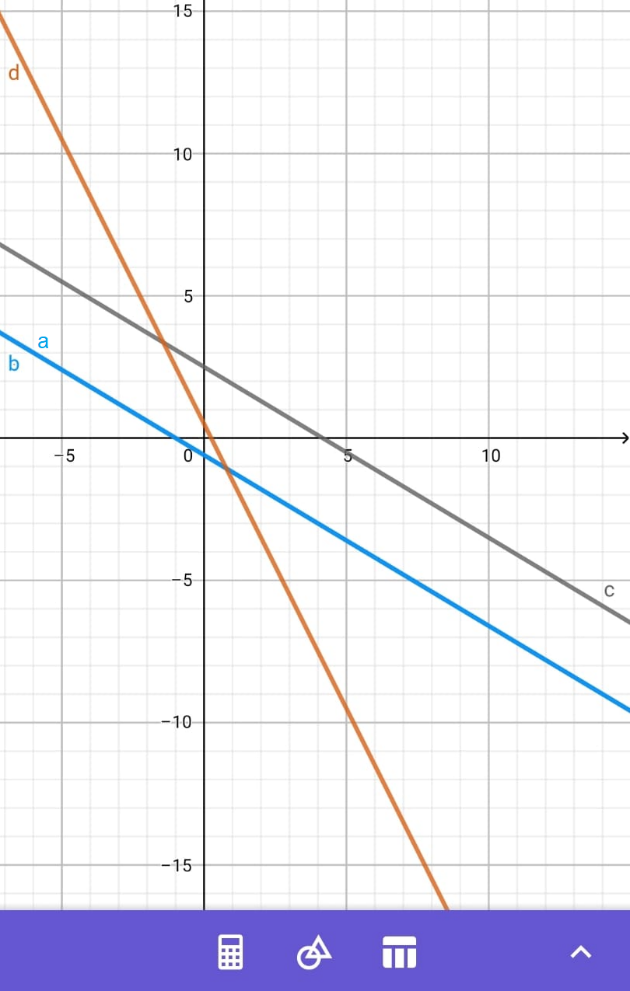
\includegraphics[width=125bp]{exemplo_relativas.png}
\end{figure}

\clearpage
\def\currentcolor{session2}
\begin{objectives}{Construindo Retas no Plano}
{
\begin{itemize}
\item Estudar equações equivalentes.
\item Consolidar o significado geométrico de equações equivalente. 
\end{itemize}
}{1}{2}
\end{objectives}
\begin{sugestions}{Construindo Retas no Plano}
{
\begin{itemize}
\item Nesse exercício, o objetivo é que o aluno perceba que é possível manipular a equação e escrever equações equivalentes a ela com os coeficientes que forem convenientes. Se possível, incentive seus alunos a plotar cada uma dessas equações com o GeoGebra, o que reforçará a ideia da equivalência entre elas, pois as suas representações ficarão sobrepostas quando construídas em um mesmo sistema de eixos
\end{itemize}
}{1}{2}
\end{sugestions}
\begin{answer}{Construindo Retas no Plano}
{
\begin{enumerate}
\item Multiplicando toda a equação por $-\dfrac{1}{3}$, encontramos $x-\dfrac{4}{3}y = -\dfrac{1}{3}$.
\item Multiplicando toda a equação por $\dfrac{1}{2}$, encontramos $\dfrac{3}{2x} + 2y =\dfrac{1}{2}$.
\item Multiplicando toda a equação por $\dfrac{1}{9}$, encontramos $\dfrac{1}{2}x + \dfrac{4}{9}y = \dfrac{1}{9}$.
\item Multiplicando toda a equação por $-\frac{7}{4}$, encontramos $-\dfrac{21}{4}x - 7y = - \dfrac{7}{4}$.
\item Multiplicando toda a equação por $5$, obtemos $15x + 20y = 5$.
\item Multiplicando toda a equação por $-\dfrac{2}{5}$, obtemos $-\dfrac{6}{5}x - \dfrac{8}{5}y = -\dfrac{2}{5}$.
\item $-12x+9y=-87$.
\item Para atender o que foi pedido no \titem{g}), pegue qualquer reta concorrente a $r$ que passe por $(8,1)$, divida a equação pelo coeficiente do $y$ e multiplique por $9$. Para atender as condições do item \titem{e)}, multiplique a equação encontrada em \titem{e)} por qualquer numero real não nulo. Para o item \titem{f)} é impossível achar outra opção, pois só existe uma única reta que cumpra as condições exigidas, assim, todas as equações são múltiplas umas das outras, portanto, apenas uma tem o coeficiente do $x$ igual a $6$.
\end{enumerate}
}{1}
\end{answer}

\practice{Posições Relativas entre Retas no Plano}
\label{\detokenize{AF107-4:praticando-posiçoes-relativas}}\label{\detokenize{AF107-4::doc}}

\begin{task}{Construindo Retas no Plano}

Considere a reta $r$ cuja equação é $3x + 4y = 1$. Em cada item abaixo, encontre uma equação linear em $x$ e $y$ tal que ela:


\begin{enumerate}
\item{}
Seja equivalente à equação do enunciado, com coeficiente de $x$ igual a $-1$;

\item{}
Seja equivalente à equação do enunciado, com coeficiente de $y$ igual a $2$;

\item{}
Seja equivalente à equação do enunciado, com coeficiente de $x$ igual a $\frac{1}{3}$;

\item{}
Seja equivalente à equação do enunciado, com termo independente igual a $5$;

\item{}
Represente uma reta paralela a $r$ e que passa pelo ponto $(2,5)$;

\item{}
Tenha o coeficiente do $x$ igual a $6$, represente uma reta paralela a $r$ e passe pelo ponto $(3,-7)$;

\item{}
Tenha coeficiente do $y$ igual a $9$, represente uma reta concorrente a $r$ e passe pelo ponto $(8,1)$.

\item{}	
Você consegue encontrar mais de uma equação linear que atenda o que foi pedido no item \titem{g)}? O mesmo é possível para os itens \titem{e)} e \titem{f)}? Por quê?

\item{}
Utilize o GeoGebra para plotar as retas correspondentes às equações obtidas por você nos itens \titem{e)}, \titem{f)} e \titem{g)} e confirmar se elas cumprem as propriedades pedidas nesses itens.
\end{enumerate}

\end{task}

\clearpage
\def\currentcolor{session1}
\begin{objectives}{Fazendo mais bolos}
{
\begin{itemize}
\item Resolver um sistema de equações lineares de duas incógnitas.
\item Abordagem geométrica ao problema de solução de sistema de equações lineares de duas incógnitas. 
\end{itemize}
}{1}{1}
\end{objectives}
\begin{sugestions}{Fazendo mais bolos}
{
Nessa atividade o aluno deverá encontrar a solução para um sistema de equações lineares de duas incógnitas. Como nenhum método de resolução foi apresentado ainda, recomenda-se que, ao se fazer os gráficos (no item c), os alunos testem valores que pareçam estar próximos ao ponto de interseção das retas.
}{1}{1}
\end{sugestions}
\begin{answer}{Fazendo mais bolos}
{
\begin{enumerate}
\item Sendo $x$ a quantidade de bolos de fubá e $y$ a de chocolate
\item $15x+18y =510$.
\item $4x+3y=100$
\item Incentive os alunos a que explorem tanto por construção usando lápis e papel quanto também que utilizem ambientes digitais, como o GeoGebra, por exemplo.
\item $10$ de fubá e $20$ de chocolate.
\end{enumerate}
}{1}
\end{answer}
\clearmargin
\begin{objectives}{Rede de Tráfego Rodoviário}
{
\begin{itemize}
\item Identificar um sistema linear com mais do que duas variáveis.
\item Resolver um sistema linear por escalonamento.
\end{itemize}
}{1}{2}
\end{objectives}
\begin{sugestions}{Rede de Tráfego Rodoviário}
{
O objetivo dessa atividade é dar um primeiro exemplo de sistema linear escalonado. Apesar dele possuir 6 incógnitas, o formato desse tipo de sistema permite que a cada incógnita que tem seu valor determinado permite que se calcule o valor de uma outra incógnita do sistema. Assim, a solução do sistema é facilmente determinada.
}{1}{2}
\end{sugestions}
\begin{answer}{Rede de Tráfego Rodoviário}
{
\begin{enumerate}
\item 
$\left \{
\begin{aligned}
x_1+x_2&=600\\
x_2+x_3&=650\\
-x_3+x_4&=-100\\
-x_4+x_5&=50\\
-x_5+x_6&=100
\end{aligned}
\right.$
\item $(x_1,x_2,x_3,x_4,x_5,x_6)=(300,300,350,250,300,400)$
\item Sim. No item $b)$, ao atribuir o valor $400$ à incógnita  foi possível encontrar um valor para as demais incógnitas de forma que esses valores compunham uma solução para o sistema do item \titem{a)}. Atribuindo outros valores a $x_6$ e repetindo o processo realizado no item \titem{b)} pode-se obter infinitas soluções para este mesmo sistema.
\end{enumerate}
}{1}
\end{answer}

\explore{Sistemas de Equações Lineares}
\label{\detokenize{AF107-5:explorando-sistemas-lineares}}\label{\detokenize{AF107-5::doc}}

\begin{task}{Fazendo mais bolos}
\label{mais_bolos}
Vamos voltar à fábrica de bolos da Tia Tatá? Sabemos que os bolos que mais vendem são os de fubá e o de chocolate e que custam $15$ reais e $18$ reais cada um, respectivamente.

\begin{figure}[H]
\centering

\noindent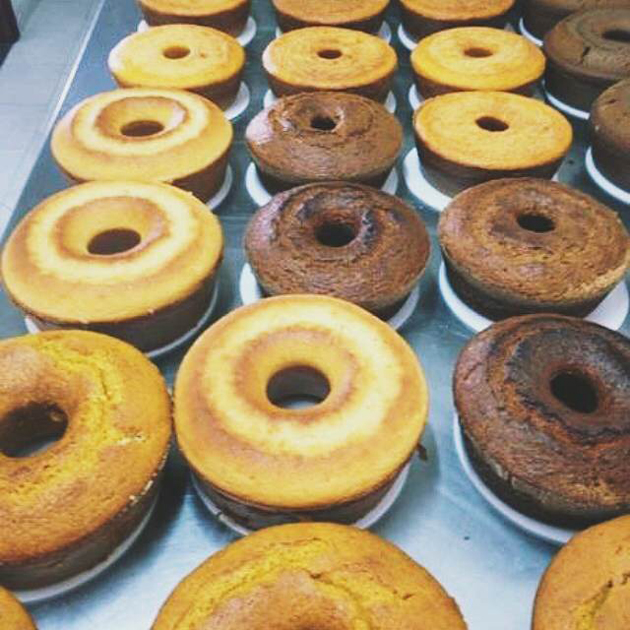
\includegraphics[width=300bp]{bolos.jpg}
\end{figure}

\begin{enumerate}
\item{}
Em determinado dia, a fábrica precisa faturar exatamente R\$ $510{,}00$ com a venda desses dois tipos de bolo. Escreva uma equação que relacione as possíveis quantidades de cada bolo que ela precisa vender;

\item{}
Na receita do bolo de chocolate usam-se $4$ ovos, enquanto na de fubá, usam-se $3$. Escreva uma equação que relacione a quantidade de bolos de chocolate e a quantidade de bolos de fubá e com um total de $100$ ovos;

\item{}
Num mesmo plano cartesiano, faça um esboço das representações gráficas dos conjuntos soluções das equações encontradas nos itens \titem{a)} e \titem{b)};

\item{}
Imagine que o dia em que é necessário se obter o faturamento de R\$ $510{,}00$ é o mesmo em que a fábrica dispõe dos 100 ovos. Assumindo que todos os bolos sejam vendidos, quantos bolos de cada sabor deverão ser produzidos?
\end{enumerate}



\end{task}



\begin{task}{Rede de Tráfego Rodoviário}
\label{trafego}

\begin{figure}[H]
\centering

\noindent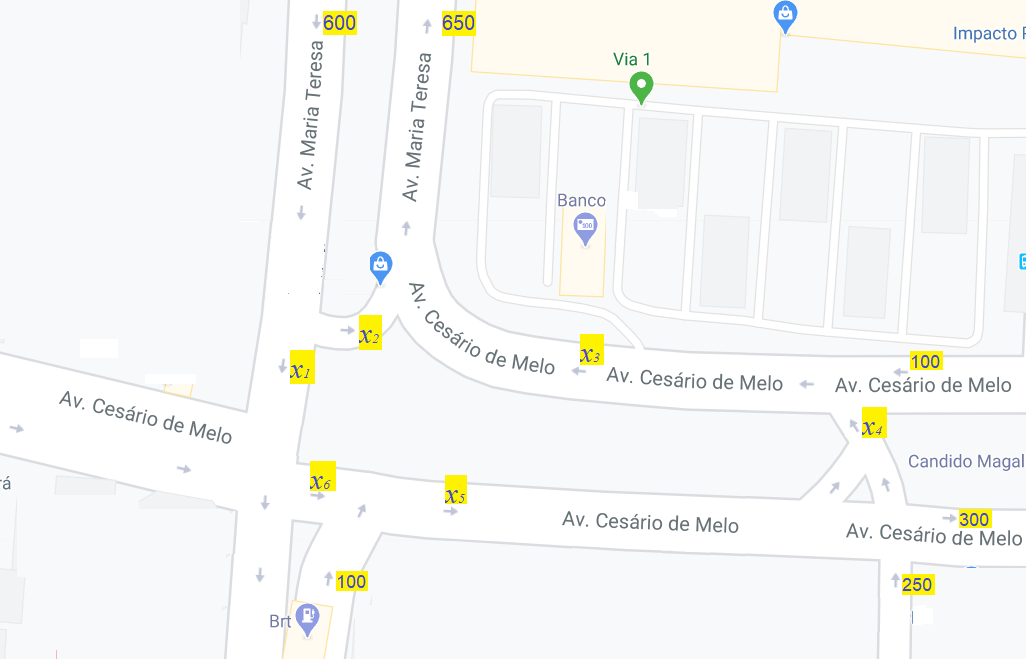
\includegraphics[width=400bp]{trafego.png}
\caption{Fonte: Adaptada do aplicativo Google Maps.}
\end{figure}

O mapa acima ilustra o trecho de uma rede rodoviária com grande movimento de carros em um bairro da cidade do Rio de Janeiro. Todas as avenidas destacadas no mapa são de mão única e as setas indicam o sentido em que os veículos trafegam sobre elas. Os valores destacados em amarelo em alguns trechos das avenidas representam o fluxo de veículos que passam por hora naquele trecho. Nessa rede de tráfego há conservação do fluxo de veículos, isto é, o fluxo de veículos que entra em uma bifurcação é igual ao fluxo de veículos que sai dessa bifurcação. Por exemplo, a figura mostra que por hora chegam $600$ veículos nesta rede através da Avenida Maria Teresa, sendo que na primeira bifurcação, uma certa quantidade $x_1$ de veículos continua em frente e outra quantidade $x_2$ entra pelo retorno da Avenida.  Pela conservação de fluxos temos:
$$
x_1 + x_2 = 600.
$$

\begin{enumerate}
\item{}
Com as informações que estão disponíveis no mapa e a conservação do fluxo de veículos, obtenha um sistema de equações envolvendo as incógnitas $x_1,x_2,..., x_6$.

\item{}
Suponha que um técnico da companhia de engenharia de tráfego aferiu que o valor da incógnita $x_6$ era de $400$ veículos por hora. Com essa informação e com o sistema obtido no item \titem{a)}, determine o valor das outras incógnitas destacadas no mapa. 

\item{}
O sistema que você obteve no item \titem{a)} tem mais de uma solução? Se sim, você consegue obter algumas?

\end{enumerate}

\end{task}




\arrange{Sistemas de Equações Lineares}
\label{\detokenize{AF107-5:sistemas-lineares}}\label{\detokenize{AF107-5::doc}}


Um sistema de equações é dito \emph{linear} quando ele é formado apenas por equações lineares. Você provavelmente já estudou a resolução de sistemas lineares com duas equações e duas incógnitas há alguns anos, pelos métodos de \emph{substituição} e de \emph{adição}. Vamos relembrá-los?

O \emph{método de substituição} consiste em isolar uma das incógnitas em uma das equações e substituir essa incógnita na outra equação pela expressão equivalente a ela determinada previamente. Vamos ver um exemplo:
\begin{equation*}
\left\{
\begin{aligned}
2x+3y&=7\\
x-4y&=\frac{5}{3}
\end{aligned}
\right.
\end{equation*}
Isolando $x$ na segunda equação, obtemos $x = 4y + \frac{5}{3}$. Substituindo o valor de $x$ na primeira equação:

$$
2x+3y = 7 \ \Rightarrow \ 2(4y + \frac{5}{3}) + 3y = 7 \ \Rightarrow \ 8y + \frac{10}{3} + 3y = 7 \ \Rightarrow \ 11y = \frac{11}{3} \ \therefore \ y = \frac{1}{3}.
$$

Substituindo o valor obtido para $y$ na segunda equação, obtemos: 

$$
x = 4y + \frac{5}{3} \ \Rightarrow \ x = 4 \cdot \frac{1}{3} + \frac{5}{3} \ \Rightarrow \ x = \frac{9}{3} \ \therefore \ x = 3.
$$
Portanto, o sistema possui uma única solução, dada pelo par $(3, \frac{1}{3})$.

Poderíamos resolver esse mesmo sistema de equações de outra maneira, usando o \emph{método da adição}. Nesse método, trabalhamos com equações equivalentes determinadas de forma que seja possível, somando membro a membro as equações do sistema, cancelar os termos de uma das incógnitas. De fato, vamos multiplicar a segunda equação do sistema por $-2$, obtendo uma equação equivalente. 
\begin{equation*}
\left\{
\begin{aligned}
2x+3y&=7\\
x-4y&=\frac{5}{3} &\textcolor{red}{\cdot(-2)}
\end{aligned}
\right.
\implies
\left\{
\begin{aligned}
2x+3y&=7\\
-2x+8y&=\frac{-10}{3}
\end{aligned}
\right.
\end{equation*}
Repare que ao somarmos as equações membro a membro, a incógnita $x$ desaparecerá da expressão da soma:

$$
(2x + 3y) + (-2x + 8y) = 7 + -\frac{10}{3} \ \Rightarrow \ 11y = \frac{11}{3} \ \therefore \ y = \frac{1}{3}.
$$

Agora, basta substituir o valor obtido para $y$ em alguma das duas equações do sistema, e como já vimos acima, vemos que teremos $x = 3$.


\paragraph{Quantas soluções um sistema linear com 2 incógnitas pode ter?}

Nas seções anteriores vimos que o número de soluções em um sistema de equações pode ser bem diverso. Na seção \emph{Organizando - Sistemas de Equações}, vimos exemplos de sistemas que possuem, uma, duas ou até mesmo nenhuma solução. Veremos agora que quando o sistema de equações em duas incógnitas é \textbf{linear}, o formato do conjunto solução será bem particular. 
Lembra-se da interpretação geométrica dada ao conjunto solução das equações lineares em duas incógnitas $x$ e $y$? Essas soluções correspondem a uma reta no plano cartesiano. Se temos um sistema linear nestas mesmas incógnitas, as suas soluções são dadas por \textbf{pontos que pertencem simultaneamente a cada uma das retas} correspondentes às equações lineares desse sistema. Sabemos que toda reta tem infinitos pontos. Sabemos também que duas retas do plano ou não se intersectam (são paralelas), ou se intersectam num único ponto (são concorrentes) ou são iguais (são coincidentes). Portanto, as possibilidades para o conjunto solução de um sistema linear em duas incógnitas é:

\begin{enumerate}
\item{}
\textbf{Possui uma única solução}. Este é o caso em que as retas associadas às equações lineares concorrem em um único ponto, que será exatamente a solução do sistema;

\item{}
\textbf{Possui infinitas soluções}. Este é o caso em que todas as retas associadas às equações lineares são iguais, isto é, são todas coincidentes entre si.

\item{}
\textbf{Não existe solução}. Este é o caso em que não existe um ponto que pertença a todas as retas simultaneamente.


\end{enumerate}

A figura abaixo ilustra, geometricamente, as três possibilidades de conjunto solução apresentadas acima, para o caso de um sistema linear com duas incógnitas e três equações. Repare que no caso de infinitas soluções, as três retas associadas às equações são coincidentes.
\begin{figure}[H]
\centering
\noindent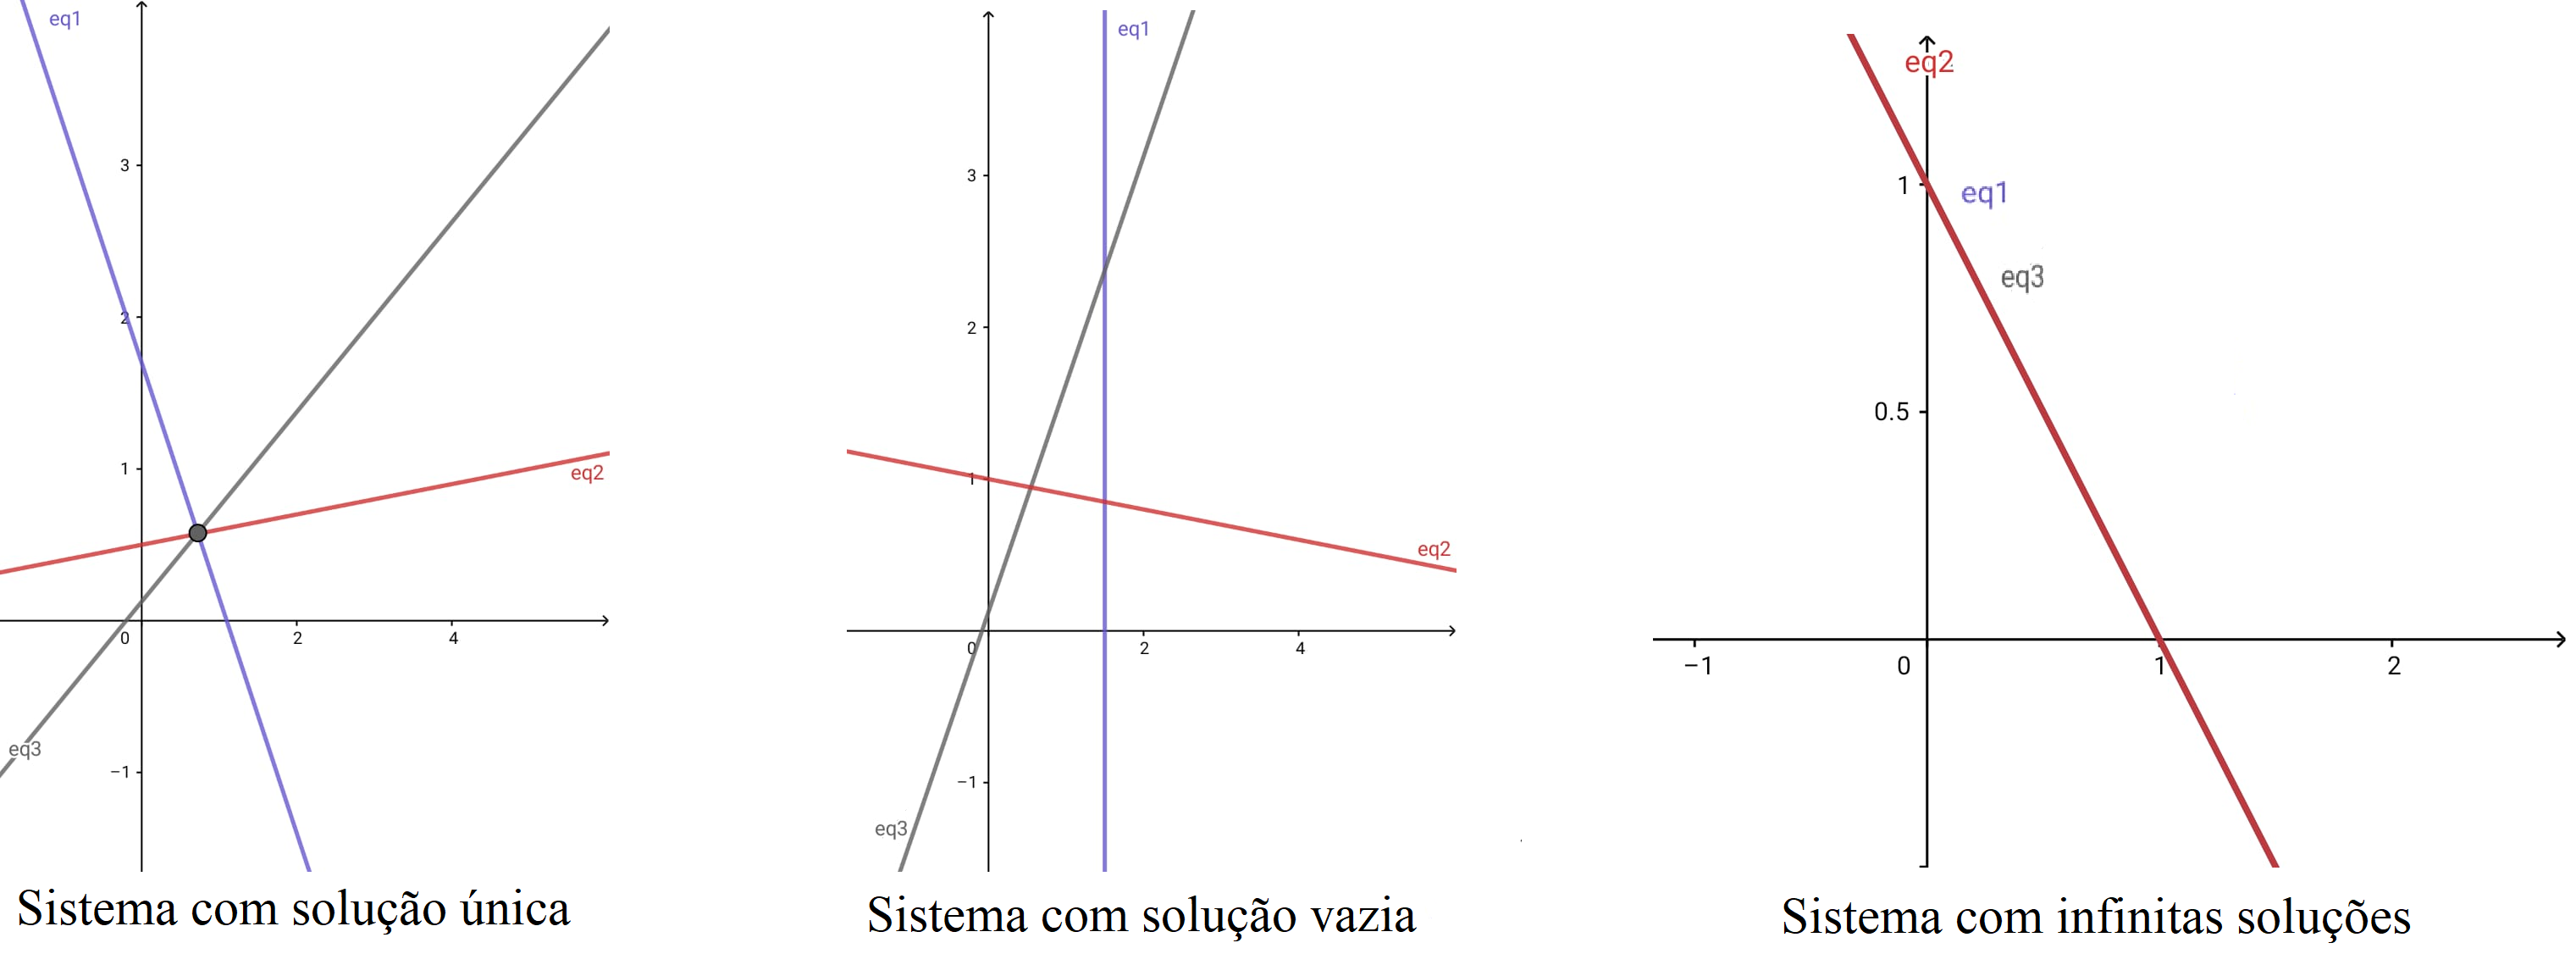
\includegraphics[width=400bp]{solucoes_sistema.png}
\end{figure}


Você observou que quando resolvemos um sistema linear pelo método da adição, realizamos uma manipulação algébrica em uma das equações de modo que pudéssemos cancelar uma incógnita do sistema? Essa é uma estratégia bastante interessante e que pode ser ampliada para a resolução de sistemas maiores. Vamos conhecer melhor essa estratégia de resolução? Para isso, antes precisamos conhecer um tipo de sistema que será bem interessante para nós: os sistemas escalonados.

\paragraph{Sistemas escalonados}

No item \titem{a)} da atividade \hyperref[trafego]{\textit{Rede de Tráfego Rodoviário}}, você viu que o seguinte sistema linear modelava matematicamente as informações sobre o fluxo de veículos em um complexo de avenidas:
\begin{equation*}
\left\{
\begin{aligned}
x_1+x_2&=600\\
x_2+x_3&=650\\
x_3-x_4&=100\\
x_4-x_5&=-50\\
x_5-x_6&=100
\end{aligned}
\right.
\end{equation*}
Apesar de possuir seis incógnitas, descobrir soluções desse sistema não é tão complicado. Por exemplo, ao atribuir o valor $400$ à incógnita $x_6$, através da quinta equação, se obtém que $x_5=500$. “Subindo”{} para a quarta equação, substituindo esse valor encontrado para $x_5$ se determina que $x_4=450$. Continuando desse modo, “subindo”{} gradativamente nas equações, se determinam valores para todas as incógnitas de forma que, para eles, todas as igualdades do sistema são satisfeitas, isto é, obtemos uma solução desse sistema. Se iniciássemos atribuindo um outro valor para $x_6$, digamos $300$, poderíamos repetir o mesmo processo, obtendo outra solução para o sistema: calculamos $x_5$ na quinta equação, obtendo $400$, e depois “subimos”{} nas equações e substituindo os valores obtidos, encontrando $x_4=350$, $x_3=450$, $x_2=200$ e $x_1=400$. Note que esse sistema tem, portanto, mais de uma solução.

	Observe que esse sistema pôde ser organizado em um formato bem específico: a incógnita $x_1$ não aparece efetivamente a partir da segunda equação, ou seja, os coeficientes de $x_1$ nessas outras equações são todos nulos; a incógnita $x_2$ não aparece a partir da terceira equação, a incógnita $x_3$ não aparece a partir da quarta equação e assim sucessivamente até chegar à última equação. Note que é correto afirmar que a incógnita $x_5$ não aparece a partir da sexta equação, pois... não há uma sexta equação. Um sistema linear com este formato é chamado de \textbf{escalonado}.
	
	De maneira mais precisa, dizemos que um sistema linear está \textbf{escalonado} se é possível enumerar suas incógnitas $x_1,x_2,...x_n$ e ordenar as suas equações lineares de forma que $x_1$ não aparece efetivamente a partir da segunda equação, $x_2$ não aparece a partir da terceira equação e assim sucessivamente até chegarmos à última incógnita $x_n$ ou até a última equação do sistema.
	
	A seguir temos mais um exemplo de sistema escalonado. Quando organizamos as equações escrevendo cada incógnita de forma alinhada verticalmente como ilustrado abaixo ($x_4$ embaixo de $x_4$, $x_3$ embaixo de $x_3$, ...), visualmente se forma nos espaços “em branco”{} uma espécie de “escada”:

\begin{figure}[H]
\centering

\noindent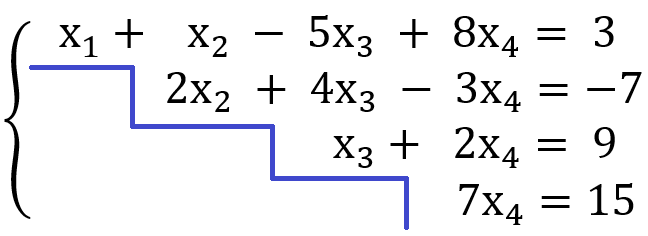
\includegraphics[width=200bp]{escalonado.png}
\end{figure}

Vamos analisar os sistemas a seguir:

\begin{enumerate}[label=\titem{(\Roman*)}]

\begin{minipage}{.45\linewidth}
\centering
\item 
$
\left\{
\begin{aligned}
x+y-z&=1\\
2y-z&=8\\
z&=1
\end{aligned}
\right.
$
\end{minipage}
\begin{minipage}{.45\linewidth}
\centering
\item 
$
\left \{
\begin{aligned}
2x+4&y-3z+w&=1\\
7&y+3z&=1\\
x+2&y-z&=0
\end{aligned}
\right.
$
\end{minipage}
\end{enumerate}






O sistema \titem{(I)} está escalonado. Aparentemente o sistema \titem{(II)} não está escalonado, porém, ele está sim: ao invés de listar as incógnitas na ordem $x, \ y, \ z$ e $w$, organizamos na ordem $w, x, y, z$. Também alternamos a posição da segunda equação com a terceira. Note que esse tipo de mudança não altera as soluções do sistema pois as equações, na prática, continuam as mesmas.

\begin{equation*}
\left \{
\begin{aligned}
w+2x+4y-3z&=1\\
x+2z-z&=0\\
7y+z&=0
\end{aligned}
\right.
\end{equation*}

\paragraph{Escalonando e Resolvendo Sistemas Lineares}

Veremos agora que todo sistema linear pode ser transformado em um sistema escalonado que mantém exatamente as mesmas soluções do primeiro. Este processo será chamado de \emph{escalonamento} de um sistema linear. O fato do sistema estar escalonado facilita o cálculo das suas soluções.

Essencialmente, o processo de escalonamento utiliza as mesmas técnicas que já vinhamos utilizando até aqui. São elas:

\begin{enumerate}
\item{} 
Trocar duas ou mais equações de posição;
\item{}
Multiplicar uma equação (todos os seus termos) por uma constante não nula;
\item{} Trocar uma equação pela soma, membro a membro, dela com outra equação do sistema.
\end{enumerate}


Observe que ao aplicar a técnica \titem{a)} evidentemente não se alteram as soluções do sistema pois as suas equações continuam as mesmas. Por sua vez, as técnicas \titem{b)} e \titem{c)} são as mesmas usadas no método da adição para sistemas lineares com 2 equações e 2 incógnitas. Pode-se provar que estas técnicas também não alteram as soluções do sistema.

Repare que, combinando as técnicas \titem{b)} e \titem{c)}, obtemos a técnica:

\begin{enumerate}\setcounter{enumi}{3}
\item Trocar uma equação pela soma, membro a membro, dela com uma outra equação do sistema que foi multiplicada por uma constante não nula.
\end{enumerate}


Vamos ver alguns exemplos de como utilizá-las para se escalonar e resolver um sistema?



\begin{example}{}
Iremos escalonar e resolver o seguinte sistema:

\begin{equation*}
\left \{
\begin{aligned}
x+2y+z&=12\\
x-3y+5z&=1\\
2x-y+3z&=10
\end{aligned}
\right.
\end{equation*}

Procuramos sempre deixar a primeira incógnita da primeira equação com coeficiente 1. É o caso deste exemplo, mas se não fosse, utilizaríamos as técnicas \titem{a)} ou \titem{b)} para deixar o sistema com esse formato.

Iremos eliminar primeiro a incógnita $x$ na segunda e na terceira equações. Usamos a técnica \titem{d)} trocando a segunda equação pela soma dela pela primeira multiplicada por $-1$:
\begin{equation*}
\left \{
\begin{aligned}
x+2y+z&=12 &&\textcolor{red}{\cdot(-1)} &&\vspace{1ex}\textcolor{blue}{\downarrow}\\
x-3y+5z&=1 &&\quad\textcolor{red}{+}  &&\textcolor{blue}{\leftarrow}\\
2x-y+3z&-10
\end{aligned}
\right.
\implies
\left \{
\begin{aligned}
x+2y+z&=12\\
-5y+4z&=-11\\
2x-y+3z&=10
\end{aligned}
\right.
\end{equation*}

Agora, usamos a técnica \titem{d)} novamente, trocando a terceira equação pela soma dela pela primeira multiplicada por $-2$:
\begin{equation*}
\left \{
\begin{aligned}
x+2y+z&=12 &&\textcolor{red}{\cdot(-2)} &&\vspace{1ex}\textcolor{blue}{\downarrow}\\
-5y+4z&=-11 &&&&\vspace{1ex}\textcolor{blue}{\downarrow}\\
2x-y+3z&=10 &&\quad\textcolor{red}{+}  &&\textcolor{blue}{\leftarrow}
\end{aligned}
\right.
\implies
\left \{
\begin{aligned}
x+2y+z&=12\\
-5y+4z&=-11\\
-5y+z&=-14
\end{aligned}
\right.
\end{equation*}

Para concluir o escalonamento, basta eliminar a incógnita $y$ da terceira equação. Usamos a técnica \titem{d)} novamente, trocando a terceira equação pela sua soma com a segunda equação multiplicada por $-1$:
\begin{equation*}
\left \{
\begin{aligned}
x+2y+z&=12 \\
-5y+4z&=-11  &&\textcolor{red}{\cdot(-1)} &&\vspace{1ex}\textcolor{blue}{\downarrow}\\
2x-y+3z&=10 &&\quad\textcolor{red}{+}  &&\textcolor{blue}{\leftarrow}
\end{aligned}
\right.
\implies
\left \{
\begin{aligned}
x+2y+z&=12\\
-5y+4z&=-11\\
-3z&=-3
\end{aligned}
\right.
\end{equation*}

Obtivemos portanto um sistema escalonado. Na terceira equação obtemos:
$$
-3z=-3 \ \ \therefore z = 1. 
$$ 
Substituindo o valor encontrado para $z$ na segunda equação:
$$
-5y +4z = -11 \ \implies -5y + 4 = -11 \ \implies -5y = -15 \ \therefore \ y = 3.
$$
Por fim, substituindo os valores encontrados para $y$ e $z$ na primeira equação, obtemos:
$$
x + 2y + z = 12 \ \implies \ x + 6 + 1 = 12 \ \therefore x = 5.
$$
Concluímos que o sistema possui uma única solução: $x = 5, \ y = 3, \ z = 1$, ou de forma mais resumida, podemos representar esta solução lista ordenada $(5,3,1)$.

Quando um sistema linear \emph{possui uma única solução}, dizemos que ele é um \textbf{sistema possível e determinado} (S.P.D.).
\end{example}



\begin{example}{}
Escalone e resolva o sistema:

\begin{equation*}
\left \{
\begin{aligned}
3x+y+z&=5\\
x-2y+3z&=-4\\
-2x+4y-6&=8
\end{aligned}
\right.
\end{equation*}

Começamos usando a técnica \titem{a)} alternando a posição da primeira equação com a segunda. Dessa forma, o coeficiente de $x$ na primeira equação passa a ser $1$: 
\begin{equation*}
\left \{
\begin{aligned}
x-2y+3z&=-4\\
3x+4y+z&=-6\\
-2x+4y-6z&=8
\end{aligned}
\right.
\end{equation*}

Em seguida, usamos a técnica \titem{d)} na segunda equação, trocando-a pela soma dela com a primeira equação multiplicada por $-3$:

\begin{equation*}
\left \{
\begin{aligned}
x-2y+3z&=-4 &&\textcolor{red}{\cdot(-3)} &&\vspace{1ex}\textcolor{blue}{\downarrow}\\
3x-4y+z&=-6 &&&&\vspace{1ex}\textcolor{blue}{\downarrow}\\
-2x+4y-6z&=8 &&\quad\textcolor{red}{+}  &&\textcolor{blue}{\leftarrow}
\end{aligned}
\right.
\implies
\left \{
\begin{aligned}
x-2y+3z&=-4\\
2y-8z&=6\\
-2y+4y-6z&=8
\end{aligned}
\right.
\end{equation*}

Repetimos o processo agora trocando a terceira equação pela soma dela com a primeira multiplicada por $2$. Notemos que ao fazer essa operação, todos os coeficientes da última equação vão se anular:

\begin{equation*}
\left \{
\begin{aligned}
x-2y+3z&=-4 &&\textcolor{red}{\cdot(+2)} &&\vspace{1ex}\textcolor{blue}{\downarrow}\\
2y-8z&=6 &&&&\vspace{1ex}\textcolor{blue}{\downarrow}\\
-2x+4y-6z&=8 &&\quad\textcolor{red}{+}  &&\textcolor{blue}{\leftarrow}
\end{aligned}
\right.
\implies
\left \{
\begin{aligned}
x-2y+3z&=-4\\
2y-8z&=6\\
0x+0y+0z&=0
\end{aligned}
\right.
\end{equation*}
Assim, concluímos o escalonamento. Observe que quaisquer valores que se deem às incógnitas $x$, $y$ e $z$ sempre fornecerão uma solução para a terceira equação (compare com a resposta obtida no item \titem{e)} da Atividade \hyperref[batalha-naval]{\textit{Batalha Naval}}), de modo que ela é \emph{irrevelevante} para o cálculo das soluções do sistema. Podemos descartá-la, ficando apenas com as duas primeiras equações:
\begin{equation*}
\left \{
\begin{aligned}
x-2y+3z&=-4\\
2y-8z&=6
\end{aligned}
\right.
\end{equation*}

Este último sistema também está escalonado. Isolando $y$ na segunda equação, obtemos:
$$
2y - 8z = 6 \ \implies \ 2y = 6 + 8z \ \therefore y = 3 + 4z.
$$
Substituindo este valor encontrado para $y$ na primeira equação:
$$
x - 2y +3z = -4 \ \implies \ x -2(3+4z) + 3z = -4 \ \implies \ x -6 - 8z +3z = -4 \ \therefore \ x = 2 +5z.
$$
Notemos que, se fizermos $z = 0$, pelos cálculos acima, obteremos que $x = 2$ e $y = 3$, e portanto, esses três valores compõem uma solução do sistema. Se porém fizermos $z = 3$, obteremos $x = 17$ e $y = 15$, logo, esses três valores fornecem outra solução para o sistema. Poderíamos proceder assim para qualquer outro valor real escolhido para$z$. Dessa forma, vemos que todas as soluções desse sistema são da forma:
$$
x = 2 + 5k, \ \ \ y = 3 + 4k \ \ \ \mbox{e} \ \ \ z = k, 
$$   
para qualquer $k \in \mathbb{R}$. Portanto, esse sistema linear tem \emph{infinitas soluções}. Quando isso ocorre, dizemos que o \textbf{sistema é possível e indeterminado} (S.P.I.).
\end{example}

\clearpage
\def\currentcolor{session2}
\begin{objectives}{Classificando Sistemas Lineares}
{
\begin{itemize}
\item Resolver um sistema linear por escalonamento.
\item Classificar um sistema linear em relação à cardinalidade de seu conjunto solução.
\end{itemize}
}{1}{1}
\end{objectives}
\marginpar{\vspace{-2em}}
\begin{sugestions}{Classificando Sistemas Lineares}
{
Exercício para resolução de sistemas já escalonados e sua classificação como sistema possível determinado (SPD), sistema possível indeterminado (SPI) ou sistema impossível (SI).
}{1}{1}
\end{sugestions}
\begin{answer}{Classificando Sistemas Lineares}
{
\begin{enumerate}
\item $(x,y,z)=(\dfrac{29}{2},-10,-3)$ , SPD.
\item $(x,y,z)=(-7;\dfrac{z+5}{2},z);z\in \mathbb{R}$, SPI.
\item $(x,y,z,w)=(\dfrac{97-11w}{15},\dfrac{-3w-9}{5}, \dfrac{-w-1}{3},w); w\in \mathbb{R}$, SPI.
\item $(x,y,z,w)=(\dfrac{75}{8},\dfrac{21}{8},\dfrac{-1}{2},\dfrac{3}{8})$, SPD.  
\end{enumerate}
}{1}
\end{answer}
\begin{objectives}{Dieta Nutricional}
{
\begin{itemize}
\item Aplicar sistemas lineares em contexto nutricional.
 \item Resolver um sistema linear por escalonamento. 
\end{itemize}
}{1}{1}
\end{objectives}
\marginpar{\vspace{-2em}}
\begin{sugestions}{Dieta Nutricional}
{
Neste exercício primeiro o aluno precisa escrever as equações que modelam o fenômeno (isso o aluno já está acostumado, pois já fez algumas modelagens nas atividades \textit{\hyperref[teatro]{Faturamento de um teatro}, \hyperref[clube]{Clube de Esportes}, \hyperref[mais_bolos]{Fazendo mais bolos}} e \textit{\hyperref[trafego]{Rede de Tráfego}} ) e, em seguida, deve escalonar o sistema obtido, seguindo os passos apresentados anteriormente.
}{1}{1}
\end{sugestions}
\clearmargin
\marginpar{\vspace{.5em}}
\begin{answer}{Dieta Nutricional}
{
\begin{enumerate}
\item 
$
\left \{
\begin{aligned}
10x_1+10x_2+20x_3&=100\\
50x_1+40x_2+10x_3&=300\\
30x_1+10x_2+40x_3&=200
\end{aligned}
\right.  
$
\item $\displaystyle(x_1,x_2,x_3)=(\frac{25}{8},\frac{25}{8},\frac{15}{8})$.
\item $\displaystyle\frac{1625}{4}$ gramas.
\end{enumerate}
}{1}
\end{answer}
\begin{objectives}{Trajetória de uma bola de futebol}
{
\begin{itemize}
\item Aplicar um sistema linear em contexto de modelagem de trajetória.
\end{itemize}
}{1}{2}
\end{objectives}
\begin{sugestions}{Trajetória de uma bola de futebol}
{
Professor, o item \titem{c)} dessa atividade é uma excelente oportunidade para que se trabalhe com os alunos a determinação das coordenadas do vértice de uma parábola não pelas fórmulas clássicas ($(x_v,y_v)=(\frac{-b}{2a}, \frac{-\Delta}{4a})$), mas observando a simetria da parábola em relação a uma reta perpendicular ao eixo $0x$ passando pelo vértice, portanto, pode-se obter $x_v$ como sendo o ponto médio entre as raízes e o $y_v=f(x_v)$. 
}{1}{2}
\end{sugestions}
\clearmargin
\begin{answer}{Trajetória de uma bola de futebol}
{
\begin{enumerate}
\item 
$
\left \{
\begin{aligned}
25a-5b+c&=0\\
6{,}25a-2{,}5b+c&=5\\
6{,}25a+2{,}5b+c&=0
\end{aligned}
\right.
$
\item $(a,b,c)=(-\dfrac{2}{5},-1,5)$.
\item $5{,}625$m.
\end{enumerate}
}{1}
\end{answer}


\begin{example}{}
Vamos alterar levemente o sistema do Exemplo 2, mudando apenas o coeficiente independente da última equação:


\begin{equation*}
\left \{
\begin{aligned}
3x+y+z&=5\\
x-2y+3z&=-4\\
-2x+4y-6z&=9
\end{aligned}
\right.
\end{equation*}

Ao fazermos o processo de escalonamento, obteremos o seguinte sistema:

\begin{equation*}
\left \{
\begin{aligned}
x-2y+3z&=-4\\
2y-8z&=6\\
0x+0y+0z&=1
\end{aligned}
\right.
\end{equation*}
Observe que a terceira equação linear não possui solução, pois para quaisquer valores escolhidos para $x, y$ e $z$, o primeiro membro nunca será igual a $1$. Portanto, o sistema linear deste exemplo \emph{não possui solução}. Quando isto ocorre, dizemos que o \textbf{sistema é impossível} (S.I.).
\end{example}



\practice{Sistemas de Equações Lineares}
\label{\detokenize{AF107-5:praticando-sistemas-lineares}}\label{\detokenize{AF107-5::doc}}

\begin{task}{Classificando Sistemas Lineares}

Os sistemas lineares abaixo estão escalonados. Classifique-os em relação ao número de soluções (S.P.D., S.P.I. ou S.I.).

\begin{minipage}{\linewidth}
\begin{enumerate}[leftmargin=0pt]
\begin{multicols}{2}
\centering
\item

$
\left \{
\begin{aligned}
2x+3y-2z&=5\\
y-4z&=2\\
-3z&=9
\end{aligned}
\right.
$

\columnbreak

\item
$
\left \{
\begin{aligned}
-x-2y+z&=2\\
2y-z&=5
\end{aligned}
\right.
$

\end{multicols}
\begin{multicols}{2}
\centering

\item
$
\left \{
\begin{aligned}
x+z-z+w&=5\\
5y-3z+2w&=-8\\
-3z-w&=-3
\end{aligned}
\right.
$


\columnbreak

\item
$
\left \{
\begin{aligned}
x+y+3z-4w&=9\\
y-4z+w&=5\\
-z+4w&=2\\
2w&=-1
\end{aligned}
\right.
$
\end{multicols}
\end{enumerate}
\end{minipage}
\end{task}

\vspace{-1em}
\begin{task}{Dieta Nutricional}
Um nutricionista está elaborando uma dieta para um paciente que está com deficiência de vitamina C, cálcio e magnésio. Uma das refeições da dieta será composta por três alimentos com quantidades medidas em porções de $50$ g, de forma que os totais em miligramas (mg) dos nutrientes necessários sejam atingidos. A tabela abaixo contém as informações nutricionais dos três alimentos desta refeição:

\begin{table}[H]
\centering
\begin{tabu} to \textwidth{|c|c|c|c|e{3,5cm}|}
\hline
\tmcol{5}{|c|}{Miligramas de nutrientes por porção de 50g de alimento} \\
\hline
\tcolor{Nutriente} & \tcolor{Alimento 1 (mg)} & \tcolor{Alimento 2 (mg)} & \tcolor{Alimento 3 (mg)} & \tcolor{Total de  nutrientes  necessários (mg)} \\
\hline
Vitamina C & 10 & 10 & 20 & 100  \\
\hline
Cálcio & 50 & 40 & 10 & 300 \\
\hline
Magnésio & 30 & 10 & 40 & 200 \\
\hline
\end{tabu}
\end{table}

\begin{enumerate}
\item{}
Denote por $x_1$, $x_2$ e $x_3$ a quantidade de porções dos alimentos 1, 2 e 3 respectivamente que compõem uma refeição contendo exatamente a quantidade necessária de Vitamina C, Cálcio e Magnésio a serem ingeridas pelo paciente. Utilizando a tabela acima, escreva um sistema linear nas incógnitas $x_1$, $x_2$ e $x_3$ que represente essa situação;

\item{}

Escalone e resolva o sistema obtido no item \titem{a)}, classificando-o.

\item{}
Qual será o peso total de comida ingerida nesta refeição, considerando que ela contém apenas os alimentos 1, 2 e 3? 

\end{enumerate}
\end{task}


\begin{task}{Trajetória de uma bola de futebol}
\label{trajetoria}
\begin{figure}[H]
\centering
\noindent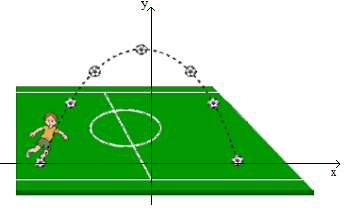
\includegraphics[width=300bp]{fadonelinho}
\caption{Adaptado de: \href{https://profes.com.br/felipes.rocha/blog/lancamento-obliquo-e-o-futebol}{Profes}}
\end{figure}

Após ver o vídeo em que Nelinho chuta a bola para fora do estádio, Mateus ficou fã do jogador e está praticando chutes altos com sua bola de futebol no campinho que há nas proximidades de sua casa. Mateus dá um chute na bola, que segue a trajetória de uma parábola. Considere que, numa visão frontal, considerou-se um sistema de coordenadas cartesianas como o da figura, onde o eixo $x$ é paralelo à linha lateral do campo e o eixo $y$ é perpendicular ao plano do campo. Ao longo da trajetória, a bola parte do ponto $(-5,0)$, passa pelo ponto $(-2.5, 5)$ e toca o solo no ponto $(2.5, 0)$. Considere a função quadrática $f(x) = ax²+bx+c$ que modela a trajetória da bola.

\begin{enumerate}
\item{}
Utilizando as informações sobre os pontos do sistema de coordenadas informados no enunciado pelos quais a bola passa no decorrer do movimento, obtenha um sistema de 3 equações nas 3 incógnitas $a$, $b$ e $c$.

\item{}
Escalone e resolva o sistema do item \titem{a)};

\item{}
Determine a altura máxima atingida pela bola após o chute dado por Mateus.

\end{enumerate}




\end{task}


\know{Interpolação Polinomial}

 Na Atividade \textit{\hyperref[trajetoria]{Trajetória de uma bola de futebol}}, você verificou que existe uma única função quadrática cujo gráfico passa por três pontos dados no plano cartesiano. O processo de encontrar uma função cujo gráfico passa por uma quantidade finita de pontos dados é denominado \textbf{interpolação de pontos}. A interpolação de pontos costuma ser aplicada quando se estuda um problema envolvendo duas grandezas representadas pelas variáveis $x$ e $y$ respectivamente, tais que $y$ é uma função de $x$, digamos $y = h(x)$. Esta função $h$ pode ter uma expressão analítica muito complicada e na maioria das vezes, desconhecida, e o máximo que se conhece sobre ela é uma lista finita $A_1 = (x_1, y_1)$, $A_2 = (x_2, y_2)$,..., $A_n = (x_n, y_n)$ de pontos de seu gráfico. Através da interpolação dos pontos $A_1$, ..., $A_n$, procura-se obter uma função $f$ cujo gráfico passe por esses pontos, que seja definida por uma expressão mais simples e que tenha o gráfico parecido com o da função $h$.  
 
As \textbf{funções polinomiais} são aquelas definidas através de expressões da forma $f(x) = a_0 + a_1x + a_2x^2 + \ldots +a_nx^n$, onde $a_0, \ a_1, \ldots , \ a_n$ são constantes reais. Se $a_n$ é não nulo, a maior potência de $x$ que aparece na expressão $f(x)$ é $x^n$. Neste caso, dizemos que $f$ é uma função polinomial de \textbf{grau $n$}. As funções afins e quadráticas, estudadas nos capítulos anteriores, são exemplos de funções polinomiais de graus 1 e 2 respectivamente. Repare que o cálculo das imagens das funções polinomiais envolvem apenas as operações elementares de adição, subtração e multiplicação de números reais, o que favorece o cálculo dessas imagens do ponto de vista computacional. 

Chamamos de \textbf{interpolação polinomial} o procedimento de encontrar uma função polinomial que interpola um conjunto finito de pontos dados. A figura abaixo ilustra um exemplo de interpolação polinomial de uma função $h$ (gráfico azul) os 5 pontos $A$,$B$,$C$,$D$ e $E$ do seu gráfico, aproximando-a por uma função polinomial $f$ (gráfico vermelho). Note que o comportamento do gráfico de $f$ é muito parecido com o de h nas proximidades desses 5 pontos.

\begin{figure}[H]
\centering
\noindent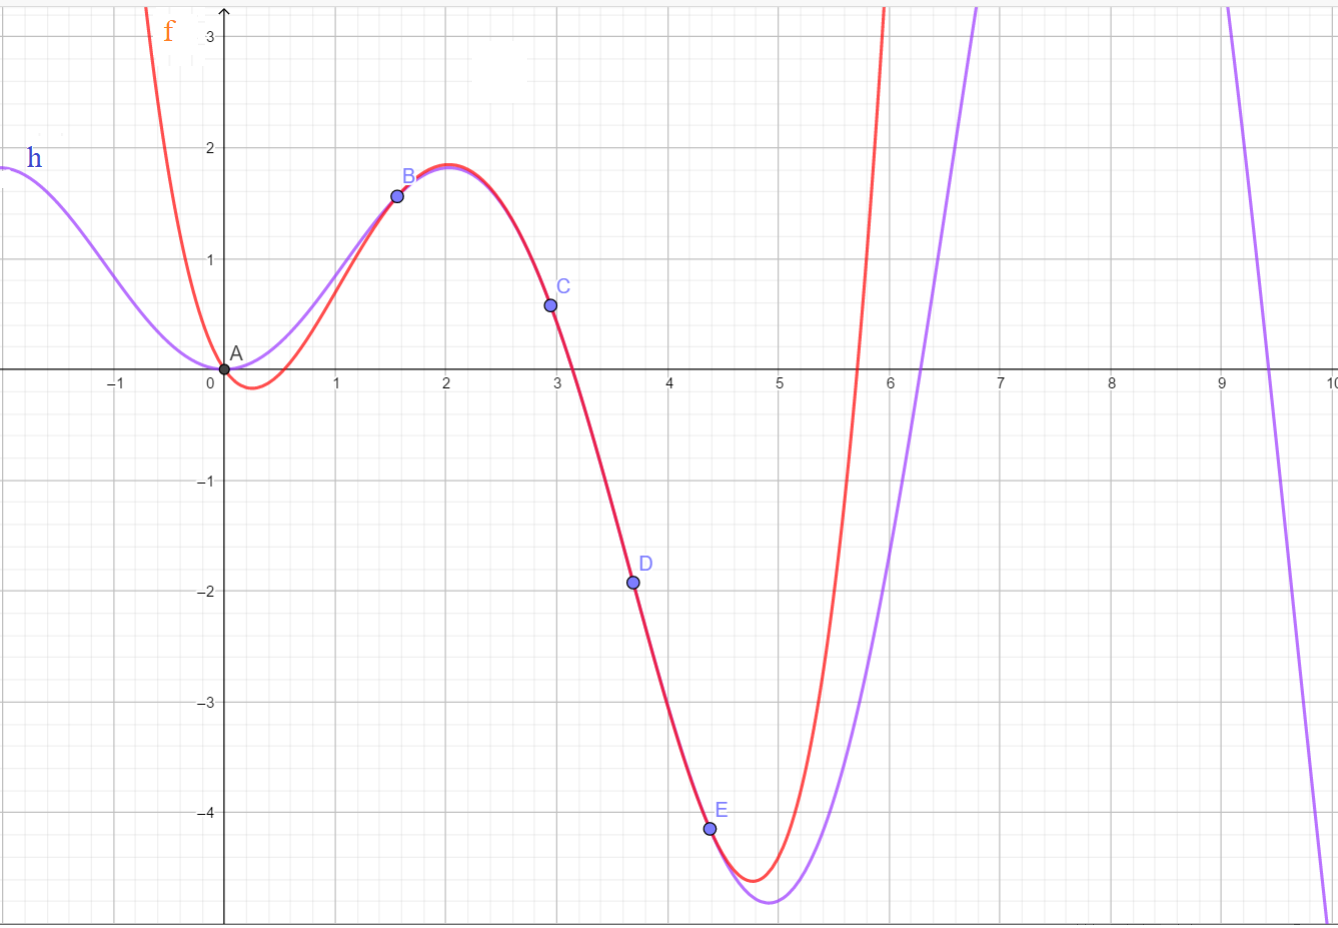
\includegraphics[width=325bp]{interpolacao}
\end{figure}

A Teoria dos Sistemas Lineares que estamos estudando permite demonstrar que dada uma lista $A_0 = (x_0, y_0), \ A_1 = (x_1, y_1), \ldots ,\ A_n = (x_n, y_n)$ de $n+1$ pontos conhecidos do plano cartesiano, se as abscissas $x_0, \ x_1, \ldots , \ x_n$ forem distintas duas a duas, então existe uma única função polinomial de grau $n$ cujo gráfico passa por esses pontos. De fato, se $f$ é uma função polinomial de grau $n$, temos que:
$$
f(x) = a_0 + a_1x + ... + a_nx^n,
$$

onde $a_n \neq 0$. Se o gráfico de $f$ passa por $A_0 = (x_0,y_0)$, então $f(x_0) = y_0$. Substituindo essa última informação na expressão de f temos:
$$
a_0 + x_0\cdot a_1 + ... + {x_0}^n \cdot a_n = y_0,
$$
o que nos dá uma equação linear nas incógnitas $a_0, \ a_1, \ ..., \ a_n$, cujos coeficientes dessas incógnitas são respectivamente $1, x_0, \ldots, {x_0}^n$ e o coeficiente independente é $y_0$. Repetindo o mesmo cálculo para os demais pontos da lista, obtém-se um sistema linear de $n+1$ equações nas $n+1$ incógnitas $a_0, \ a_1, \ldots, \ a_n$:

\begin{equation*}
\left \{
\begin{aligned}
a_0+x_0\cdot a_1+&\cdots+x_0^n\cdot a_n=y_0\\
a_0+x_1\cdot a_1+&\cdots+x_1^n\cdot a_n=y_0\\
&\quad\vdots\\
a_0+x_n\cdot a_1+&\cdots+x_n^n\cdot a_n=y_0\\
\end{aligned}
\right.
\end{equation*}

o qual pode-se provar que é possível e determinado! Assim, existem únicos valores para as incógnitas $a_0, ..., a_n$ que fornecem uma solução para o sistema, logo existe uma única função polinomial que interpola os pontos $A_0, ..., A_n$. Repare que, na atividade \textit{\hyperref[trajetoria]{Trajetória de uma bola de futebol}}, foram dados os três pontos do plano: $A_0 = (-5,0)$, $A_1 = (-2.5, 5)$ e $A_2 = (2.5, 0)$ o que permitiu a você determinar uma (única!) função polinomial de grau $2$ (função quadrática) que interpola esses pontos. 


\begin{knowledge}

Nos últimos quarenta anos, a \textbf{Tomografia Computadorizada} se consolidou como um dos métodos mais importantes de diagnóstico na medicina do corpo humano. Ela possibilita a aquisição de imagens paralelas e espacialmente consecutivas e cortes axiais com melhor contraste entre os tecidos do que a radiografia convencional, possibilitando a análise de regiões que com outras técnicas, não poderiam ser observadas satisfatoriamente.

Assim, a Tomografia Computadorizada é um meio não invasivo
de obter imagens do interior de um corpo. Essas imagens são obtidas a partir do exterior do objeto pela medição das intensidades dos feixes de Raios-X que atravessam esse corpo. Esses dados são processados
por um computador e a seção transversal computada é exibida num monitor de vídeo.
\begin{figure}[H]
\centering
\noindent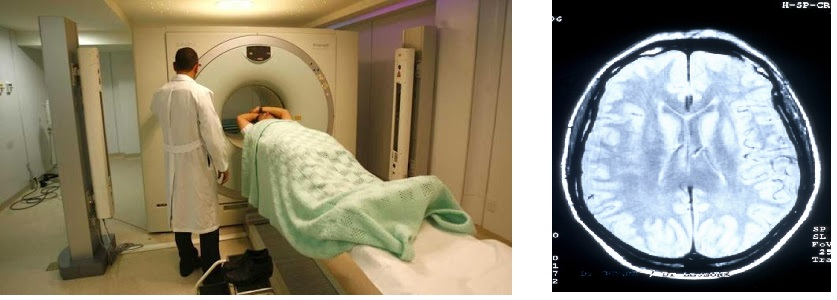
\includegraphics[width=300bp]{tomografia}
\end{figure}
A construção de uma imagem da Tomografia requer encontrar \textbf{soluções aproximadas de sistemas de equações lineares com muitas equações e muitas incógnitas}. Para compreender melhor o processo de construção da imagem, imaginemos que a seção transversal física do paciente seja a própria imagem dividida em \emph{pixels}. Os \emph{pixels} são pequenos quadrados monocromáticos que formam a imagem, ou seja, são os “elementos básicos”{} da imagem. Como o paciente é bombardeado inúmeras vezes por feixes de Raios-X, cada \emph{pixel} será “igualmente bombardeado”{} por estes feixes, em diversas direções, à medida que o tomógrafo gira. Para construir a imagem da Tomografia é necessário determinar a densidade de Raios-X retida em cada \emph{pixel}. A densidade de Raios-X em cada pixel é interpretada pelo computador através de uma tonalidade de cinza. Como o tecido humano absorve ou desvia densidades diferentes de Raios-X, a imagem distingue os diversos tecidos e órgãos.

\begin{figure}[H]
\centering
\noindent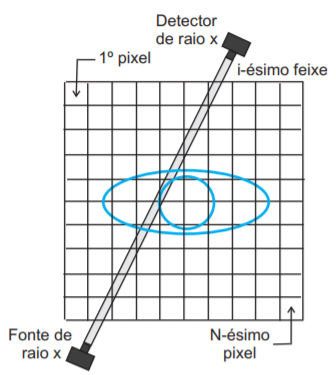
\includegraphics[width=175bp]{pixel}
\caption{Fonte: Livro do Howard Anton.}
\end{figure}

Para compreender melhor a ideia dos cálculos que permitem obter as imagens do exame, considere uma simplificação do campo de visão em apenas $9$ \emph{pixels}, que foram "escaneados"{} com $12$ feixes de Raios-X, cujas densidades são indicadas na figura a seguir:

\begin{figure}[H]
\centering
\noindent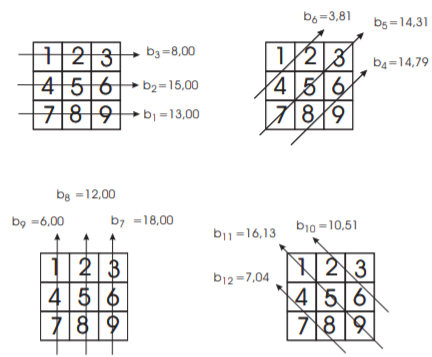
\includegraphics[width=300bp]{pixel2}
\caption{Fonte: Livro do Howard Anton.}
\end{figure}

Denotamos por $x_1$ a densidade de Raios-X absorvidas no pixel $1$, $x_2$ a densidade de Raios-X absorvidas no pixel $2$ e assim sucessivamente. Por outro lado, respresentamos por $b_1$ a densidade do 1\super{o} feixe de Raios-X, por $b_2$ a densidade do 2\super{o} feixe de Raios-X e assim sucessivamente. Para cada feixe de \emph{pixels}, sabe-se que \textbf{a sua densidade feixe é igual à soma das densidades de Raios-X absorvidas em todos os \emph{pixels} pelos quais ele atravessa}. Analisando a imagem acima, temos que o 1\super{o} feixe atravessa os \emph{pixels} $7$, $8$ e $9$, logo, a densidade $b_1$ desse feixe é igual a soma das densidades absorvidas por esses pixels. Isto é:
$$
x_7 + x_8 + x_9 = b_1 = 13,00,
$$
que é uma equação linear nas incógnitas $x_7$, $x_8$ e $x_9$. Fazendo mesmo raciocínio para os outros $11$ feixes com densidades $b_2, b_3, \ldots, b_{12}$, obtemos outras equações lineares, que juntas compõem o seguinte sistema linear:

\begin{figure}[H]
\centering
\noindent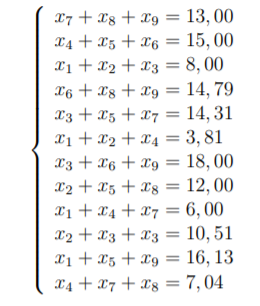
\includegraphics[width=140bp]{sistemao}
\end{figure}

As soluções desse sistema nos permitem determinar as densidades de Raios-X absorvidas em cada \emph{pixel} e assim, o computador colore esse pixel com uma tonalidade de cinza associada a essa densidade, formando no seu conjunto, a imagem da Tomografia. 

Repare que o que fizemos aqui foi uma simplificação do processo de geração da imagem, visto que há máquinas de Tomografia que trabalham com mais de $260.000$ \emph{pixels}, o que acaba gerando sistemas lineares com um número enorme de equações e incógnitas. Tais sistemas são resolvidos computacionalmente através de algoritmos muito eficientes no tempo de cálculo de suas soluções.
\end{knowledge}




\know{Sistemas Lineares com 3 Incógnitas}

Neste capítulo, você aprendeu que as equações lineares em $2$ incógnitas correspondem exatamente à retas no plano cartesiano. Além disso, você também viu que a solução de um sistema linear em $2$ incógnitas é geometricamente interpretado pelo conjunto de pontos do plano que pertencem simultaneamente a todas as retas associadas às equações desse sistema. 

Um sistema linear em $2$ incógnitas é S.P.D. exatamente quando todas as retas dadas pelas equações do sistema são concorrentes em um ponto $P$ do plano. Ele será S.P.I. quando todas as equações do sistemas forem representadas pela mesma reta do plano. Por fim, ele será S.I. quando não houver um ponto do plano que pertença a todas as retas simultaneamente.

Assim como os pontos de um plano estão em correspondência biunívoca com o conjunto de todos os pares ordenados $(x,y)$ de números reais, pode-se provar que \textbf{existe uma correspondência biunívoca entre os pontos do espaço com as listas ordenadas} $(x,y,z)$ de $3$ números reais. Soluções gerais de equações em três incógnitas $x$, $y$ e $z$ podem ser interpretadas geometricamente como objetos do espaço. Em particular, pode-se demonstrar que a solução geral de uma equação linear da forma:
$$
ax + by +cz = d,
$$ 
corresponde a um \textbf{plano} no espaço! 

Dessa forma, o \emph{conjunto solução de um sistema linear com $3$ equações e $3$ incógnitas pode ser visto como o conjunto de pontos que pertencem ao mesmo tempo aos $3$ planos correspondentes às suas equações}. Vamos interpretar geometricamente as possibilidades para o conjunto solução desse tipo de sistema em termos das posições relativas entre esses planos no espaço:

\begin{enumerate}
\item{}
\textbf{Sistema Possível e Determinado} (S.P.D.): Neste caso, haverá apenas uma única solução. Isso só é possível quando os três planos associados às equações do sistema forem  transversais dois a dois, ambos tendo um ponto comum, como na figura a seguir:

\begin{figure}[H]
\centering
\noindent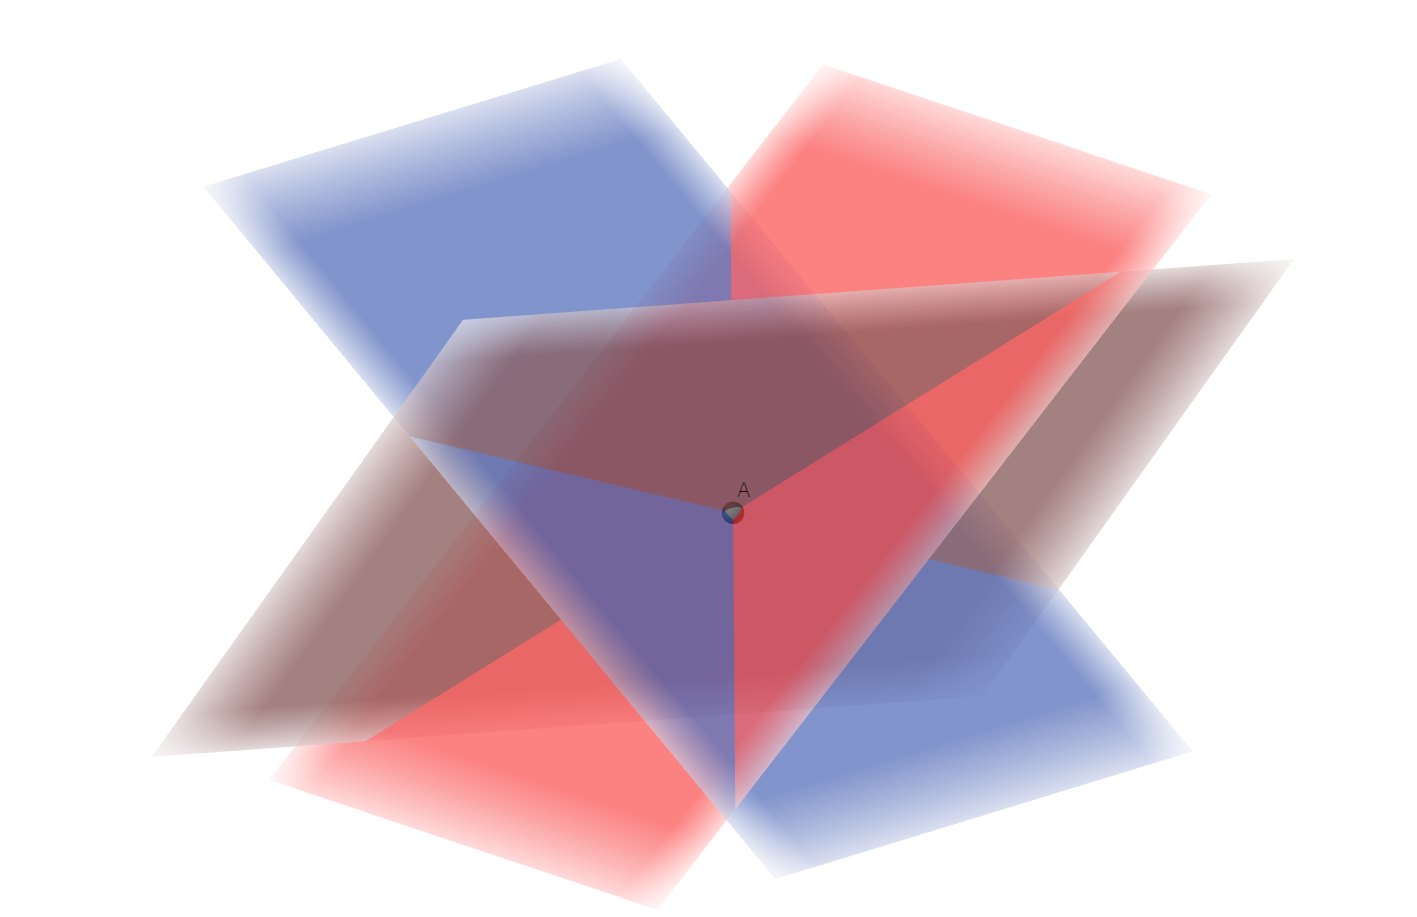
\includegraphics[width=200bp]{planos}
\caption{Três planos com um único ponto em comum.}
\end{figure}

\item{} 
\textbf{Sistema Possível e Indeterminado} (S.P.I.): Neste caso, haverá infinitos pontos que pertencem ao mesmo tempo aos três planos. Isso ocorre em exatamente duas situações: (i) quando os três planos são coincidentes (figura \ref{coin123}); (ii) dois planos são coincidentes e o terceiro é transversal a eles (figura \ref{2coin1t}). Nesse caso, a interseção entre os três planos é uma reta, que contém infinitos pontos; (iii) os três planos são distintos dois a dois, e ambos possuem a mesma reta em comum (figura \ref{3disti}).

\begin{figure}[!htb]
\begin{minipage}[b]{0.30\linewidth}

\includegraphics[width=\textwidth]{spi1}
\caption{Três planos coincidentes.}\label{coin123}
\end{minipage} \hfill
\begin{minipage}[b]{0.30\linewidth}
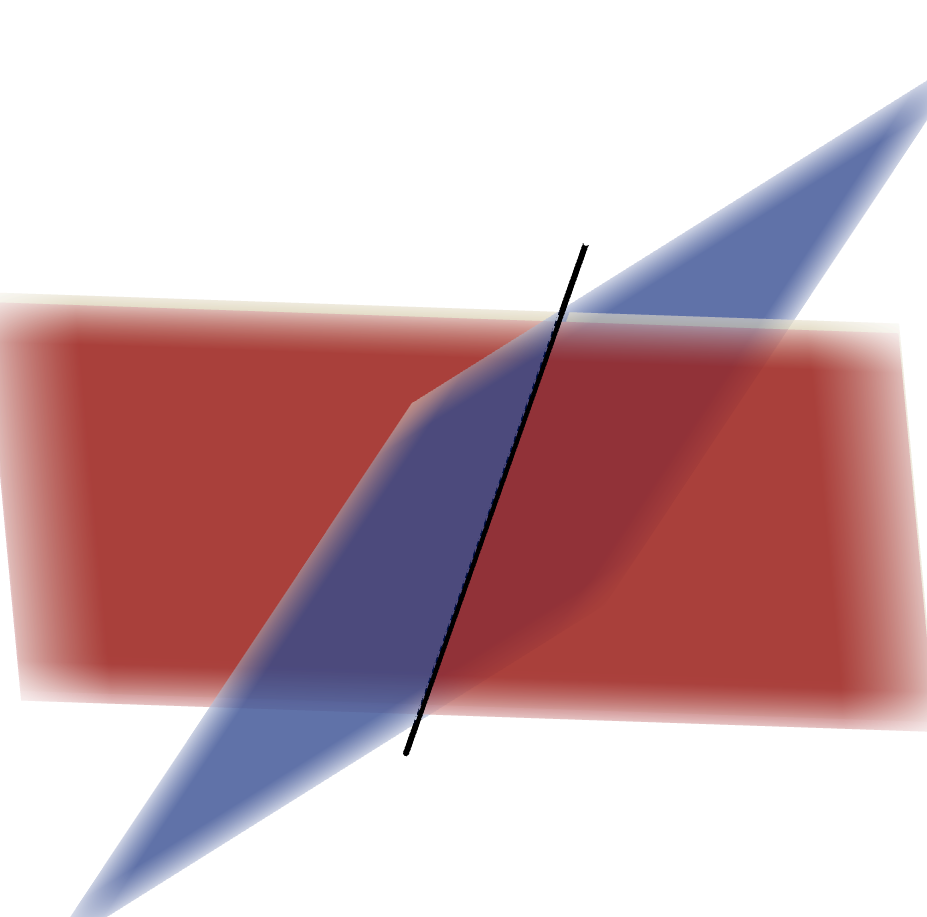
\includegraphics[width=\textwidth]{spi2}
\caption{Dois planos coincidentes e um transversal com uma reta em comum.}\label{2coin1t}
\end{minipage} \hfill
\begin{minipage}[b]{0.30\linewidth}

\includegraphics[width=\textwidth]{spi3}
\caption{Três planos distintos dois a dois com uma reta em comum.}\label{3disti}
\end{minipage}
\end{figure}

\item{} 
\textbf{Sistema Impossível} (S.I.): Neste caso, não haverá pontos que pertençam simultaneamente aos três planos. Há um total de 4 configurações possíveis para os planos: (i) dois planos são coincidentes e o terceiro é diferente e paralelo a eles; (ii) dois planos são diferentes e paralelos e o terceiro é transversal a eles; (iii) os três planos são distintos e paralelos dois a dois; (iv) os três planos são transversais dois a dois e não possuem ponto em comum. 

\begin{figure}[H]
\begin{minipage}{0.45\linewidth}
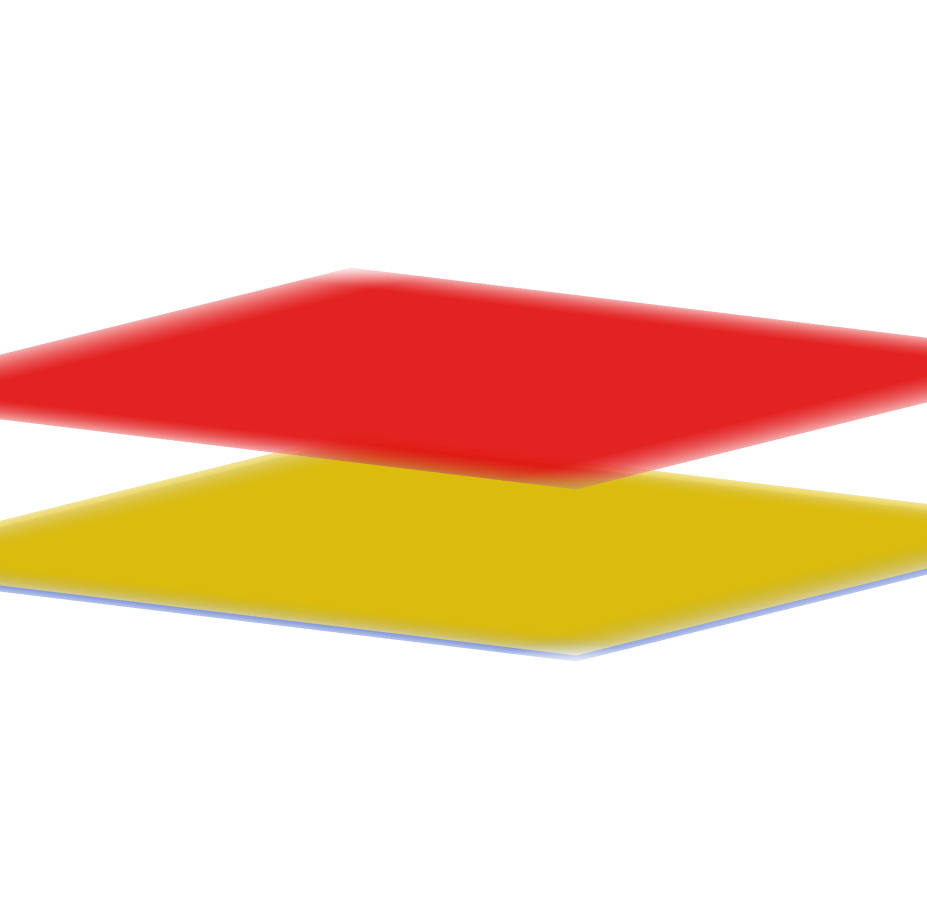
\includegraphics[width=150bp]{si1}
\caption{Dois planos coincidentes e um difetente e paralelo aos outros.}
\end{minipage} \hfill
\begin{minipage}{0.45\linewidth}

\includegraphics[width=150bp]{si3}
\caption{Planos distintos e paralelos entre si.}
\end{minipage} 
\end{figure}

\begin{figure}[H]
\begin{minipage}{0.45\linewidth}

\includegraphics[width=150bp]{si2}
\caption{Dois planos coincidentes e um difetente e paralelo aos outros.}
\end{minipage} \hfill
\begin{minipage}{0.45\linewidth}

\includegraphics[width=150bp]{si4}
\caption{Planos distintos e paralelos entre si.}
\end{minipage} 
\end{figure}

\end{enumerate}


 

\cleardoublepage
\def\currentcolor{session1}
\begin{objectives}{Locadora de carros}
{
\begin{itemize}
\item Reconhecer o significado geométrico das desigualdades.
 \item Estabelecer conexão entre o conceito de desigualdade e sua simbologia matemática.
\end{itemize}
}{1}{1}
\end{objectives}
\begin{sugestions}{Locadora de carros}
{
\begin{itemize}
\item Nessa atividade, pretende-se levar o aluno a perceber a relação entre a expressão “menor que” e o símbolo matemático $<$, bem como identificar uma representação gráfica da solução de uma inequação.
\item Incentive seus alunos a escrever as respostas tanto em termos literais (usando palavras) quanto em termos matemáticos (usando a notação matemática).
\end{itemize}
}{1}{1}
\end{sugestions}
\begin{answer}{Locadora de carros}
{
\begin{enumerate}
\item Até $40$ km.
\item Distâncias entre $20$ km e $120$ km.
\item A locadora $P$.
\item  $20$ km e $100$ km. 
\item Locadora $P$: entre $20$ km e $100$ km.
Locadora Q: de $1$ km a $20$ km ou distâncias superiores a $100$ km.
\end{enumerate}
}{1}
\end{answer}
\explore{Inequações em uma Incógnita}
\label{\detokenize{AF107-6:inequacoes}}\label{\detokenize{AF107-6::doc}}

Nesta seção, estudaremos as \emph{inequações} que é um conceito matemático utilizado para repreesentar algebricamente um problema que envolve uma desigualdade. Você muito provavelmente já estudou alguns tipos de inequação no Ensino Fundamental. Assim como no caso de sistemas lineares, as noções de funções afim e quadrática permitirá que aprimoremos o nosso conhecimento sobre inequações e de como resolvê-las. 


\begin{task}{Locadora de carros (Adaptada do ENEM 2015)}
\label{locadora}
Atualmente existem diversas locadoras de veículos, permitindo uma concorrência saudável para o mercado, fazendo com que os preços se tornem acessíveis. Nas locadoras \emph{Possante} ($P$) e \emph{Qualicarro} ($Q$), o valor da diária de seus carros depende da distância percorrida em km, conforme o gráfico abaixo:

\begin{figure}[H]
\centering
\noindent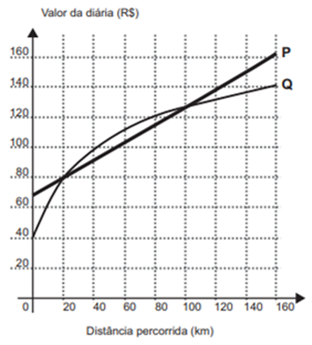
\includegraphics[width=180bp]{locadora}
\end{figure}


\begin{enumerate}

\item{}
Suponha que uma pessoa resolveu alugar um carro pela locadora $Q$ e pagou menos que 100 reais pelo valor da diária. Quais os valores possíveis para a distância que essa pessoa percorreu com o carro?

\item{}
Se um outro cliente alugar um carro, agora na locadora $P$ e pagar no mínimo 80 e no máximo 140 reais na diária do veículo, quais os possíveis valores para a distância percorrida com ele?

\item{}
Qual a locadora mais vantajosa, em termos de custo do aluguel, para uma pessoa que deseja alugar um carro para percorrer uma distância total de $80 km$?

\item{} Para quais valores da distância a ser percorrida de carro por uma pessoa, o custo do aluguel será o mesmo tanto para a locadora $P$ quanto para a $Q$?

\item{} Para quais valores da distância a ser percorrida de carro por uma pessoa, fica mais barato alugar o carro pela locadora $P$. E pela locadora $Q$? 

\end{enumerate}
\end{task}



\arrange{Inequações em uma incógnita}
\label{\detokenize{AF107-6:inequacoes}}\label{\detokenize{AF107-6::doc}}

O conceito de inequação em Matemática é motivado pelo estudo de \emph{desigualdades} entre duas ou mais grandezas. Problemas com desigualdades surgem naturalmente no dia a dia e costumam envolver as expressões "mais", menos", "maior do que"{} ou "menor do que". Por exemplo: quais os dias de 2019 em que a temperatura máxima no Rio de Janeiro foi maior que em Salvador? O desmatamento da Amazônia em 2018 foi menor que em 2020? Quais os dias do ano em que o preço da passagem do ônibus esteve mais barata que o preço do trem? Quais os meses do ano que a sua conta de luz custou mais que 150 reais? 

Em Matemática, os símbolos $"<"$ e $">"$ são usados para representar, respectivamente, os termos "menor do que"{} ou "maior do que". Dessa forma, quando escrevemos $3<5$ devemos ler: \emph{3 é menor do que 5}. Quando escrevemos $8 > 1$, lemos: \emph{8 é maior do que 1}.

Os símbolos $"\leq"$ (menor do que ou igual a) e $"\geq"$ (maior do que ou igual a) também são utilizados em problemas matemáticos envolvendo desigualdades.

Uma \emph{inequação}, assim como uma equação, também envolve duas expressões matemáticas envolvendo uma ou mais incógnitas, porém, essas expressões não se relacionam através de uma igualdade e sim através dos dos símbolos $>, \ <, \ \leq,\ \mbox{ou} \, \geq$. Por exemplo:
\begin{enumerate}
\item{}
$x^2 + 2x < 5 - x$;

\item{}
$a^2 \geq b^2 + c^2$;

\item{}
$\sqrt{mn} \leq \frac{m+n}{2}.$
\end{enumerate}

Quando atribuímos valores às incógnitas de uma inequação e obtemos uma desigualdade verdadeira, dizemos que esses valores compõem uma \emph{solução da inequação}. Na inequação a) acima, $x = 1$ é uma solução, pois quando substituímos $x$ por $1$, obtemos $2<4$ (2 é menor do que 4) o que é uma desigualdade verdadeira. Já $x = 2$ não é uma solução, pois substituirmos $x$ por $2$ obtemos $8<3$ (8 é menor do que 3), o que claramente é falso. Na inequação do item \titem{b)}, o terno de valores $a = 4$, $b=3$ e $c=1$ é uma solução, pois é verdade que $16\geq 10$ (16 é maior do que ou igual a 10). O mesmo vale para o terno $a = 5$, $b = 3$ e $c = 4$, visto que $25 \geq 25$ (25 é maior do que ou igual a 25).

Neste capítulo, vamos nos restringir ao estudo das inequações em uma única incógnita. O conjunto solução de uma inequação em uma incógnita $x$ é o total de valores do conjunto universo (onde se considera previamente onde incógnita pode assumir valores) que ao serem atribuídos a $x$, resultam numa desigualdade verdadeira.

Apesar de terem nomes parecidos, equações e inequações têm estratégias bem diferentes de resolução. Quando resolvemos a equação $x^2 = 25$, sabemos que há duas soluções: uma é a raiz quadrada de 25 e a outra, é o seu simétrico, pois dois números opostos sempre têm o mesmo quadrado. Logo,
$$
x = \pm \sqrt{25} \ \ \ \therefore x = 5 \ \ \mbox{ou} \ \ x = -5.
$$
Já na inequação $x^2 <25$, se tentássemos proceder de forma parecida ao exemplo de equação e simplesmente "passar a raiz quadrada", chegaríamos a $x < \pm \sqrt{25}$, e poderíamos imaginar que $x < 5$ ou $x < -5$. Como todo número menor do que $-5$ evidentemente é menor do que $5$, poderíamos escrever apenas que $x<5$ e achar que o conjunto solução da inequação $x^2 < 25$ era dado por:
$$
S = \{x \in \mathbb{R} \ | \ x <5\},
$$ 
porém, repare que $-6 < -5$, mas $-6$ \textbf{não é uma solução da inequação} $x^2 <25$, pois $(-6)^2 = 36$ é \textbf{maior} que $25$! Assim, não podemos simplesmente replicar para as inequações os mesmos procedimentos algébricos usados para resolver equações, pois eles podem flevar a conclusões erradas!



Como fazer então para resolver inequações corretamente? Na atividade \emph{\hyperref[locadora]{Locadora de Carros}} você comparou os valores dos preços oferecidos no aluguel de carros por duas locadoras. Ambos os preços variavam com o valor $x$ da distância percorrida pelo cliente. Assim, o preço do aluguel do carro da primeira locadora era dado por uma função $f$ e o da segunda, por uma função $g$, ambas dependentes da variável $x$. No item \titem{e)} daquela atividade, você determinou quais os valores de $x$ para os quais a primeira locadora é mais barata, o que se traduz matematicamente na seguinte inequação:
$$
f(x) < g(x).
$$
Portanto, você foi capaz de resolver essa inequação analisando os gráficos dessas duas funções! 

\def\currentcolor{session2}
\clearmargin
\begin{objectives}{Potência de uma Lâmpada}
{
\begin{itemize}
\item Representar graficamente um intervalo.
\item Compreender um intervalo como solução de desigualdades simultâneas.
\end{itemize}
}{1}{2}
\end{objectives}
\begin{sugestions}{Potência de uma Lâmpada}
{
Tranquilize seus alunos com relação aos valores dessa atividade. Eles podem achar que estão seguindo pelo caminho errado porque os valores encontrados não são números inteiros, no entanto, lembre-os que os valores encontrados na realidade são assim mesmo.
}{1}{2}
\end{sugestions}
\clearmargin
\begin{answer}{Potência de uma Lâmpada}
{
\begin{enumerate}
\item No eixo $Oy$ marque o intervalo $[116,133]$.
\item  Os valores aproximados de $P$ que correspondem às voltagens de $116V$ e $133V$ respectivamente são $93{,}4$ W e $122{,}8$W, assim, marque no eixo $Ox$  o intervalo $[93{,}4;122{,}8]$.
\end{enumerate}
}{1}
\end{answer}
\def\currentcolor{session4}
\begin{observation}{}
\textbf{Resolvendo Inequações Graficamente}

Considere, na imagem a seguir, as funções $f$ e $g$ e que $P_1$ e $P_2$ são os únicos pontos de interseção entre os seus gráficos.

\begin{figure}[H]
\centering
\noindent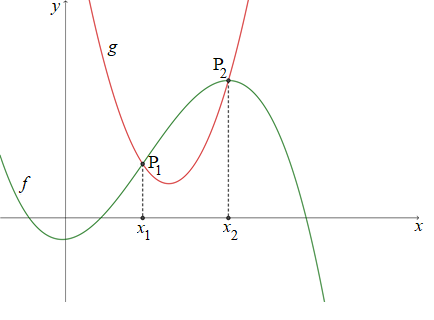
\includegraphics[width=300bp]{grafico_inequacao}
\end{figure}


\begin{enumerate}
\item{}
	Resolver a equação $f(x) = g(x)$, geometricamente, significa buscar os valores de $x$ (abscissas) dos pontos que pertençam, simultaneamente, aos gráficos das duas funções $f$ e $g$. Na figura acima, esses pontos são $P_1$ e $P_2$ e os valores de $x$ a eles associados são $x = x_1$ e $x = x_2$. Logo, o conjunto solução da equação $f(x) = g(x)$ é $S =\{x_1, x_2\}$.

\item{}	
Resolver a inequação $f(x) > g(x)$, geometricamente, significa buscar as abscissas dos pontos para os quais o valor da função $f$ seja  maior do que o da função $g$. Graficamente, em um valor $a$ fixado tem-se $f(a)>g(a)$ quando o ponto do gráfico de $f$ correspondente a $a$ está \textbf{acima} do ponto do gráfico de $g$ correspondente a $a$. Assim, a solução da inequação $f(x)>g(x)$ corresponde aos intervalos do eixo $x$ para os quais o gráfico de $f$ está \textbf{acima} do gráfico de $g$. Na figura acima, a solução consiste exatamente no intervalo aberto $]x_1, x_2[$. Note que os pontos $x_1$ e $x_2$ não são soluções pois neles, as duas funções coincidem. Também poderíamos denotar esse conjunto solução por $S = \{x \in \mathbb{R}\ | \ x_1 < x < x_2\}$.

\item{}
Resolver a inequação $f(x) < g(x)$, geometricamente, significa buscar as abscissas dos pontos para os quais o valor da função $f$ seja menor do que o da função $g$. Graficamente, em um valor $a$ fixado tem-se $f(a)<g(a)$ quando o ponto do gráfico de $f$ correspondente a $a$ está \textbf{abaixo} do ponto do gráfico de $g$ correspondente a $a$. Assim, a solução da inequação $f(x)<g(x)$ corresponde aos intervalos do eixo $x$ para os quais o gráfico de $f$ está \textbf{abaixo} do gráfico de $g$. Na figura acima, a solução consiste exatamente aos números reais que pertencem ao intervalo aberto $]-\infty, x_1[$ ou ao intervalo $]x_2, +\infty[$. Note que os pontos $x_1$ e $x_2$ não são soluções pois neles, as duas funções coincidem. Também poderíamos denotar esse conjunto solução por $S = \{x \in \mathbb{R}\ | x < x_1 \ \mbox{ou} \ x > x_2\}$.

\item{}
O conjunto solução $S$ da inequação $f(x) \leq g(x)$ equivale unir os conjuntos soluções da inequação $f(x) < g(x)$ e da equação $f(x) = g(x)$. Logo, $S$ é o intervalo fechado $[x_1, x_2]$. Também podemos escrever $S = \{x \in \mathbb{R}\ | \ x_1 \leq x \leq x_2\}$. O mesmo raciocínio vale para detemrinar o conjunto solução da inequação $f(x) \leq g(x)$.

\item{}
Resolver a inequação $f(x) < 0$ significa buscar os valores de $x$ nos quais a função $f$ é menor que zero, ou seja, é negativa. Note que nessa inequação, estamos comparando duas funções também, a saber, a função $f$ e uma função $h(x)=0$, cujo gráfico é o eixo dos $x$. Assim, , os valores de $x$ para os quais $f(x) <0$ estão nos intervalos do eixo $x$ para os quais o gráfico de $f$ está \textbf{abaixo} desse eixo (desconsiderando os valores de $x$ nos quais o gráfico está exatamente sobre o eixo $x$!). O raciocínio para o conjunto solução da inequação $f(x) >0$ é o mesmo, considerando agora os valores de $x$ para os quais o gráfico de $f$ está \textbf{acima} do eixo $x$.
\end{enumerate}

\end{observation}


\practice{Inequações em uma incógnita}
\label{\detokenize{AF107-6:inequacoes}}\label{\detokenize{AF107-6::doc}}


\begin{task}{Potência de uma Lâmpada}
As redes elétricas de alguns estados do Brasil são projetadas para receberem uma tensão de 127V (Volts), porém existe uma variação natural nesse valor. As concessionárias estipulam uma variação máxima entre 116V e 133V e todos equipamentos fabricados no país são testados para suportar essa variação de tensão. Oscilações maiores na rede elétrica podem comprometer a potência dos eletrodomésticos e até mesmo avariá-los.

A potência de uma lâmpada está relacionada à tensão da rede elétrica e à resistência da lâmpada. Em Física, verifica-se que essa relação se dá através da seguinte fórmula:
$$
V = \sqrt{P\cdot R},
$$
onde $P$ representa a potência da lâmpada, medida em \emph{Watts} (W), $V$ é a tensão da rede medida em \emph{Volts} (V) e $R$ é a resistência da lâmpada medida em \emph{Ohms} ($\Omega$). Suponha que uma lâmpada de quintal tenha uma resistência de 144$\Omega$. O gráfico de $V$ em função $P$ é dado na figura abaixo: 

\begin{figure}[H]
\centering
\noindent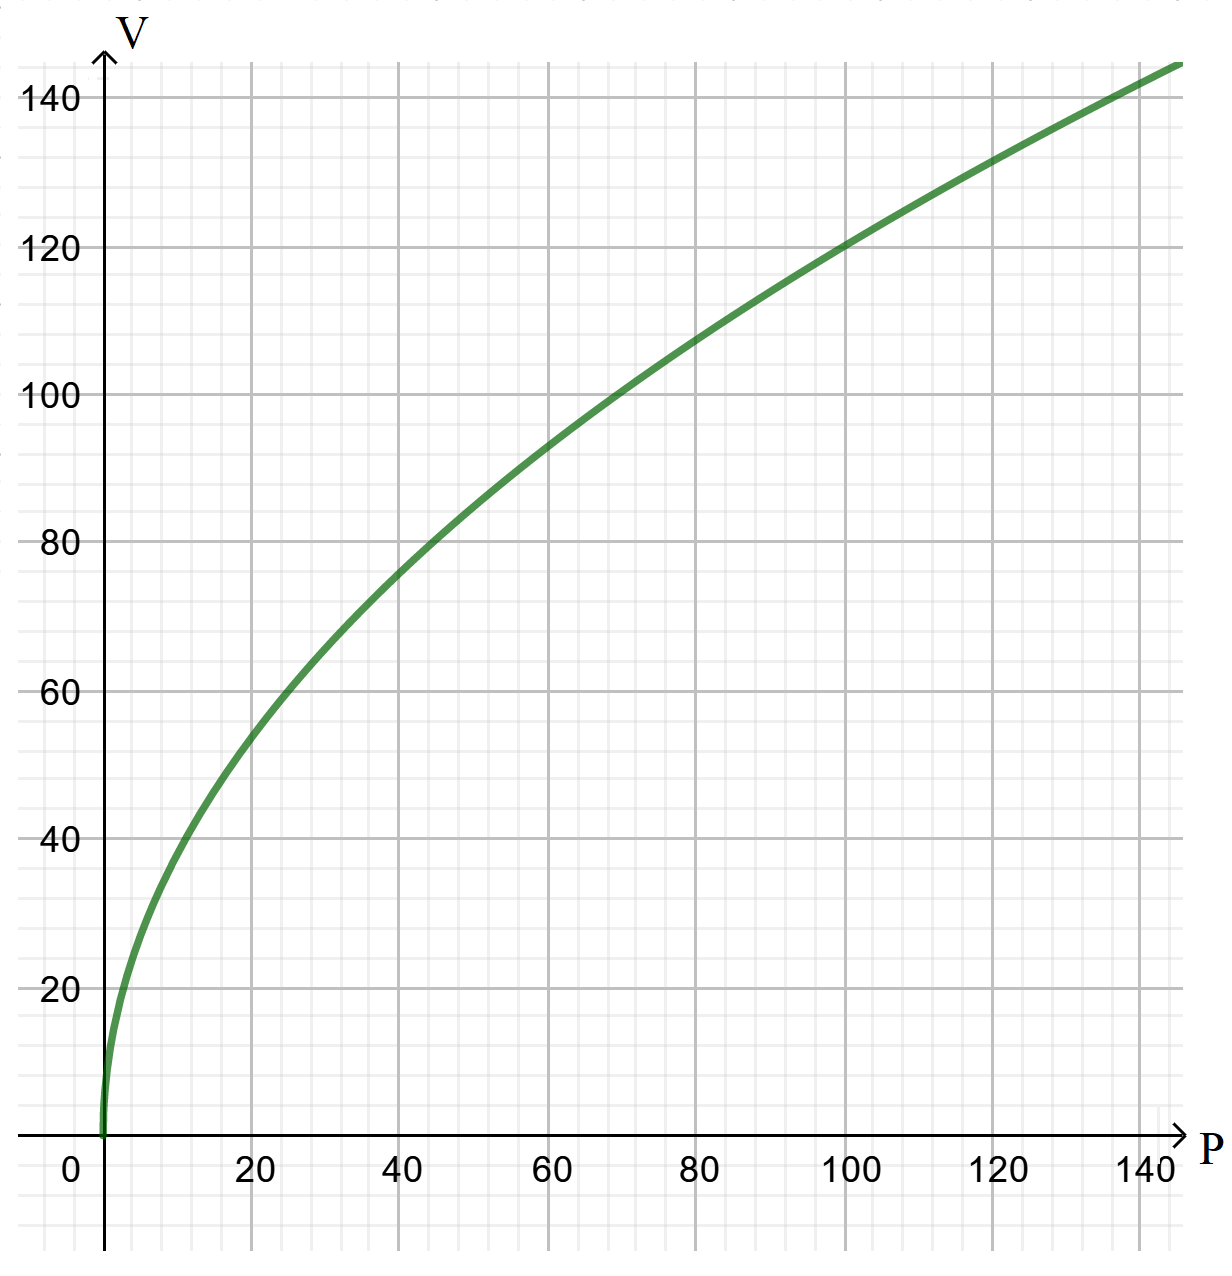
\includegraphics[width=200bp]{lampada}
\end{figure}

\begin{enumerate}
\item{}
Desenhe no eixo vertical o segmento que corresponde ao intervalo de variação de valores da tensão da rede estipuladas pelas concessionárias brasileiras.

\item{}
Desenhe no eixo horizontal, o segmento que corresponde ao intervalo de variação da potência da lâmpada, sabendo-se que a tensão $V$ oscila no intervalo $116\leq V \leq 133$. Em seguida, calcule o valor mínimo e máximo atingidos pela potência desta lâmpada.
\end{enumerate} 

\end{task}

\cleardoublepage

\def\currentcolor{session1}
\begin{objectives}{Estudando o sinal de uma função afim usando o GeoGebra}
{
\begin{itemize}
\item Estudar a variação do sinal de uma função afim. 
\item Estabelecer condições para que a função afim seja crescente ou decrescente.
\item Compreender o significado geométrico do sinal de uma função afim.
\end{itemize}
}{1}{1}
\end{objectives}
\begin{sugestions}{Estudando o sinal de uma função afim usando o GeoGebra}
{
Professor, essa é uma construção que contribuirá para que o aluno compreenda o significado do estudo da variação do sinal de uma função. É muito comum que o aluno confunda o sinal de $x$ com o sinal de $y$. Por essa razão, a construção do segmento orientado vai auxiliar a que ele perceba que, conforme $x$ cresce, a função tem seu sinal variando de acordo com a localização de sua raiz, de negativo para positivo, se a função for crescente, e de positivo para negativo, se a função for decrescente. Certifique-se de que o aluno sempre movimente o ponto livre construído no eixo $Ox$ para a esquerda ao máximo possível para iniciar sua observação. Você pode ainda sugerir que o estudante habilite o rastro do segmento orientado (vetor) construído, de forma que ele visualizará regiões sob/sobre o eixo dos $x$, enfatizando a variação do sinal. Veja como ficaria habilitando o rastro.
}{1}{1}
\end{sugestions}
\clearmargin
\begin{answer}{Estudando o sinal de uma função afim usando o GeoGebra}
{
\begin{enumerate}
\item Crescente.
\item Conforme o ponto $A$ avança do negativo para o positivo, o vetor  muda sua orientação de "apontando para baixo" para "apontando para cima", acompanhando o sinal da função (quando a função é negativa, ele aponta para baixo, quando ela é positiva, ele aponta para cima).
\item Decrescente.
\item Conforme o ponto $A$ avança do negativo para o positivo, o vetor  muda sua orientação de "apontando para cima" para "apontando para baixo", acompanhando o sinal da função.
\item o vetor $\overrightarrow{AB}$ alterna o seu sentido de cima para baixo exatamente quando o ponto $A$ se encontra sobre o zero da função afim.
\end{enumerate}
}{1}
\end{answer}
\explore{Inequações Polinomiais de Grau 1}
\label{\detokenize{AF107-7:inequacoes-grau1}}\label{\detokenize{AF107-7::doc}}

\begin{task} {Estudando o sinal de uma função afim com o GeoGebra}
Vamos fazer uma construção usando o GeoGebra. Siga os seguintes passos:
\begin{enumerate}
\item[(1)] 
Abra a janela gráfica e escreva $y=ax+b$ no campo de entrada e tecle ENTER
\end{enumerate}

\begin{figure}[H]
\centering
\noindent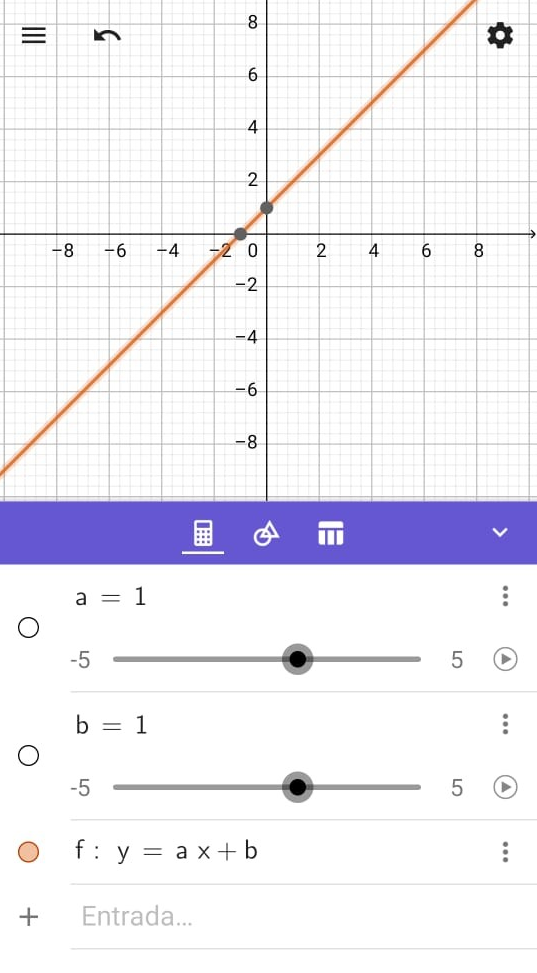
\includegraphics[width=200bp]{inequacaolinear}
\end{figure}

Observe que o GeoGebra denominou por $f$ a função que associa $x$ e $y$ por meio da expressão analítica $y=ax+b$ e gerou, automaticamente, dois controles deslizantes para os valores de $a$ e $b$, variando de $-5$ a $5$. Movimente os controles deslizantes e verifique o que ocorre com a função.


\begin{figure}[H]
\centering
\noindent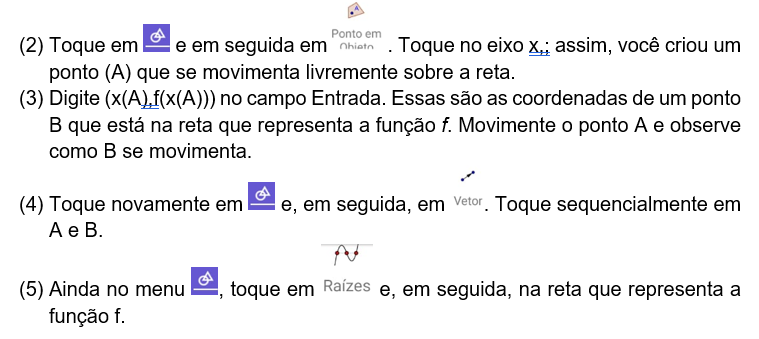
\includegraphics[width=400bp]{icones}
\end{figure}

Agora vamos explorar um pouco a sua construção?

\begin{enumerate}
\item{} 
Ajuste o controle deslizante $a$ para um valor maior que zero. A função $f$ exibida é crescente ou decrescente?

\item{}
 Ainda com o mesmo valor usado em \titem{a)}, movimente o ponto $A$ pelo eixo $x$, deslocando-o inicialmente para os valores mais negativos de $x$ que você consiga visualizar em sua tela. Agora, movimente lentamente o ponto $A$ para a direita, no sentido positivo do eixo $x$. o que você observa sobre o vetor $AB$?
 
\item{} 
Retorne o ponto $A$ para a esquerda do eixo $x$. Movimente o controle deslizante $a$ de forma que ele assuma um valor menor que zero. A função $f$ agora é crescente ou decrescente?

\item{}
Mantendo o mesmo valor para $a$ usado no item \titem{c)}, movimente lentamente o ponto $A$ no sentido positivo do eixo $x$. O que você observa em relação ao vetor $AB$?

\item{}
Como você pode relacionar a raiz da função (abscissa do ponto $C$) com o que você observou sobre o vetor $AB$ nos itens \titem{b)} e \titem{d)}?

\end{enumerate}
\end{task}

\arrange{Inequações Polinomiais de grau 1}
\label{\detokenize{AF107-7:inequacoes-grau1}}\label{\detokenize{AF107-7::doc}}

Inequações cujas expressões envolvem somas e diferenças de constantes ou de múltiplos constantes da incógnita $x$ são chamadas de \emph{Inequações Polinomiais de 1\super{o} grau}. Abaixo temos alguns exemplos de inequações polinomiais de 1\super{o} grau:

\begin{enumerate}
\item{}
$2x + 5 \geq 0$;

\item{}
$4x - 7 < 5 - 2x$;

\item{}
$13x + 8 \geq -6x$.
\end{enumerate}

Repare que as expressões que aparecem à esquerda ou à direita do sinal de desigualdade são dadas por funções afins ou funções constantes. Utilizando o que aprendemos na seção anterior, já é possível encontrar as soluções de todas essas inequações. Por exemplo, para resolver a inequação do item \titem{b)}, basta esboçarmos os gráficos das funções $f(x) = 4x -7$ e $g(x) = 5 - 2x$ e observarmos os valores de $x$ para os quais o gráfico de $f$ fica abaixo do gráfico de $g$:

\begin{figure}[H]
\centering
\noindent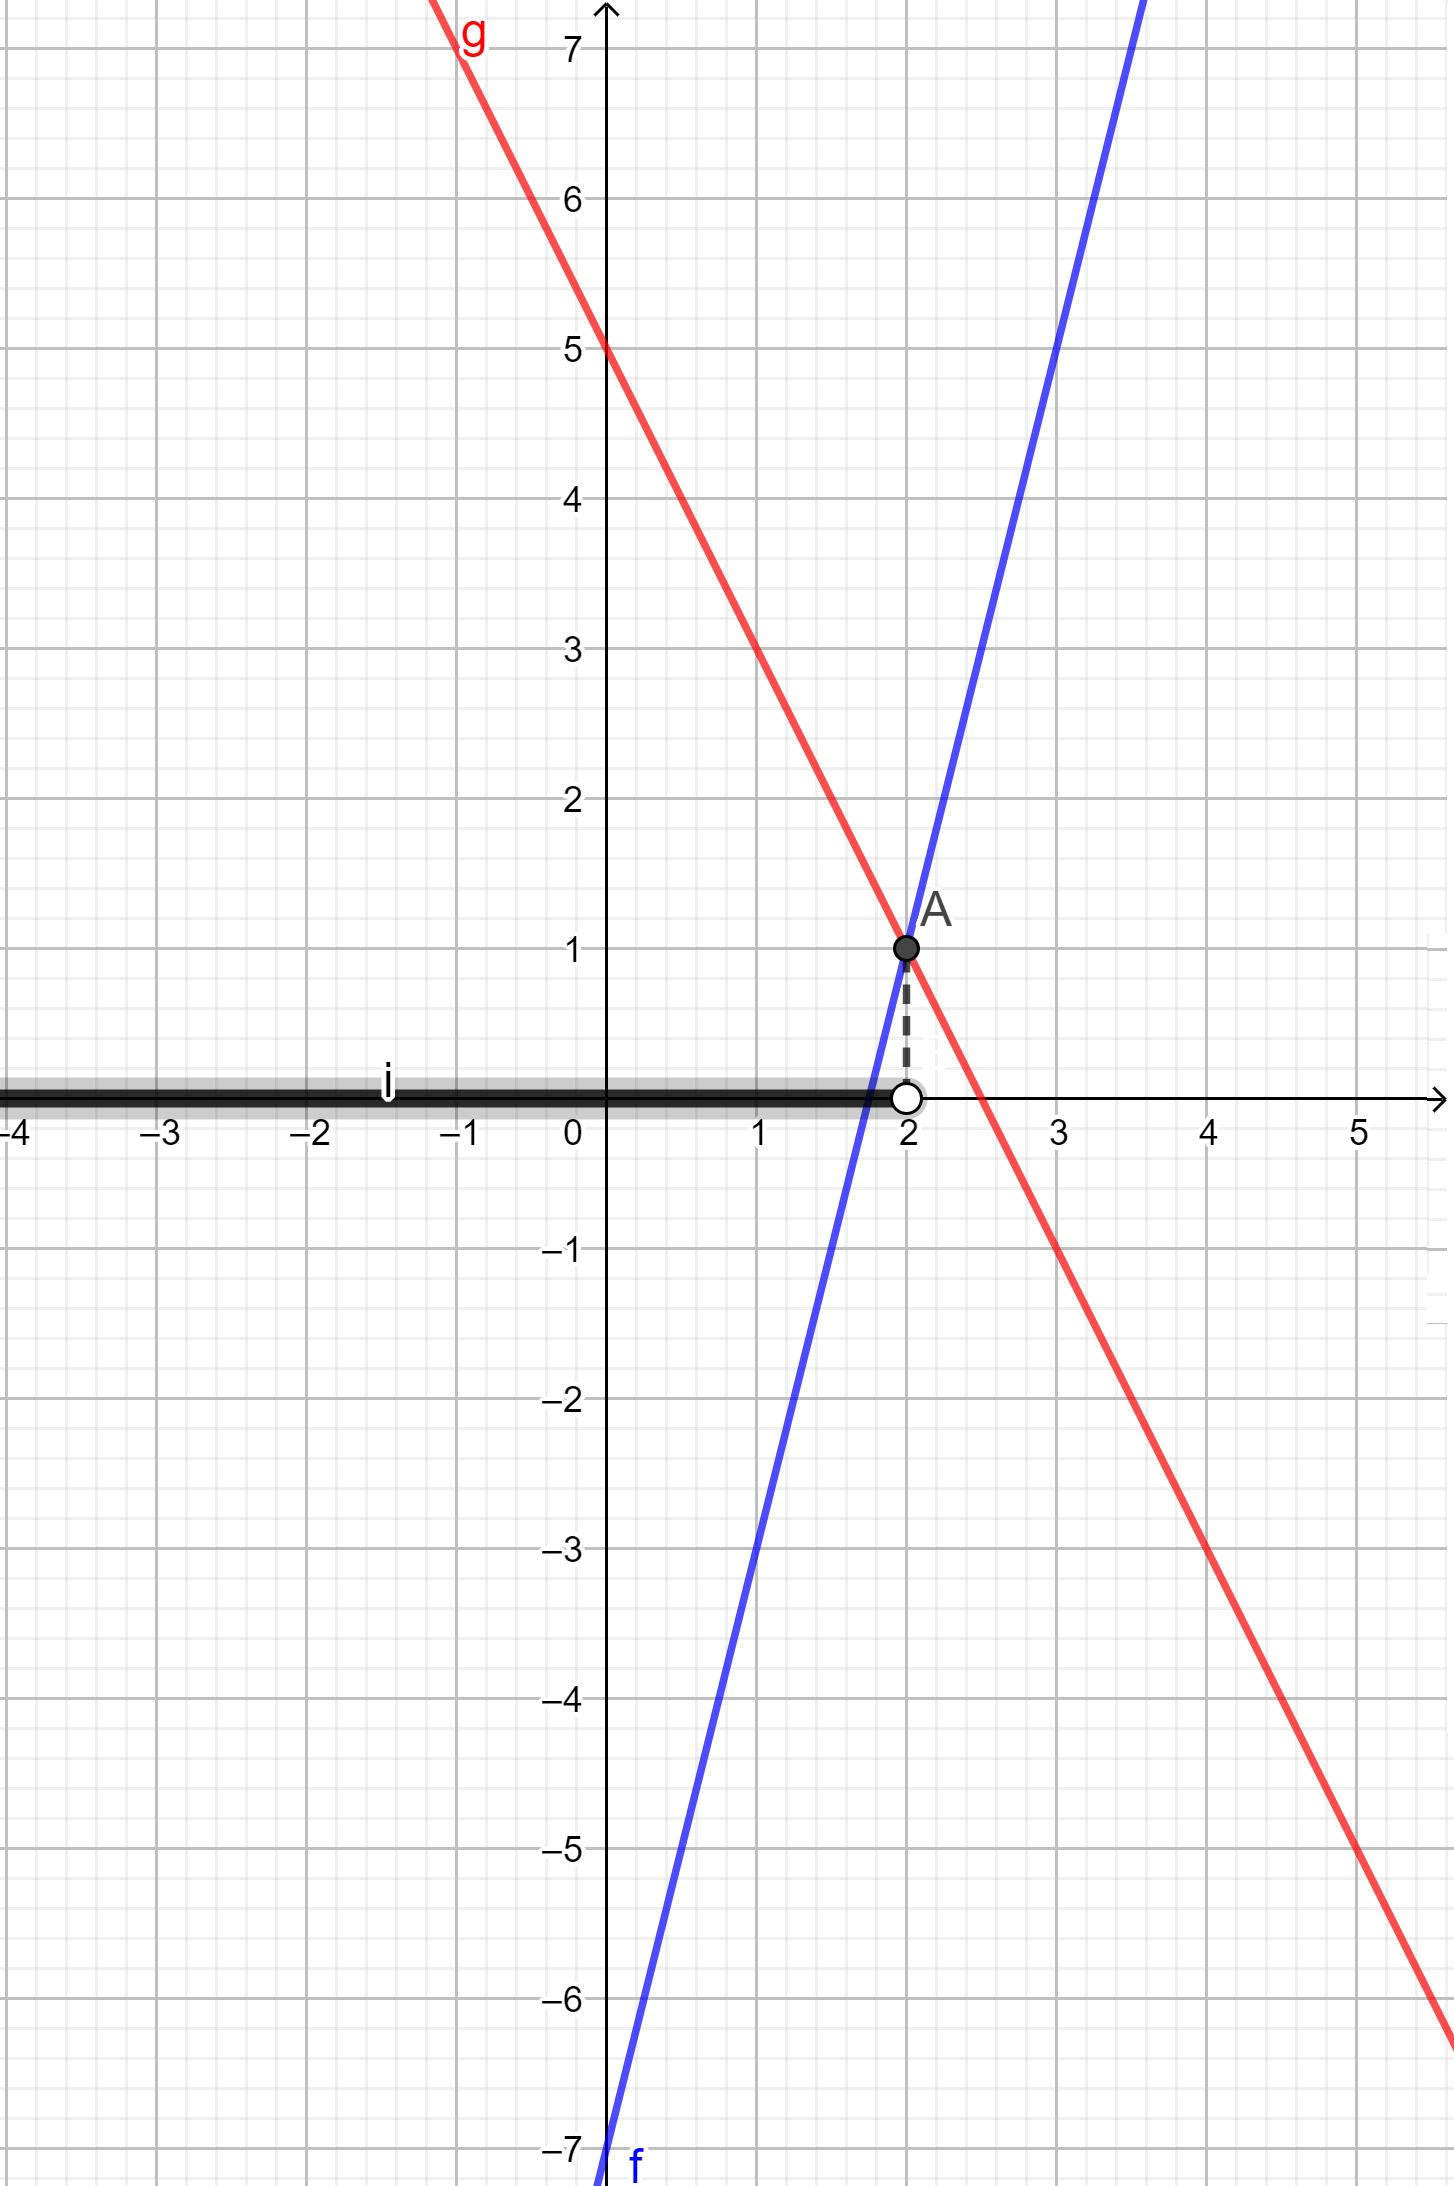
\includegraphics[width=200bp]{exemplo_inequacao1}
\end{figure}

Para encontrar a abscissa do ponto de interseção dos gráficos, basta resolver a equação $f(x) = g(x)$. Temos:
$$
f(x) = g(x) \ \iff \ 4x - 7 = 5 - 2x \ \iff \ 4x +2x = 5 +7 \ \iff 6x = 12 \ \therefore \ x = 2.
$$
Assim, os pontos do gráfico de $f$ estão abaixo dos de $g$ sempre que $x<2$. Portanto, o conjunto solução desta inequação é o intervalo $]-\infty, -2[$.

Estudaremos nessa seção uma maneira alternativa de se resolver inequações do 1\super{o} grau, que se resume a analisar o sinal da imagem de uma função afim. Consideremos uma função afim $f(x) = ax + b$. \emph{Estudar a variação do sinal} dessa função significa indicar para que valores de $x$ a função $f$ é positiva, para que valores é negativa e para que valor ela se anula. A resposta a essa questão vem a partir do estudo do seu gráfico, mas pode ser resumido a partir da análise da variação do crescimento da função e do valor de $x$ no qual ela se anula (\textbf{zero} da função $f$).

Lembre-se que a função afim $f(x) = ax + b$ se anula em um único valor, a saber, na solução da equação ax + b = 0, ou seja $x =  -\frac{b}{a}$.  Portanto, $(-\frac{b}{a},0)$ é ponto do gráfico de $f$, localizado sobre o eixo $x$. Como o gráfico da função afim é uma reta, esta irá intersectar o eixo $x$ precisamente no ponto $(-\frac{b}{a},0)$.


Vamos esboçar o gráfico dessa função, mas de maneira resumida, sintética - quase uma caricatura da função, focados em analisar o comportamento do sinal da imagem de $f$. Temos duas possibilidades: essa função pode ser crescente, se tivermos $a > 0$, ou decrescente, se tivermos $a < 0$.

\begin{figure}[H]
\centering
\noindent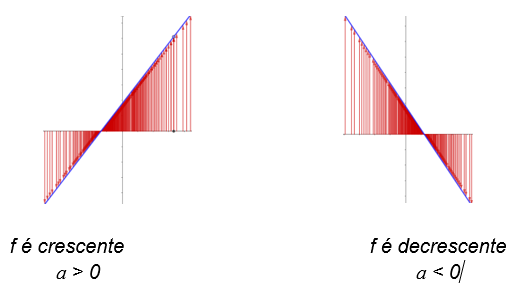
\includegraphics[width=300bp]{sinal_afim}
\end{figure}

Observe que quando $f$ é crescente, os valores de $x$ que se localizam à esquerda do zero da função (ou seja, $x < -\frac{b}{a}$) correspondem a pontos da reta que se localizam abaixo do eixo $x$, para os quais os valores das imagens $f(x)$ são negativos. Por outro lado, os valores de $x$ que se localizam à direita do zero da função (ou seja, $x > -\frac{b}{a}$)  correspondem a pontos da reta que se localizam acima do eixo $x$, para os quais os valores $f(x)$ das imagens são positivos.

De modo similar, quando $f$ é decrescente, os valores de $x$ que se localizam à esquerda do zero da função (ou seja, $x < -\frac{b}{a}$) correspondem a pontos da reta que se localizam acima do eixo $x$, para os quais os valores das imagens $f(x)$ são positivos. Por outro lado, os valores de $x$ que se localizam à direita do zero da função (ou seja, $x > -\frac{b}{a}$)  correspondem a pontos da reta que se localizam abaixo do eixo $x$, para os quais os valores $f(x)$ das imagens são negativos.

\begin{figure}[H]
\centering
\noindent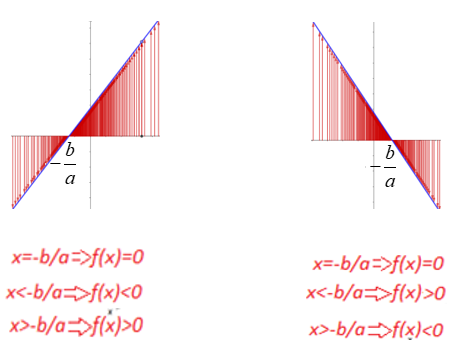
\includegraphics[width=300bp]{sinal_afim1}
\end{figure}

Uma propriedade que as desigualdades possuem, similar à da igualdade, é que ela se preserva quando somamos ou subtraímos um mesmo número real nas expressões à esquerda e à direita que a compõem, isto é:
$$
a < b \ \iff \ a + c < b +c. 
$$
Podemos nos convencer sobre esta propriedade interpretando-a na reta numérica: se $a < b$ então $a$ aparece na reta numérica à esquerda de $b$. Se somarmos um número $c$ ao número $a$, o efeito geométrico na reta será de uma translação de $|c|$ unidades do ponto $a$ para o ponto $a+c$, que será para a direita quando $c>0$ e que será para a esquerda quando $c <0$.

\begin{figure}[H]
\centering
\noindent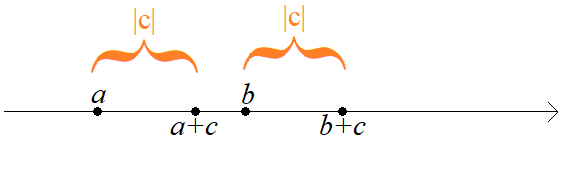
\includegraphics[width=300bp]{reta_numerica}
\end{figure}

Vamos retomar o exemplo da inequação $4x-7 < 5-2x$. Substraindo o número real $5$ nos dois termos da desigualdade, obtemos:
$$
4x-7 < 5 - 2x \ \iff \ 4x - 7 - 5 < 5 - 2x - 5 \ \iff \ 4x - 12 < - 2x,
$$
e agora, somando o número $2x$ em ambos os termos, concluímos que:
$$
4x - 7 < 5 - 2x \ \iff \ 6x -12 < 0, 
$$
ou seja, a desigualdade dada pela inequação $4x - 7 < 5 - 2x$ é equivalente à desigualdade $6x - 12 < 0$. Portanto, os valores de $x$ que são soluções da inequação $4x - 7 < 5 - 2x$ são exatamente os mesmos que estão no conjunto solução de $6x - 12 <0$. Dessa forma, \textbf{resolver a primeira inequação equivale a resolver a segunda}. Por sua vez, $6x - 12 < 0$ pode ser resolvida usando o estudo da variação do sinal da função afim $f(x) = 6x - 12$. O zero de $f$ é dado pela solução da equação $6x - 12 = 0$, logo $x = 2$. Como $f$ é crescente, o gráfico de $f$ fica:

   \begin{figure}[H]
\centering
\noindent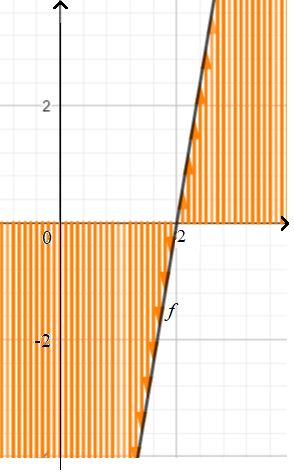
\includegraphics[width=130bp]{inequacao2}
\end{figure}

Como queremos $f(x) < 0$, a parte do gráfico que fica abaixo do eixo $x$ é exatamente aquele que fica sobre o intervalor $]-\infty, 2[$, portanto esse é o conjunto solução da inequação.

Com base no que fizemos, podemos enunciar o seguinte resultado:

\begin{observation}{}
\textbf{Teorema:} Toda inequação polinomial do 1\super{o} grau pode ser reduzida a uma inequação da forma $f(x) <0$, $f(x) > 0$, $f(x) \leq 0$ ou $f(x) \geq 0$, onde $f$ é uma função constante ou uma função afim.

\end{observation}

Vamos fazer mais um exemplo: resolveremos a inequação polinomial do 1\super{o} grau abaixo:
$$
x + 8(3x - 2) \leq 4 + \frac{5x}{3}.
$$
Primeiro vamos resolver a distribuitiva e reduzir a expressão à esquerda do sinal de desigualdade:
$$
x + 24x - 16 \leq \ 4 + \frac{5x}{3} \ \iff \ 25x - 16 \leq \ 4 + \frac{5x}{3}.
$$
Agora, vamos obter uma inequação equivalente cujo termo à direita do sinal de desigualdade seja zero. Para isso, basta subtrair das duas expressões o número $4 + \frac{5x}{3}$:
\begin{align*}
25x - 16 \leq \ 4 + \frac{5x}{3} \ &\iff \ 25x - 16 - (4 + \frac{5x}{3}) \leq \ 4 + \frac{5x}{3} - (4 + \frac{5x}{3}) \\
 & \iff \ 25x - 16 -4 - \frac{5x}{3} < 0 \\
 & \iff \ \frac{70x}{3} - 20 < 0. \\
\end{align*}
Basta analisar o sinal da função afim $f(x) = \frac{70x}{3} - 20$. Primeiro encontramos o zero dessa função:
$$
f(x) = 0 \ \iff \ \frac{70x}{3} - 20 = 0 \ \iff \ \frac{70x}{3} = 20 \ \iff \ 70x = 60 \ \iff \ x = \frac{6}{7}.
$$
Como queremos resolver $f(x) \leq 0$, a solução inclui tanto os valores de $x$ que anulam a função (ou seja, $x = \frac{6}{7}$)
como aqueles que correspondem à parte do gráfico que fica abaixo do eixo $x$ ($x < \frac{6}{7}$).

\clearpage
\def\currentcolor{session2}
\begin{objectives}{Comparando preços em \textit{Lan Houses}}
{
\begin{itemize}
\item Modelar matematicamente fenômenos usando funções afins. 
\item Resolver uma inequação do primeiro grau algebricamente.
\item Resolver uma inequação do primeiro grau geometricamente.
\end{itemize}
}{1}{1}
\end{objectives}
\begin{sugestions}{Comparando preços em \textit{Lan Houses}}
{
\begin{itemize}
\item Comente com os alunos sobre a importância de considerar o tempo em horas para estudar essa situação, por exemplo, $3$h$15$min são $3,25$ horas, e não $3,15$.
\item No itens \titem{a)} e \titem{b)} faça os alunos calcularem começarem a pensar em como poderiam generalizar esse cálculo.
\item Para responder o item \titem{e)} incentive seus aluno a construir os gráfico das funções encontradas nos itens \titem{c)} e \titem{d)} e lembre-os de que as \textit{Lan Houses} só ficam abertas por $12$ hrs. 
\item Faça com que os alunos entendam também que, responder quando a Mega-Conexão é mais barata que a Net-Ágil é equivalente a resolver a inequação $2x<5-x$ e que responder quando a Net-Ágil é mais barata que a Mega-Conexão é equivalente a resolver a inequação $2x>5-x$
\end{itemize}
}{1}{1}
\end{sugestions}
\begin{answer}{Comparando preços em \textit{Lan Houses}}
{
\begin{enumerate}
\item Net-Ágil: R\$ $8{,}25$, Mega-Conexão:  R\$ $6{,}25$.
\item  O custo na Net-Ágil é de  R\$ $11{,}17$ enquanto na Mega-Conexão é de R\$ $12{,}33$, portanto a Net-Ágil é a escolha mais econômica.
\item $f(x)=5+x$.
\item $g(x)=2x$.
\item De $1$ min a $5$ h, a melhor escolha é a Mega-Conexão. Entre $5$ e $12$ h, Net-Ágil.
\end{enumerate}
}{1}
\end{answer}
\clearmargin
\begin{objectives}{Elaborando um problema de inequações}
{
\begin{itemize}
\item Elaborar problemas envolvendo inequações de primeiro grau
\end{itemize}
}{1}{2}
\end{objectives}
\begin{sugestions}{Elaborando um problema de inequações}
{
Professor, nesse exercício, sugerimos que os alunos proponham os problemas em grupos e que troquem entre si. Cabe lembrar que a elaboração de problemas é uma habilidade enfatizada pela base nacional comum curricular e que estimula a criatividade e o vínculo entre objetos matemáticos e situações cotidianas para o aluno.
}{1}{2}
\end{sugestions}



\begin{figure}[H]
\centering
\noindent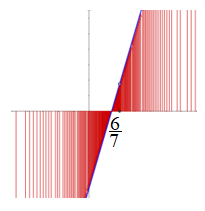
\includegraphics[width=175bp]{inequacao3}
\end{figure}

Portanto, a solução a inequação é $S = \{x \in \mathbb{R} \ | \ x \leq \frac{6}{7}\}$ ou então, usando a notação de intervalo, $S = ]-\infty, \frac{6}{7}]$.

\practice{Inequações Polinomiais de grau 1}
\label{\detokenize{AF107-7:inequacoes-grau1}}\label{\detokenize{AF107-7::doc}}

\begin{task}{Comparando preços em \emph{Lan Houses}}

Em alguns lugares onde é há baixo acesso à internet, ainda existem as \emph{Lan Houses}, que são estabelecimentos comerciais que ofertam serviço de internet para seus clientes usarem durante um certo período de tempo. A \emph{Lan house} Net-Ágil cobra 5 reais por acesso e mais 1 real por hora utilizada. Já na \emph{Lan House} Mega-Conexão, a cobrança é de 2 reais por hora. Ambas as Lan Houses cobram por frações de hora.

\begin{enumerate}
\item{}	
Se um cliente permanecer na \emph{Lan House} NetÁgil por 3h15min, qual será o valor a ser pago? E se escolher a \emph{Lan House} Mega-Conexão, quanto deverá pagar ao final desse período?

\item{}
Para usar os computadores e internet por 6h10min, qual das duas \emph{Lan House} seria a melhor escolha?

\item{}
Escreva a expressão algébrica que define a função $f$ e que retorna a cada tempo $x$ em horas o valor a ser pago em reais na \emph{Lan House} Net-Ágil.

\item{}	
Escreva a expressão algébrica que define a função $g$ e que retorna a cada tempo $x$ em horas o valor a ser pago em reais na \emph{Lan House} Mega-Conexão.

\item{}	
Suponha que as duas \emph{Lan Houses} funcionam das 8h às 20h. Para que valores de x a \emph{Lan House} Mega-Conexão é mais vantajosa?
\end{enumerate}

\end{task}

\begin{task}{Elaborando um problema de inequações}
Elabore problemas do seu cotidiano que sejam representados pelas inequações abaixo. Em seguida, resolva as inequações.
\begin{enumerate}
\item{}
$2x - 3 > 0$

\item{}
$4  - x < 1 + 8x$.
\end{enumerate}

\end{task}

\clearpage
\def\currentcolor{session1}
\begin{objectives}{Variação do Dólar}
{
\begin{itemize}
\item Aplicar as inequações do segundo grau em contextos de economia.
\item Compreender geometricamente uma inequação de segundo grau.
\item Resolver algébrica e geometricamente uma inequação do segundo grau.
\end{itemize}
}{1}{1}
\end{objectives}
\begin{sugestions}{Variação do Dólar}
{
Professor, lembre ao aluno que a variação do Dólar em relação ao Real é descrito pela função dada no exercício apenas nesse dia, portanto, ao responder ao item $c)$ ele deve atentar que que o tempo não pode ser negativo nem maior que $24$, pois ambos os casos representariam outros dias.
}{1}{1}
\end{sugestions}
\begin{answer}{Variação do Dólar}
{
\begin{enumerate}\setcounter{enumi}{1}
\item A partir das $0$hrs até às $15$hrs.
\item A partir das $15$hrs até o fim do dia.
\item O item $b)$ é representado por $f(t)=-0.002t^2-0.3t>0.$ O $c)$ fica $f(t)=-0.002t^2-0.3t<0. $
\end{enumerate}
}{1}
\end{answer}
\clearmargin
\begin{objectives}{Estudando o sinal de uma função quadrática com o GeoGebra}
{
\begin{itemize}
\item Associar o geogebra ao estudo da variação do sinal de funções quadráticass.
\end{itemize}
}{1}{2}
\end{objectives}
\begin{sugestions}{Estudando o sinal de uma função quadrática com o GeoGebra}
{
Nessa atividade, o objetivo é que o aluno perceba como varia o sinal da função quadrática.
Oriente seus alunos a que reproduzam os itens \titem{a)}, \titem{b)} e \titem{c)} dessa atividade para os casos em que $a>0$ e $\Delta =0, a>0$ e $\Delta <0, a<0$ e $\Delta>0, a<0$ e $\Delta=0, a<0$ e $\Delta<0$.
}{1}{2}
\end{sugestions}
\clearmargin
\begin{answer}{Estudando o sinal de uma função quadrática com o GeoGebra}
{
\begin{enumerate}
\item Para cima.
\item Positivo.
\item O vetor $AB$ alterna o seu sentido de cima para baixo exatamente quando o ponto $A$ passa pelo primeiro zero da função quadrática e depois de baixo para cima quando passa pelo segundo zero da função quadrática.
\end{enumerate}
}{1}
\end{answer}

\explore{Inequações Polinomiais de Grau 2}
\label{\detokenize{AF107-8:inequacoes-grau2}}\label{\detokenize{AF107-8::doc}}

\begin{task}{Variação do Dólar}
A cotação cambial do Dólar é um importante atributo para qualquer país e impacta vários indicadores econômicos, como inflação, balança comercial, dívida externa entre outros. 

\begin{figure}[H]
\centering
\noindent\includegraphics[width=200bp]{dolar}
\end{figure}

Suponha que em um determinado dia, a variação percentual $y$ do Dólar, frente o Real, tenha sido descrita pela seguinte função:
$$
y = -0,02t^2 + 0,3t, \ \ \ 9 \leq t \leq 17, 
$$
onde $t$ é medido em horas. Quando a variação percentual do Dólar é positiva, a moeda americana está se valorizando em relação ao Real, enquanto que quando esta variação é negativa, o dólar está se desvalorizando em relação ao Real.

\begin{enumerate}

\item{} Faça um esboço do gráfico da função $y = f(t)$ que descreve a variação percentual do dólar em função do tempo, no dia informado no enunciado;

\item{} Em qual período desse dia o dólar se valoriza em relação à nossa moeda? 

\item{} Em qual período desse dia o dólar se desvaloriza em relação ao Real?

\item{} Escreva algebricamente as perguntas dos itens \titem{b)} e \titem{c)};

\end{enumerate}

\end{task}


\clearpage
\begin{task}{Estudando o sinal de uma função quadrática com o GeoGebra}
Vamos fazer uma construção usando o GeoGebra. Siga os seguintes passos:

1-	Abra a janela gráfica e escreva $y=a(x-p)^2+q$ no campo de entrada e tecle ENTER;

\begin{figure}[H]
\centering
\noindent\includegraphics[width=175bp]{inequacao4}
\end{figure}

Observe que o GeoGebra denominou por $f$ à função que associa $x$ e $y$ por meio da lei algébrica $y=a(x-p)^2+q$ e gerou, automaticamente, três controles deslizantes para os valores de $a$, $p$ e $q$, variando de $-5$ a $5$. Movimente os controles deslizantes e verifique o que ocorre com a função. Quais os significados geométricos, na parábola, dos parâmetros $a$, $p$ e $q$?

\begin{figure}[H]
\centering
\noindent\includegraphics[width=400bp]{icones2}
\end{figure}
Agora vamos explorar um pouco a sua construção?

\begin{enumerate}
\item{} Ajuste o controle deslizante $a$ para um valor maior que zero. Como está a concavidade da função $f$?

\item {} Mantenha o controle deslizante $a$ fixo com o valor usado no item \titem{a)}. Arraste o ponto $A$ para o canto mais esquerdo do eixo $x$ e ajuste os controles $p$ e $q$ de forma que tenhamos duas raízes para a função $f$. Qual o sinal do discriminante $\Delta$?

\item{}	
Movimente lentamente o ponto $A$ no sentido positivo do eixo $x$. O que você observa sobre o vetor $\overrightarrow{AB}$? Descreva a posição desse vetor de acordo com as raízes da função $f$.
\end{enumerate}

\end{task}

\arrange{Inequações Polinomiais de grau 2}
\label{\detokenize{AF107-8:inequacoes-grau2}}\label{\detokenize{AF107-8::doc}}
Nesta seção, estamos estudando as chamadas \emph{inequações polinomiais de grau 2}. Tais inequações são aquelas cujas expressões algébricas envolvem somas de constantes ou de múltiplos constantes da incógnita ou do seu quadrado. Abaixo temos alguns exemplos de inequações polinomiais de 2\super{o} grau:

\begin{enumerate}
\item{}
$2x^2 + 4x \leq 5 - 4x$;

\item{}
$4 - \frac{\sqrt{3} \cdot x}{2} \geq -x^2$;

\item{}
$5x - 2x^2 > 1$.
\end{enumerate}

Utilizando o argumento, visto na seção anterior, de somar um mesmo número real nas duas expressões de uma desigualdade, podemos concluir o seguinte resultado:
 
\begin{observation}{}
\textbf{Teorema:} Toda inequação polinomial do 2\super{o} grau pode ser reduzida a uma inequação da forma $f(x) <0$, $f(x) > 0$, $f(x) \leq 0$ ou $f(x) \geq 0$, onde $f$ é uma função constante, afim ou quadrática.

\end{observation}

Para resolver qualquer inequação polinomial do 2\super{o} grau, aprenderemos a fazer o estudo do sinal de uma função quadrática.

Vamos considerar uma função quadrática $f(x) = ax2 + bx + c$ cujos zeros podem ser determinados por meio da fórmula:
$$
x = \frac{-b \pm \sqrt{\Delta}}{2a}.
$$  
Como vimos nos Capítulo de Função Quadrática, quando:

\begin{itemize}
\item  $\Delta >0$ $\Rightarrow$ $f$ tem exatamente dois zeros distintos;

\item   $\Delta =0$ $\Rightarrow$ $f$ tem um único zero;

\item  $\Delta <0$ $\Rightarrow$ $f$ não possui zeros.
\end{itemize}

Além disso, a concavidade do gráfico (parábola) é determinada pelo valor do coeficiente $a$: se  $a>0$, então a parábola apresenta concavidade voltada para cima; se $a<0$, então a parábola tem concavidade voltada para baixo. 


O estudo da variação do sinal de uma função quadrática é feito a partir do esboço de seu gráfico, considerando a posição da parábola que a representa em relação ao eixo $x$. Vamos ver alguns casos?


\begin{itemize}


\item[(1\super{o} caso:)] Se $a>0$, o gráfico de $f$ tem concavidade voltada para cima, e daí temos três possibilidades: ou a parábola está localizada totalmente acima do eixo $x$, ou ela intersecta o eixo $x$ em exatamente um ponto ou então intersecta o eixo dos $x$ em dois pontos. Lembramos que, no primeiro caso temos $\Delta <0$ , no segundo $\Delta = 0$   e no terceiro, $\Delta >0$. Portanto, no primeiro caso, os valores da função $f$ são positivos para todo $x$; no segundo caso, $f$ é positiva para todos os valores de $x$, exceto no seu zero (que corresponde ao ponto onde a parábola "toca"{} o eixo $x$) e no terceiro caso, se $x_1$ e $x_2$ são os seus zeros, $x_1<x_2$, então $f$ se anula nesses dois valores, $f(x)$ é negativa para $x_1 < x < x_2$ (sobre esse intervalo a parábola fica abaixo do eixo $x$) e $f(x)$ é positiva para $x<x_1$ e $x> x_2$ (sobre esses intervalos a parábola fica acima do eixo $s$).


\end{itemize}

\begin{figure}[H]
\centering
\noindent\includegraphics[width=400bp]{sinalquadratica}
\end{figure}

\begin{itemize}
\item[\textcolor{white}{............} (2\super{o} caso)] Se $a<0$, o gráfico de $f$ tem concavidade voltada para baixo, e daí temos três possibilidades: ou a parábola está localizada totalmente abaixo do eixo $x$, ou ela intersecta o eixo $x$ em exatamente um ponto ou então intersecta o eixo $x$ em dois pontos. No primeiro caso, os valores da função $f$ são negativos para todo $x$; no segundo caso, $f$ é negativa para todos os valores de $x$, exceto no seu zero (que corresponde ao ponto onde a parábola "toca"{} o eixo $x$) e no terceiro caso, se $x_1$ e $x_2$ são os seus zeros, $x_1<x_2$, então $f$ se anula nesses dois valores, $f(x)$ é positiva para $x_1 < x < x_2$ (sobre esse intervalo a parábola fica acima do eixo $x$) e $f(x)$ é negativa para $x<x_1$ e $x> x_2$ (sobre esses intervalos a parábola fica abaixo do eixo $x$). Construa as posições dos gráficos correspondentes a esse caso!


\end{itemize}
Vamos agora aplicar o estudo do sinal da função quadrática para resolver algumas inequações:

\vspace{0,2 cm}

\textbf{Exemplo 1:} Resolva a inequação $-x^2 \ \leq \ x - 12$.

Primeiramente, vamos obter uma desigualdade equivalente onde o termo à direita do sinal "$\leq$"{} seja igual a zero. Para isso, basta somar $(-x + 12)$ nos dois lados da inequação:
$$
-x^2 + (-x+ 12)\  \leq \ x - 12 + (-x+12) \ \iff \ -x^2 - x + 12 \leq 0.
$$
Basta então resolver a inequação $-x^2 - x +12 \leq 0$. Para isso, analisaremos o sinal da função quadrática $f(x) = -x^2 -x +12$. Ela tem dois zeros, a saber, $x_1 = -4$ e $x_2 = 3$ e a concavidade de seu gráfico é voltada para baixo, pois o coeficiente de $x^2$ é negativo. Agora, podemos organizar o desenho da análise do sinal de $f$:

\begin{figure}[H]
\centering
\noindent\includegraphics[width=150bp]{inequacao5}
\end{figure}

Como queremos resolver $f(x) \leq 0$ as soluções são dadas tanto pelos valores de $x$ que anulam $f$ como também por aqueles que correspondem aos pontos do gráfico que ficam abaixo do eixo $x$. Portanto, esses valores são exatamente aqueles que estão à esquerda de $-4$ ou à direita de $3$, incluindo esses dois números. Logo:
$$
S = \{x \in \mathbb{R}\ | \ x\leq -4 \ \mbox{ou} \ x \geq 3\ \}.
$$ 
Repare que o conjunto solução é dado por uma união de intervalos. Podemos escrever
$$
S = ]-\infty , -4] \cup [4, +\infty[.
$$

\vspace{0,2 cm}

\textbf{Exemplo 2:} Resolva a inequação $(x-2)^2 + 4 > 2(x-\frac{1}{2})$.

Vamos desenvolver as expressões nos dois lados da inequação:
$$
(x-2)^2 + 4 > 2(x-\frac{1}{2}) \ \ iff x^2 - 4x + 4 + 4 > 2x - 1 \ \iff \ x^2 - 4x + 8 > 2x - 1.
$$
Somando $-2x +1$ nas duas expressões da inequação, conseguimos reduzi-la a:
$$
x^2 - 4x + 8 + (-2x+1) > 2x - 1 + (-2x+1) \ \iff \ x^2 -6x + 9 > 0.
$$
Escrevendo $f(x) = x^2 - 6x + 9$, devemos resolver a inequação $f(x) > 0$. Para isso, analisamos o sinal de $f$. Esta função possui apenas $x = 3$ como zero e a concavidade do seu gráfico é voltada para cima, pois o coeficiente de $x^2$ é positivo. Portanto, o desneho da análise de sinal de $f$ é:

\clearpage
\def\currentcolor{session2}
\begin{objectives}{Concentração de álcool no sangue}
{
\begin{itemize}
\item Contextualizar uma inequação do segundo grau.
\end{itemize}
}{1}{2}
\end{objectives}
\begin{sugestions}{Concentração de álcool no sangue}
{
\begin{itemize}
\item Professor, faça o aluno perceber que a desigualdade apresentada aqui não é mais do tipo $ax^2+bx+c>0$ c mas do tipo $ax^2+bx+c>d$.
\item Tranquilize seus alunos com relação aos valores dessa atividade. Eles podem achar que estão seguindo pelo caminho errado porque estão acostumados a valores inteiros, no entanto, lembre-os que os valores encontrados em situações reais são assim mesmo.  
\end{itemize}
}{1}{2}
\end{sugestions}
\begin{answer}{Concentração de álcool no sangue}
{
Sim. A inequação base do problema é $-0{,}008(t^2-35t + 34)>1.$ A solução para ela é o intervalo $(5{,}35;29{,}65)$. Calculando a diferença temos $24{,}3$, portanto, superior a $23$ hrs
}{1}
\end{answer}
\begin{figure}[H]
\centering
\noindent\includegraphics[width=150bp]{inequacao6}
\end{figure}
O conjunto solução da inequação $f(x) > 0$, consiste em todos os valores de $x$ sobre os quais o gráfico de $f$ fica acima do eixo $x$, o que ocorre para qualquer número real exceto $x = 3$, onde o gráfico intersecta o eixo $x$ (isto é, $f$ se anula em $x = 3$). Portanto, o conjunto solução dessia inequação é:
$$
S = \{x \in \mathbb{R} \ | \ x \neq 3\ \} = \mathbb{R} - \{3\}.
$$

\practice{Inequações Polinomiais de grau 2}
\label{\detokenize{AF107-8:inequacoes-grau2}}\label{\detokenize{AF107-8::doc}}

\begin{task}{Concentração de álcool no sangue}
\textit{(Adaptada de Cespe - PRF)}

Considere que o nível de concentração de álcool na corrente sanguínea, em $g/L$, de uma pessoa, em função do tempo $t$, em horas, seja expresso por $N =-0{,}008(t^2 - 35t + 34)$. Considere, ainda, que essa pessoa tenha começado a ingerir bebida alcoólica a partir de $t = t_0$ ($N(t_0) = 0$), partindo de um estado de sobriedade, e que tenha parado de ingerir bebida alcoólica em $t = t_1$, voltando a ficar sóbria em $t = t_2$. Considere, por fim, a figura a seguir, que apresenta o gráfico da função $N(t)$ para $t \in [t_0, t_2]$. 


\begin{figure}[H]
\centering
\noindent\includegraphics[width=250bp]{alcool}
\end{figure}

Com base nessas informações e tomando $24{,}3$ como valor aproximado de $\sqrt{589}$, analise a afirmativa a seguir:

“O nível de concentração de álcool na corrente sanguínea da pessoa em questão foi superior a $1 g/L$ por pelo menos $23$ horas.”
\end{task}

\cleardoublepage
\def\currentcolor{session1}
\begin{sugestions}{Inequações produto ou quociente de funções de grau 1}
{
Caro professor, nessa atividade, esperamos que o estudante faça uma retomada das atividades introdutórias ao estudo das inequações de 1º e de 2º graus. Não desejamos recorrer apenas e diretamente às manipulações algébricas e memorizações de regras; esperamos que os alunos compreendam que resolver inequações que são obtidas por produtos ou quocientes entre funções afins ou quadráticas são resolvidas a partir da análise do sinal do produto/quociente dos fatores/termos. 
}{1}{1}
\end{sugestions}
\begin{answer}{Inequações produto ou quociente de funções de grau 1}
{\begin{enumerate}
\item A raiz de $f$ é $-2$ e de $g$ é $1$.
\item O sinal da função $f$ é negativo para valores menores que  $x=-2$, positivo valores maiores que $x=-2$ e nulo em $x=-2$;  a função $g$ é negativa para valores de $x$ menores que $1$; positiva para valores de $x$ maiores que $1$ e nula em $x = 1$.
\end{enumerate}
}{1}
\end{answer}
\clearmargin
\clearmargin
\begin{answer}{Inequações produto ou quociente de funções de grau 1}
{\begin{enumerate}\setcounter{enumi}{2}
\item Podem ambos estar abaixo do eixo $x$, ambos acima do eixo $x$ ou um abaixo e outro acima do eixo $x$.
\item Estão ambos abaixo do eixo $x$ para valores de $x$ menores que $-2$, raiz de $f$.
\item Estão ambos acima do eixo $x$ para valores de $x$ maiores que $1$, raiz de $g$.
\item Estão em sentidos opostos quando $x$ está entre $-2$ e $1$; aqui, $AB$ está acima do eixo $x$ (positivo) e $AC$ está abaixo do eixo $x$ (negativo).
\item Nesse caso, temos que o sinal de $h$ será positivo para valores de $x$ menores que $-2$ e para valores de $x$ maiores que $1$, pois nesse caso, o sinal das duas funções é o mesmo. Já quando $x$ é um valor entre $-2$ e $1$, o sinal de $h$ será negativo, pois nesse caso temos $f$ negativa e $g$ positiva. Em $x = -2$ ou em $x = 1$, como um dos fatores seria nulo, então temos que $h$ é nula.
\item Nesse caso, a situação é análoga ao item anterior, exceto pelo caso em que temos $x=1$ pois, nessa situação, $g(x)=0$, o que inviabiliza o quociente. Portanto, temos que $q$ é negativa quando $x$ está entre $-2$ e $1$ e positiva para valores de $x$ menores que $-2$ ou maiores que $1$. Em $x=-2, q$ será nula, pois teremos o quociente entre zero e um número negativo, o que resulta em zero.
\item Conforme vimos no item $(g)$, a função $h$ é negativa, estritamente, quando $x$ está entre $-2$ e $1$; logo, o conjunto solução dessa inequação é $]-2,1[$.
\item  Conforme vimos no item $(h)$ a função $q$ é positiva quando $x$ é menor que $-2$ ou quando $x$ é maior que $1$. No entanto, note que aqui a desigualdade está incluindo o zero; mas como precisaremos excluir o valor $1$ do domínio de $q$, então a solução será $]-\infty, -2]\cup ]1,+\infty[$
\end{enumerate}
}{1}
\end{answer}


\explore{Inequações Produto e Quociente}


\begin{task}{Inequações produto ou quociente de funções de grau 1}
Usando o GeoGebra, vamos plotar o gráfico das seguintes funções:
\begin{enumerate}[label=\titem{\roman*)}]
\item $y=2x+4$
\item $y=x-1$
\end{enumerate}

O GeoGebra denominará automaticamente essas duas funções por $f$ e $g$, respectivamente.

\begin{figure}[H]
\centering

\includegraphics[width=150bp]{inequacoes1}
\end{figure}


\begin{enumerate}
\item Quais são as raízes de $f$ e de $g$?
\item Descreva a variação do \textit{sinal} dessas duas funções. 
\end{enumerate}

Toque em \includegraphics[height=.75cm]{inequacoes32} e em seguida em \includegraphics[height=.75cm]{inequacoes33}. Toque no eixo $x$, assim, você criou um ponto $(A)$ que se movimenta livremente sobre o eixo $x$.

Digite no campo entrada $(x(A),f(x(A)))$ e $(x(A),g(x(A)))$. O GeoGebra nomeará, automaticamente, esses pontos como $B$ e $C$.

\begin{figure}[H]
\centering

\includegraphics[width=150bp]{inequacoes2}
\end{figure}

Toque novamente em \includegraphics[height=.75cm]{inequacoes32} e, em seguida, em \includegraphics[height=.75cm]{inequacoes34}. Toque sequencialmente em $A$ e $B$ e, em seguida, em $A$ e $C$, criando os segmentos orientados $\overrightarrow{AB}$ e $\overrightarrow{AC}$. 

\begin{figure}[H]
\centering

\includegraphics[width=150bp]{inequacoes3}
\end{figure}

Em seguida, ainda no menu  \includegraphics[height=.75cm]{inequacoes32}, toque em \includegraphics[height=.75cm]{inequacoes35} e, em seguida, em cada uma das duas retas que representam as funções $f$ e $g$, nessa ordem. Na tela você verá os pontos $E$ e $F$, raízes das funções $f$ e $g$, respectivamente.

\begin{figure}[H]
\centering

\includegraphics[width=150bp]{inequacoes4}
\end{figure}

\begin{enumerate}\setcounter{enumi}{2}
\item Movimente o ponto $A$ e descreva as possíveis posições relativas de $\overrightarrow{AB}$ e $\overrightarrow{AC}$
\item Em que intervalos $\overrightarrow{AB}$ e $\overrightarrow{AC}$ estão ambos abaixo do eixo $x$ (ou seja, para que valores de $x$ as funções $f$ e $g$ são negativas)?
\item Em que intervalos $\overrightarrow{AB}$ e $\overrightarrow{AC}$ estão ambos acima do eixo $x$ (ou seja, para que valores de $x$ as funções $f$ e $g$ são negativas)?
\item Em que intervalos $\overrightarrow{AB}$ e $\overrightarrow{AC}$ estão em sentidos opostos (ou seja, uma é positiva e outra é negativa)?
\item Vamos considerar agora a função $h(x) = f(x) \cdot g(x)$. Qual será o sinal de $h(x)$ quando $x < - 2$? E quando $x > 1$? E quando $-2 < x < 1$? E quando $x = -2$ ou $x = 1$? 
\item Faça o mesmo tipo de análise conduzida no item anterior para a função $q(x)=\dfrac{f(x)}{g(x)}$. 
\item A partir do que você percebeu acima (e sem desenvolver o produto), responda: qual a solução da inequação $f(x)\cdot g(x)<0$?
\item E qual a solução da inequação $\dfrac{f(x)}{g(x)}\geq0$ ? Os valores $x=-2$ e $x=1$ estão no conjunto solução dessa inequação? Justifique sua resposta.
\end{enumerate}
\end{task}

\arrange{Inequações Produto e Quociente}

Vamos considerar duas funções $f$ e $g$ quaisquer na variável $x$. As inequações $f(x)\cdot g(x)<0$, $f(x)\cdot g(x)>0$, $f(x)\cdot g(x)\leq0$ ou $f(x)\cdot g(x)\geq0$ são denominadas \textit{inequações-produto}. Da mesma forma, as inequações $\dfrac{f(x)}{g(x)}<0$, $\dfrac{f(x)}{g(x)}>0$, $\dfrac{f(x)}{g(x)}\leq0$ ou $\dfrac{f(x)}{g(x)}\geq0$ são denominadas \textit{inequações-quociente}.

A resolução de uma inequação-produto ou de uma inequação quociente pode ser determinada a partir do estudo conjunto da variação do sinal dos termos envolvidos no produto ou no quociente em questão, tomando como parâmetros de análise as raízes dessas funções.

Vamos ver alguns exemplos?

\begin{example}{Resolver a inequação $\bm{(4-3x)(2x+3)\geq0}$}
Vamos considerar as funções $f_1(x)=4-3x$ e $f_2(x)=2x+3$. Esboçando os gráficos dessas funções em um mesmo sistema de eixos cartesianos e assinalando as raízes de cada uma delas, obtemos:

\begin{multicols}{2}
\centering
Raiz de $f_1$:
\begin{equation*}
4-3x=0\iff x=\frac{4}{3}
\end{equation*}

Raiz de $f_2$:
\begin{equation*}
2x+3x=0\iff x=-\frac{3}{2}
\end{equation*}
\end{multicols}

\begin{figure}[H]
\centering

\includegraphics[width=150bp]{inequacoes6}
\end{figure}

Podemos verificar que $f_1$ é positiva até a sua raiz $\frac{4}{3}$ e que se torna negativa depois, enquanto $f_2$ é negativa até a sua raiz $-\frac{3}{2}$, tornando-se positiva depois. Temos então, como parâmetros para estudar a variação do sinal do produto dessas duas funções, os valores $x=\frac{4}{3}$ e $x=-\frac{3}{2}$. Vamos, para facilitar essa análise, setorizar esse gráfico, traçando retas perpendiculares ao eixo das abscissas por esses parâmetros.

\begin{figure}[H]
\centering

\includegraphics[width=150bp]{inequacoes7}
\end{figure}

\begin{itemize}
\item $x<-\dfrac{3}{2}\implies f_1$ é positiva e $f_2$ é negativa, logo, $f_1\cdot f_2$ é negativa.
\item $-\dfrac{3}{2}<x<\dfrac{4}{3} \implies f_1$ é positiva e $f_2$ é positiva; logo, $f_1\cdot f_2$ é positiva.
\item $x>\frac{4}{3} \implies f1$ é negativa e $f_2$ é positiva; logo, $f_1\cdot f_2$ é negativa
\end{itemize}

Veja esses intervalos associados às regiões do gráfico:

\setlength{\columnsep}{0pt}
\begin{multicols}{3}
\centering

\includegraphics[height=150bp]{inequacoes8}

\begin{equation*}
\left \{
\begin{aligned}
x&<\frac{3}{2}\\
f_1&>0\\
f_2&<0\\
f_1\cdot f_2&<0
\end{aligned}
\right.
\end{equation*}


\includegraphics[height=150bp]{inequacoes9}
\begin{equation*}
\left \{
\begin{aligned}
-\frac{3}{2}<x&<\frac{4}{3}\\
f_1&>0\\
f_2&>0\\
f_1\cdot f_2&>0
\end{aligned}
\right.
\end{equation*}


\includegraphics[height=150bp]{inequacoes10}
\begin{equation*}
\left \{
\begin{aligned}
x&>\frac{4}{3}\\
f_1&<0\\
f_2&<0\\
f_1\cdot f_2&<0
\end{aligned}
\right.
\end{equation*}
\end{multicols}
Retomando a inequação $(4-3x)(2x+3)\geq$ , observamos que são pedidos os valores que são maiores ou iguais a zero, logo, são os intervalos positivos incluindo os pontos em que se tem o produto $f_1$ por $f_2$ nulo. Temos então 

\begin{equation*}
S=\left \{
\begin{aligned}
x\in\R;-\frac{3}{2}\leq x\leq\frac{4}{3}
\end{aligned}
\right\}
\end{equation*}
\end{example}

\begin{observation}{}
Note que precisamos usar o sinal $\leq$ para que pudéssemos indicar no conjunto solução que os valores $x=-\frac{3}{2}$ e $x=\frac{4}{3}$ também satisfazem à inequação, ou seja, que quando temos $x=-\frac{3}{2}$ ou $x=\frac{4}{3}$, o produto $f_1\cdot f_2$ é nulo e que, portanto, atendem à desigualdade $(4-3x)(2x+3)\geq0$.
\end{observation}

O mesmo tipo de análise que realizamos para resolver o exemplo 1 pode ser usado para situações que envolvem produto ou quociente com funções polinomiais do 2º grau. Vejamos um exemplo.

\begin{example}{Resolver a inequação $\bm{(1-4x^2)(2x^2+3x)>0}$}
Vamos considerar as funções $f_1(x)=1-4x^2$ e $2x^2+3x$ . Esboçando os gráficos dessas funções em um mesmo sistema de eixos cartesianos e assinalando as raízes de cada uma delas, obtemos:

\begin{multicols}{2}
\centering
Raiz de $f_1$:
\begin{equation*}
1-4x^2=0\iff x=-\frac{1}{2};x=\frac{1}{2}
\end{equation*}

Raiz de $f_2$:
\begin{equation*}
2x^2+3x=0\iff x=0;x=-\frac{3}{2}
\end{equation*}
\end{multicols}


\begin{figure}[H]
\centering

\includegraphics[width=175bp]{inequacoes11}
\end{figure}

Podemos verificar que $f_1$ é negativa para valores de $x$ menores que $-\frac{1}{2}$ e maiores que $\frac{1}{2}$ e é positiva para valores de $x$ entre $-\frac{1}{2}$ e $\frac{1}{2}$. Por outro lado, $f_2$ é positiva para valores de $x$ menores que $-\frac{3}{2}$ e maiores que zero e negativa para valores de $x$ entre $-\frac{3}{2}$ e zero. Temos então, como parâmetros para estudar a variação do sinal do produto dessas duas funções, os valores (ordenados) $x=-\frac{3}{2}$, $x=-\frac{1}{2}, x=0$ e $\frac{1}{2}$. Vamos, para facilitar essa análise, setorizar esse gráfico, traçando retas perpendiculares ao eixo das abscissas por esses parâmetros.

\begin{figure}[H]
\centering

\includegraphics[width=175bp]{inequacoes12}
\end{figure}

São então 5 intervalos a considerar:

\begin{itemize}
\item $x<-\frac{3}{2}\implies f_1$ é negativa e $f_2$ é positiva; logo, $f_1\cdot f_2$ é negativa
\item $-\frac{3}{2}<x<-\frac{1}{2} \implies$ $f_1$ é negativa e $f_2$ é negativa; logo, $f_1\cdot f_2$ é positiva
\item $-\frac{1}{2}<x<0 \implies$ $f_1$ é positiva e $f_2$ é negativa; logo, $f_1\cdot f2$ é negativa
\item $0<x<\frac{1}{2}\implies$ $f_1$ é positiva e $f_2$ é positiva; logo, $f_1\cdot f_2$ é positiva
\item $x>\frac{1}{2} \implies f_1$ é negativa e $f_2$ é positiva; logo, $f_1\cdot f_2$ é negativa
\end{itemize}


\begin{multicols}{5}
\centering

\includegraphics[height=150bp]{inequacoes13}
\begin{equation*}
\left \{
\begin{aligned}
x&<-\frac{3}{2}\\
f_1&<0\\
f_2&>0\\
f_1\cdot f_2&<0
\end{aligned}
\right.
\end{equation*}


\includegraphics[height=150bp]{inequacoes14}
\begin{equation*}
\left \{
\begin{aligned}
-\frac{3}{2}<x&<-\frac{1}{2}\\
f_1&<0\\
f_2&<0\\
f_1\cdot f_2&>0
\end{aligned}
\right.
\end{equation*}


\includegraphics[height=150bp]{inequacoes14}
\begin{equation*}
\left \{
\begin{aligned}
-\frac{1}{2}<x&<0\\
f_1&>0\\
f_2&<0\\
f_1\cdot f_2&<0
\end{aligned}
\right.
\end{equation*}



\includegraphics[height=150bp]{inequacoes14}
\begin{equation*}
\left \{
\begin{aligned}
0<x&<\frac{1}{2}\\
f_1&>0\\
f_2&>0\\
f_1\cdot f_2&>0
\end{aligned}
\right.
\end{equation*}


\includegraphics[height=150bp]{inequacoes17}
\begin{equation*}
\left \{
\begin{aligned}
x&>\frac{1}{2}\\
f_1&<0\\
f_2&>0\\
f_1\cdot f_2&<0
\end{aligned}
\right.
\end{equation*}
\end{multicols}
Além disso, vamos analisar como se comporta esse produto nos valores que são raízes das funções:

\begin{itemize}
\item $x=-\frac{1}{2}\implies f_1\big(-\frac{1}{2}\big)=0$, logo $f_1\cdot f_2$ é zero
\item $x=0\implies f_2(0)=0$, logo $f_1\cdot f_2$ é zero.
\item $x=\frac{1}{2}\implies f_1\big(\frac{1}{2}\big)=0$, logo $f_1\cdot f_2$ é zero.
\end{itemize}

Retomando a inequação , observamos que são pedidos os valores que são maiores que zero, logo, são os intervalos estritamente positivos para o produto $f_1$ por $f_2$  que satisfazem à inequação. Temos então
\begin{equation*}
\left \{
x\in\R; -\frac{3}{2}<x<-\frac{1}{2}\text{ \textit{ou} }0<x<\frac{1}{2}
\right\}
\end{equation*}

\end{example}

\begin{observation}{}
Note que precisamos usar o sinal $\leq$ para que pudéssemos indicar no conjunto solução que os valores $x=-\frac{3}{2}$ e $x=\frac{4}{3}$ também satisfazem à inequação, ou seja, que quando temos x=-3/2 ou x=4/3, o produto $f_1\cdot f_2$ é nulo e que, portanto, atendem à desigualdade $(4-3x)(2x+3)\geq$.
\end{observation}

Se a inequação que está sendo resolvida é um quociente, o processo é análogo. Precisamos apenas estar muito atentos à questão de que em um quociente não se pode anular o denominador, o que implica que raízes associadas às funções que estiverem como divisores não podem fazer parte do conjunto solução da inequação. Vejamos alguns exemplos.

\begin{example}{Resolver a inequação $\bm{(2-3x)/(2x^2+3x-2)}\leq0$}

Vamos considerar as funções $f_1(x)=2-3x$ e $f_2(x)=2x^2+3x-2$ . Esboçando os gráficos dessas funções em um mesmo sistema de eixos cartesianos e assinalando as raízes de cada uma delas, obtemos:


\begin{multicols}{2}
\centering
Raiz de $f_1$:
\begin{equation*}
2-3x=0\iff x=\frac{2}{3}
\end{equation*}

Raiz de $f_2$:
\begin{equation*}
2x^2+3x-2=0\iff x=-2;x=\frac{1}{2}
\end{equation*}
\end{multicols}

\begin{figure}[H]
\centering

\includegraphics[width=350bp]{inequacoes18}
\end{figure}


Podemos verificar que $f_1$ é positiva para valores de $x$ menores que $\frac{2}{3}$ e negativa para valores de x maiores que $\frac{2}{3}$.  Por outro lado, $f_2$ é positiva para valores de $x$ menores que $-2$ e maiores que $\frac{1}{2}$ e é negativa para valores de $x$ entre $-2$ e $\frac{1}{2}$. Temos então, como parâmetros para estudar a variação do sinal do produto dessas duas funções, os valores (ordenados) $x=-2$, $x=\frac{1}{2}$ e $x=\frac{2}{3}$. Vamos, para facilitar essa análise, setorizar esse gráfico, traçando retas perpendiculares ao eixo das abscissas por esses parâmetros.

\begin{figure}[H]
\centering

\includegraphics[width=350bp]{inequacoes19}
\end{figure}

São então 4 intervalos a considerar:
\begin{itemize}
\item $x<2\implies f_1$ é positiva e $f_2$ é positiva; logo, $\frac{f_1}{f_2}$ é positiva
\item $-2<x<-\frac{1}{2} \implies$ $f_1$ é positiva e $f_2$ é negativa; logo, $\frac{f_1}{f_2}$ é negativa
\item $\frac{1}{2}<x<\frac{2}{3} \implies$ $f_1$ é positiva e $f_2$ é positiva; logo, $\frac{f_1}{f_2}$ é positiva
\item $x>\frac{2}{} \implies f_1$ é negativa e $f_2$ é positiva; logo, $\frac{f_1}{f_2}$ é negativa
\end{itemize}


\begin{minipage}{.195\linewidth}
\centering

\includegraphics[height=140bp]{inequacoes20}
\begin{equation*}
\left \{
\begin{aligned}
x&<-\frac{3}{2}\\
f_1&<0\\
f_2&>0\\
f_1\cdot f_2&<0
\end{aligned}
\right.
\end{equation*}
\end{minipage}
\begin{minipage}{.395\linewidth}
\centering


\includegraphics[height=140bp]{inequacoes21}
\begin{equation*}
\left \{
\begin{aligned}
-\frac{3}{2}<x&<-\frac{1}{2}\\
f_1&<0\\
f_2&<0\\
f_1\cdot f_2&>0
\end{aligned}
\right.
\end{equation*}
\end{minipage}
\begin{minipage}{.195\linewidth}
\centering


\includegraphics[height=140bp]{inequacoes22}
\begin{equation*}
\left \{
\begin{aligned}
-\frac{1}{2}<x&<0\\
f_1&>0\\
f_2&<0\\
f_1\cdot f_2&<0
\end{aligned}
\right.
\end{equation*}
\end{minipage}
\begin{minipage}{.195\linewidth}
\centering

\includegraphics[height=140bp]{inequacoes23}
\begin{equation*}
\left \{
\begin{aligned}
x&>\frac{1}{2}\\
f_1&<0\\
f_2&>0\\
f_1\cdot f_2&<0
\end{aligned}
\right.
\end{equation*}
\end{minipage}

Além disso, vamos analisar como se comporta esse quociente nos valores que são raízes das funções:

\begin{itemize}
\item $x=-2\implies f_2(-2)=0$, logo, $\frac{f_1}{f_2}$ não existe nos reais quando x=-2
\item $x=\frac{1}{2}\implies f_2\big(\frac{1}{2}\big)$, logo, $\frac{f_1}{f_2}$ não existe nos reais quando $x=\frac{1}{2}$
\item $x=\frac{1}{2}\implies f_2(0) = 0$, logo, $\frac{f_1}{f_2}$ é zero quando $x=\frac{2}{3}$
\end{itemize}

Retomando a inequação $\dfrac{2-3x}{2x^2+3x-2}\leq 0$ observamos que são pedidos os valores que são menores ou iguais a zero, logo, são os intervalos estritamente negativos para o quociente $f_1$ por $f_2$  , além dos valores para x que tornam esse quociente nulo. Temos então 
\begin{equation*}
S=\left\{x\in\R;-2<x\frac{1}{2}\text{ \textit{ou} }x\geq\frac{1}{2}\right\}
\end{equation*}
\end{example}

\begin{observation}{}
Note que precisamos usar o sinal   para que pudéssemos indicar no conjunto solução que o valor $x=\frac{1}{2}$ também satisfaz à inequação, mas já para os valores $x=-2$ e $x=\frac{1}{2}$, usamos apenas a desigualdade, sem o igual, pois em $x=-2$ e $x=\frac{1}{2}$ a função quociente não está definida.
\end{observation}

Vamos ver um  último exemplo? Quando trabalhamos com inequações produto ou quociente, podemos trabalhar com várias funções, não somente com duas. Vejamos agora um exemplo com $3$ funções.

\def\currentcolor{cor1}
\clearmargin\clearmargin
\begin{sugestions}{Exercícios}
{
\begin{itemize}
\item Caro professor, o exercício $1$ é um exercício de aplicação direta do que foi explorado nessa seção. Estimule a que seus alunos não adotem procedimentos mecanizados como memorização de regras de variação de sinal ou coisas dessa natureza. Estimule a que esbocem os gráficos, com ou sem o auxílio de instrumentos tecnológicos, e que analisem a variação do sinal do produto ou do quociente dessas funções.
\item  No exercício $2$ as soluções são livres e provavelmente cada um encontrará as suas soluções. A elaboração de problemas é uma habilidade que tem sido bastante incentivada com a base nacional comum curricular, e fomenta a criatividade dos alunos. Sugerimos que incentivem a que os alunos elaborem os problemas em grupos e que, eventualmente, troquem entre si – dessa forma, será possível que eles avaliem a importância de um enunciado bem redigido e claro, sabendo selecionar as informações relevantes para a resolução dos problemas propostos.
\end{itemize}
}{1}{2}
\end{sugestions}
\begin{answer}{Exercícios}
{\exerciselist
\begin{enumerate}
\item 
\begin{enumerate}
\item $[-3,-2]\cup [3,\infty [$
\item $]-4;1[\cup [4, \infty[$
\item $ ]0;3[ \cup ]3, \infty[$
\item $ ]1;2]$
\end{enumerate}
\end{enumerate}
}{1}
\end{answer}
\def\currentcolor{session4}

\begin{example}{Resolver a inqeuação $\bm{(x-1)(x-2)/(x^2+7x+12\leq0)}$}
Vamos considerar as funções $f_1(x)=x-1$ e $f_2(x)=x=2$  e $f_3=x^+7x+12$ . Esboçando os gráficos dessas funções em um mesmo sistema de eixos cartesianos e assinalando as raízes de cada uma delas, obtemos:

\begin{multicols}{3}
\centering
Raiz de $f_1$:
\begin{equation*}
x-1=0\iff x=1
\end{equation*}

Raiz de $f_2$:
\begin{equation*}
x-2=0\iff x=2
\end{equation*}

Raiz de $f_2$:
\begin{gather*}
x^2+7x+12=0\iff\\ x=-3;x=-4
\end{gather*}
\end{multicols}

\begin{figure}[H]
\centering

\includegraphics[width=270bp]{inequacoes24}
\end{figure}

Podemos verificar que $f_1$ é negativa para valores de $x$ menores que $1$ e positiva para valores de $x$ maiores que $1$. Da mesma forma, $f_2$ é negativa para valores de $x$ menores que $2$ e positiva para valores de $x$ maiores que $2$. Já $f_3$ é positiva para valores de $x$ menores que $-4$ e maiores que $-3$ e negativa entre $x=-4$  e $x=-3$. Temos então, como parâmetros para estudar a variação do sinal do produto dessas duas funções, os valores (ordenados) $x=-4$, $x=-3$, $x=1$ e $x=2$. Vamos, para facilitar essa análise, setorizar esse gráfico, traçando retas perpendiculares ao eixo das abscissas por esses parâmetros.

\begin{figure}[H]
\centering

\includegraphics[height=150bp]{inequacoes25}
\end{figure}

\begin{itemize}
\item $x<-4\implies f_1$ e $f_2$ são negativas e $f_3$ é positiva; logo, $\frac{f_1\cdot f_2}{f_3}$ é negativa
\item $-4<x<-3 \implies f_1$, $f_2$ e $f_3$ são negativas; logo, $\frac{f_1\cdot f_2}{f_3}$ é positiva
\item $-3<x<1 \implies f_1$ e $f_2$ são negativas e $f_3$ é positiva; logo, $\frac{f_1\cdot f2}{f_3}$ é negativa
\item $1<x<2\implies f_1$ e $f_2$ são positivas e $f_3$ é negativa; logo, $\frac{f_1\cdot f_2}{f_3}$ é positiva
\item $x>2 \implies f_1$, $f_2$ e $f_3$ são postivas; logo, $f_1\cdot f_2$ é negativa
\end{itemize}


\begin{multicols}{5}
\centering

\includegraphics[height=150bp]{inequacoes26}
\begin{equation*}
\left \{
\begin{aligned}
x&<-4\\
f_1&<0\\
f_2&<0\\
f_3&>0\\
\frac{f_1\cdot f_2}{f_3}&>0
\end{aligned}
\right.
\end{equation*}


\includegraphics[height=150bp]{inequacoes27}
\begin{equation*}
\left \{
\begin{aligned}
-4<x&<-3\\
f_1&<0\\
f_2&<0\\
f_3&<0\\
\frac{f_1\cdot f_2}{f_3}&<0
\end{aligned}
\right.
\end{equation*}


\includegraphics[height=150bp]{inequacoes28}
\begin{equation*}
\left \{
\begin{aligned}
-3<x&<1\\
f_1&<0\\
f_2&<0\\
f_3&>0\\
\frac{f_1\cdot f_2}{f_3}&>0
\end{aligned}
\right.
\end{equation*}


\includegraphics[height=150bp]{inequacoes29}
\begin{equation*}
\left \{
\begin{aligned}
1<x&>2\\
f_1&<0\\
f_2&>0\\
f_3&>0\\
\frac{f_1\cdot f_2}{f_3}&<0
\end{aligned}
\right.
\end{equation*}

\includegraphics[height=150bp]{inequacoes30}
\begin{equation*}
\left \{
\begin{aligned}
x&>2\\
f_1&>0\\
f_2&>0\\
f_3&>0\\
\frac{f_1\cdot f_2}{f_3}&>0
\end{aligned}
\right.
\end{equation*}

\end{multicols}

Além disso, vamos analisar como se comporta esse quociente nos valores que são raízes das funções:
\begin{itemize}
\item $x=-4 \implies f_3(-4) = 0$, logo, $\frac{f_1\cdot f_2}{f_3}$ não existe nos reais quando $x=-4$.
\item $x=-3 \implies f_3(-3) = 0$, logo, $\frac{f_1\cdot f_2}{f_3}$ não existe nos reais quando $x=-3$.
\item $x=1 \implies f_1(1) = 0$, logo, $\frac{f_1\cdot f_2}{f_3}$ é zero quando $x=1$.
\item $x=2 \implies f_2(2) = 0$, logo, $\frac{f_1\cdot f_2}{f_3}$ é zero quando $x=2$.
\end{itemize}

Retomando a inequação $\dfrac{(x-1)(x-2)}{x^2+7x+12}\leq0$, observamos que são pedidos os valores que são menores ou iguais a zero, logo, são os intervalos estritamente negativos para $\frac{f_1\cdot f_2}{f_3}$, além dos valores para $x$ que tornam esse quociente nulo. Temos então 
\begin{equation*}
S=\{x\in\R;-4<x<-3\text{ \textit{ou} }1\leq x\leq2\}
\end{equation*}
\end{example}

\begin{observation}{}
Note que precisamos usar o sinal $\leq$ para que pudéssemos indicar no conjunto solução que o valor $x=1$ e $x=2$ também satisfazem à inequação, mas já para os valores $x=-4$ e $x=-3$, usamos apenas a desigualdade, sem o igual, pois em $x=-4$ e $x=-3$ a função quociente não está definida.
\end{observation}

\def\currentcolor{cor1}
\clearmargin
\begin{answer}{Exercícios}
{\exerciselist
\begin{enumerate}\setcounter{enumi}{2}
\item O sistema é impossível. Opção $b)$
\item As equações que representam o problema são $10x + 50y + 100z = 310$ e $x + y + z = 9$, em que $x, y$ e $z$ representam, respectivamente, a quantidade de cédulas de $10, 50$ e $100$ reais. Como $x, y$ e $z$ devem ser naturais, encontramos uma única solução, apesar de que o sistema é possível e indeterminado. Essa solução é $x=3, y=4, z=2$. Assim, todas as opções estão corretas.
\item O sistema que representa o problema é formado pelas equações $x + y = 385$ e $x + \frac{2y}{3} = 310$, em que $x$ é o peso do copo vazio e $y$ é o peso da água contida no copo cheio. Esse é um sistema possível e determinado, cuja solução é $x=160$ e $y=225$. Então:
\begin{enumerate}
\item o copo vazio pesa $160g$
\item $\frac{3}{5}$ de $225 = 135. 135 + 160 = 295g$
\end{enumerate}

\item O sistema que representa o problema é formado pelas equações $c+b=87$, $c+a=123$ e $a+b=66$, em que $c$ é o peso de Carlos, $a$ é o peso de Andréa e $b$ é o peso de Bidu. O sistema é possível e determinado e sua solução é $a=51, b=15$ e $c=72.$
\end{enumerate}
}{1}
\end{answer}
\clearmargin

\begin{answer}{Exercícios}
{\exerciselist
\begin{enumerate}\setcounter{enumi}{6}
\item Opção $d)$. Note que não há um ponto em comum às três retas, logo, o sistema não tem solução.
\item Seja $x$ a memória ocupada por um minuto de vídeo e $y$ a memória ocupada por uma foto. Logo:
$10x + 190y = 15x + 150y$. Assim, $x = 8y$.
Logo a capacidade total do disco é $10(8y) + 190y = 270y$ e, assim, o resultado é $270$, opção \textit{c)} 
\end{enumerate}
}{1}
\end{answer}
\clearmargin

\begin{answer}{Exercícios}
{\exerciselist
\begin{enumerate}\setcounter{enumi}{8}
\item Seja $t$ o tempo gasto para percorrer $400$ metros. Conforme o enunciado, os tempos dos outros corredores são $t-15, t-20$ e $\frac{3t}{4}$.
Portanto, $t+t-15 + t-20 + \frac{3t}{4} = 325$, ou seja, $t=96$. Logo,$\frac{3}{4} $ de $96 = 72s$. Opção \textit{d)}.

\item Sejam $N$ a quantidade de parcelas de $x$ reais cada uma, logo, o valor total é de $Nx$ reais. De acordo com o enunciado, temos $(N+5)(x-200)=Nx$ e $(N-4)(x+232)=Nx$. Da primeira equação, obtemos $x-40N=200$ e da segunda equação vem $58N-x=232$. Resolvendo o sistema formado por essas duas equações, obtemos $N=24$ e $x=18$. Opção \textit{b)}. 

\item Sabemos que $t+s=3800, s+e=3400$ e $t+e=4200$. Temos um sistema com três equações e três incógnitas, cuja solução é $t=2300, s=1500$ e $e=1900$. A compra de 2 TVs e um sofá fica em $2.2300+1500=6100$. Com o desconto de $5\%$, o valor pago será $0,95.6100=5795$. Opção \textit{d)}
\end{enumerate}
}{1}
\end{answer}
\clearmargin

\begin{answer}{Exercícios}
{\exerciselist
\begin{enumerate}\setcounter{enumi}{12}
\item Para resolver a inequação  $6n < n^2+ 8$  temos que resolver a equação $n^2-6n+8=0$, cujas raízes são $n_1=2$ e $n_2=4$
Como $a=1 (a>0)$ então a concavidade da parábola é para cima, logo a solução é: $S=\{n\in \mathbb{R}; n<2 \mbox{ ou } n>4\}$.

\item $f(x)$ só possui $x=1$ como raíz real. Como $a>0$, o gráfico  de $f(x)$ é uma parábola com a concavidade para cima e o vértice no ponto $(1,0$).
Logo, f(x) é menor ou igual a zero apenas quando $x=1$.
Logo A = {1}. As raízes de $g(x)$ são $x=\frac{-1}{2}$ e $x=2$. Nesse caso, a concavidade está voltada para baixo ($a=-2<0$)
, assim $B= \left[\frac{-1}{2},2\right]$ . Assim, $A\cap B=\{1\}$, portanto alternativa \textit{c)}.

\item Manipulando a primeira inequação temos  $x^2-6x+8<0$. As raízes da equação $x^2-6x+8=0$ são $x=2$ e $x=4$. 
O gráfico da função $f(x)=x^2-6x+8$ é uma parábola com concavidade para cima. Assim, o conjunto solução da primeira inequação é $S_1=\{x\in \mathbb{R};2<x<4\}.$ A segunda inequação fica $x>2$, portanto, dado que $x$ satisfaça a segunda inequação, para que ela também satisfaça a primeira, é necessário que $x<4$, o que é equivalente a $4x-16<0$. Assim, resposta \textit{d)}
\end{enumerate}
}{1}
\end{answer}
\clearmargin

\begin{answer}{Exercícios}
{\exerciselist
\begin{enumerate}\setcounter{enumi}{15}
\item O gráfico da função do segundo grau $f(x) = 2x^2 + 13x -7$ é uma parábola côncava para cima, ou seja, os valores de x que fazem $f(x)<0$ são aqueles que estão entre as raízes da função, que são $x=1/2$ e $x=-7$. Logo, $S=\{x\in \mathbb{R};-7<x<\frac{1}{2}\}$. Resposta: \textit{d)}

\item 
\begin{enumerate}
\item $x=\frac{1}{2}$
\item $]-2, \infty[$
\item $]-\infty, 0[$
\item $]-\infty, -2[ \cup ]0, \infty[$
\end{enumerate}

\item 
\begin{enumerate}
\item $f(3,5)=1;\ f(0)=\frac{3\sqrt{2}}{2};\ f(1)\nexists;\ f(2)\nexists;\ f(-1)=\frac{2\sqrt{35}}{5};\ f(-2)=\frac{2\sqrt{5}}{3} ;\ f(4) \nexists;\ f(5) \nexists$
\item Resolvendo a inequação $\frac{x^2-9x+18}{x^2-5x+4}\geq 0$, obedecendo a restrição $x^2-5x+4\neq 0$, temos a seguinte solução $S=\{ x\in \mathbb{R};x<1 \mbox{ ou } 3\leq x < 4 \mbox{ ou }6< x  \}$ 
\end{enumerate}

\setcounter{enumi}{19}
\item 
\begin{enumerate}
\item $w(-2)=-6; w(-1)=-3; w(0)=0$ e $w(2)=6$;
\item $z(-2)=3; z(0) = -1$ e $z(2) = 3$.
\item $S=\{x \in \mathbb{R}; x\leq -1 \mbox{ ou } 0<x\leq 1\}$
\item Como $[z(x]]^2$ é sempre maior ou igual a zero, a desigualdade do enunciado é equivalente a $w(x)>0$ sujeito a $z(x)\neq 0$, ou seja $x>0, x\neq -1$ e $x\neq 1$. Assim, $S=\{x\in \mathbb{R}; 0<x\neq 1\}$
\end{enumerate}

\item $ S=\{x \in \mathbb{R}; 1\leq x \leq 4\}. 1+2+3+4=10 $. Assim, a soma é $10$
\end{enumerate}
}{1}
\end{answer}
\clearmargin

\begin{answer}{Exercícios}
{\exerciselist
\begin{enumerate}\setcounter{enumi}{21}
\item As únicas soluções inteiras são: $-3, -2, -1$ e $0.$, portanto, alternativa \textit{c)}

\item Há duas inequações a resolver: $\frac{2x+2}{x-3}>0$ e $\frac{2x+2}{x-3}\leq 4$. Para $\frac{2x+2}{x-3}>0$, a solução é $x<-1$ ou $x>3$. Para $\frac{2x+2}{x-3}\leq 4$ a solução é $x<3$ ou $x\geq 7$. O intervalo que satisfaz às duas simultaneamente é representado na opção \textit{b)}.

\item Resolvendo a inequação $\frac{4x-3}{x+1}-2>0$ tem-se que $x<-1$ ou $x>\frac{5}{2}$. Opção $(b)$

\item A inequação é verdadeira para todo $x \neq 5$, logo, há apenas um valor que não satisfaz à inequação. Opção $(b)$.

\item A solução dessa inequação é $2<x<3$, ou seja, não há inteiro que satisfaça a essa inequação.
\end{enumerate}
}{1}
\end{answer}

\exercise

\begin{enumerate}
\item Resolva as inequações a seguir:

\begin{enumerate}
\item $(x+2)(x^2-9)\geq0$
\item $\dfrac{4-x}{x^2+3x-4}\leq0$
\item $\dfrac{(x-3)(x^2+1)(-x^2+3x)}{-x^2}>0$
\item $\dfrac{(-x^2+4x-4)(x-2)}{(x-1)(x^2-2x+3)}\geq0$
\end{enumerate}

\item Imagine que você é o professor de Matemática. Elabore um problema que possa ser associado a cada um dos sistemas a seguir apresentados. Não esqueça de verificar se as soluções são compatíveis com o contexto do problema que você formulou!

\begin{enumerate}
\item $\left \{
\begin{aligned}
2x-3y-8\\
x+y=5
\end{aligned}
\right.$

\item 
$\left \{
\begin{aligned}
3x+4y=23\\
x-2y=-9\\
\end{aligned}
\right.$

\item 
$\left \{
\begin{aligned}
-2x+5y=7900\\
4x-3y=300
\end{aligned}
\right.$
\end{enumerate}

\item (FGV) Resolvendo o sistema de equações
\begin{equation*}
\left \{
\begin{aligned}
3x+y=3\\
5x+3y=1\\
x-4y=7
\end{aligned}
\right.
\end{equation*}
temos que:
\begin{enumerate}
\item $x=1,y=0$.
\item É impossível.
\item É indeterminado.
\item $x=3,y=-1$
\item É determinado.
\end{enumerate}


\item Um usuário de um caixa eletrônico deseja fazer um saque no valor de $310$ reais. Sabendo que a máquina dispõe somente de cédulas de $10$, $50$ e $100$ reais e que ele recebeu $9$ cédulas no saque, pode-se afirmar (Verdadeiro ou Falso)
\begin{itemize}[label=({ }{ }{ })]
\item a máquina pagou apenas $2$ cédulas de $100$ reais;
\item a máquina pagou com $6$ cédulas de $10$ reais;
\item para fazer tal pagamento (com 9 cédulas), só é possível fazê-lo de uma única forma;
\item considerando soluções com números reais, o sistema gerado pelo problema é do tipo SPD;
\item uma das equações do sistema em questão é $10x + 50y + 100z + 310 = 0$, sendo $x$, $y$ e $z$ o número de cédulas de $10$, $50$ e $100$, respectivamente;
\end{itemize}


\item (Unicamp) Um copo cheio de água pesa $385$ g; com $\dfrac{2}{3}$ de água, pesa $310$ g. pergunta-se:
\begin{enumerate}
\item Qual é o peso do copo vazio?
\item Qual é o peso do copo com $\frac{3}{5}$ de água?
\end{enumerate}


\item (FUVEST-SP) Carlos e sua irmã Andréia foram com seu cachorro Bidu à farmácia de seu avô. Lá encontraram uma velha balança com defeito que só indicava corretamente pesos superiores a $60$ kg. Assim, eles se pesaram dois a dois e obtiveram as seguintes marcas:
\begin{itemize}
\item Carlos e o cão pesam juntos $87$ kg
\item arlos e Andréia pesam juntos $123$ kg
\item Andréia e Bidu pesam juntos $66$ kg
\end{itemize}
Nessas condições, determine o peso de cada um deles.

\clearpage
\item (Enem 2016) Na figura estão representadas três retas no plano cartesiano, sendo $P$, $Q$ e $R$ os pontos de intersecções entre as retas, e $A$, $B$ e $C$ os pontos de intersecções dessas retas com o eixo $x$.

\begin{figure}[H]
\centering

\includegraphics[width=250bp]{inequacoes31}
\end{figure}


Essa figura é a representação gráfica de um sistema linear de três equações e duas incógnitas que
\begin{enumerate}
\item possui três soluções reais e distintas, representadas pelos pontos $P$, $Q$ e $R$, pois eles indicam onde as retas se intersectam.
\item possui três soluções reais e distintas, representadas pelos pontos $A$, $B$ e $C$, pois eles indicam onde as retas intersectam o eixo das abscissas.
\item possui infinitas soluções reais, pois as retas se intersectam em mais de um ponto.
\item não possui solução real, pois não há ponto que pertença simultaneamente às três retas.
\item possui uma única solução real, pois as retas possuem pontos em que se intersectam.
\end{enumerate}

\item (Enem 2017) Uma pessoa encheu o cartão de memória de sua câmera duas vezes, somente com vídeos e fotos. Na primeira vez, conseguiu armazenar $10$ minutos de vídeo e $190$ fotos. Já na segunda, foi possível realizar $15$ minutos de vídeo e tirar $150$ fotos. Todos os vídeos possuem a mesma qualidade de imagem entre si, assim como todas as fotos. Agora, essa pessoa deseja armazenar nesse cartão de memória exclusivamente fotos, com a mesma qualidade das anteriores.
O número máximo de fotos que ela poderá armazenar é
\begin{enumerate}
\item $200$.
\item $209$.
\item $270$.
\item $340$.
\item $475$.
\end{enumerate}

\clearpage
\item (Enem 2017) Uma escola organizou uma corrida de revezamento $4\times400$ metros, que consiste em uma prova esportiva na qual os atletas correm $400$ metros cada um deles, segurando um bastão, repassando-o de um atleta para outro da mesma equipe, realizando três trocas ao longo do percurso, até o quarto atleta, que cruzará a linha de chegada com o bastão. A equipe ganhadora realizou a prova em um tempo total de $325$ segundos.
O segundo corredor da equipe ganhadora correu seus $400$ metros $15$ segundos mais rápido do que o primeiro; já o terceiro realizou seus $400$ metros $5$ segundos mais rápido que o segundo corredor, e o último realizou seu percurso em $\frac{3}{4}$ do tempo realizado pelo primeiro.
Qual foi o tempo, em segundo, em que o último atleta da equipe ganhadora realizou seu percurso de $400$ metros?
\begin{enumerate}
\item 58
\item 61
\item 69
\item 72
\item 96
\end{enumerate}


\item Uma loja vende automóveis em $N$ parcelas iguais sem juros. No momento de contratar o financiamento, caso o cliente queira aumentar o prazo, acrescentando mais $5$ parcelas, o valor de cada uma das parcelas diminui R\$ $200{,}00$, ou se ele quiser diminuir o prazo, com 4 parcelas a menos, o valor de cada uma das parcelas sobe R\$ $232{,}00$. Considere ainda que, nas três possibilidades de pagamento, o valor do automóvel é o mesmo, todas são sem juros e não é dado desconto em nenhuma das situações.
Nessas condições, qual é a quantidade N de parcelas a serem pagas de acordo com a proposta inicial da loja?
\begin{enumerate}
\item $20$
\item $24$
\item $29$
\item $40$
\item $58$
\end{enumerate}

\item (Enem 2018) Visando atingir metas econômicas previamente estabelecidas, é comum no final do mês algumas lojas colocarem certos produtos em promoção. Uma determinada loja de departamentos colocou em oferta os seguintes produtos: televisão, sofá e estante. Na compra da televisão mais o sofá, o cliente pagaria R\$ $3.800{,}00$. Se ele levasse o sofá mais a estante, pagaria R\$ $3.400{,}00$. A televisão mais a estante sairiam por R\$ $4.200{,}00$. Um cliente resolveu levar duas televisões e um sofá que estavam na promoção, conseguindo ainda mais $5\%$ de desconto pelo pagamento à vista. O valor total, em real, pago pelo cliente foi de

\begin{enumerate}
\item $3.610{,}00$.
\item $5.035{,}00$.
\item $5.415{,}00$.
\item $5.795{,}00$.
\item $6.100{,}00$.
\end{enumerate}


\item (PM Ceará). O batalhão de polícia militar de uma cidade constituída dos bairros $B_1$, $B_2$ e $B_3$ será dividido em três pelotões distintos de modo que cada um fique responsável pelo policiamento ostensivo de um desses bairros. As populações dos bairros $B_1$, $B_2$ e $B_3$ são, respectivamente, iguais a $60.000$, $66.000$ e $74.000$ pessoas; o batalhão possui um efetivo de $4.000$ militares dos quais $300$ trabalham exclusivamente em uma central única de comunicação e inteligência, não caracterizando atividade policial ostensiva; e todos os militares do batalhão residem na cidade. Com base nessa situação hipotética, julgue a afirmação a seguir:
\begin{quote}
“Se as quantidades de policiais do sexo feminino em cada um dos três pelotões são números que satisfazem à inequação $x^2 - 520x + 64.000 < 0$, então, no batalhão, há mais de $600$ policiais do sexo feminino.”
\end{quote}

\item (BB - Cesgranrio). A proposição funcional “Para todo e qualquer valor de $n$, tem-se $6n < n^2 + 8$  ” será verdadeira, se $n$ for um número real
\begin{enumerate}
\item menor que $8$.
\item menor que $4$.
\item menor que $2$.
\item maior que $2$.
\item maior que $3$.
\end{enumerate}

\item (RFB - Esaf). Considere as inequações dadas por:
\begin{itemize}
\item $f(x) = x^2 - 2x + 1 \leq 0$
\item $g(x) = -2x\leq + 3x + 2 \leq 0$
\end{itemize}
Sabendo-se que $A$ é o conjunto solução de $f(x)$ e $B$ o conjunto solução de $g(x)$, então o conjunto $Y = A \cap B$ é igual a:
\begin{enumerate}
\item $Y = \{ x \in \R ; -1/2 < x \leq 2 \}$
\item $Y = \{ x \in \R ; -1/2 \leq x \leq 2 \}$
\item $Y = \{ x \in \R ; x = 1 \}$
\item $Y = \{ x \in \R ; x \geq 0 \}$
\item $Y = \{ x \in \R ; x \leq 0 \}$
\end{enumerate}


\item (BASA - Cesgranrio). No conjunto dos números reais, considere as seguintes duas inequações:
\begin{itemize}
\item Inequação 1: $5x - 7 > x^2 - x + 1$
\item Inequação 2: $x + 6 > -x + 10$
\end{itemize}
Um número real $x$, que é solução da inequação 2, também será solução da inequação $1$, se, e somente se, for solução da inequação
\begin{enumerate}
\item $x^2 - 16 > 0$
\item $1/x < 1/4$
\item $-x < -4$
\item $4x - 16 < 0$
\item $x + 1 > x + 9$
\end{enumerate}


\item (PM ES - AOCP). Resolvendo-se a inequação do segundo grau $2x^2 + 13x - 7 < 0$, no conjunto dos números reais $\R$, obtém-se o conjunto solução $S$ igual a
\begin{enumerate}
\item $S=\{x\in\mathbb{R};-\dfrac{1}{7}<x<2\}$
\item $S=\{x\in\mathbb{R};\dfrac{1}{7}<x<2\}$
\item $S=\{x\in\mathbb{R};-\dfrac{1}{2}<x<\dfrac{1}{2}\}$
\item $S=\{x\in\mathbb{R};-7<x<2\}$
\item $S=\{x\in\mathbb{R};-\dfrac{1}{2}<x<\dfrac{1}{7}\}$
\end{enumerate}


\item Considere as funções $g:\R\to\R$ e $h:\R\to\R$ definidas por $g(x)=x+2$ e $h(x)=5x$
\begin{enumerate}
\item Resolva a equação $g(x)=h(x)$
\item Determine todos os valores reais de $x$ para os quais se tem $g(x) > 0$
\item Determine todos os valores reais de $x$ para os quais se tem $h(x) < 0$
\item Resolva a inequação $\dfrac{g(x)}{h(x)}\geq0$
\end{enumerate}


\item Considere a função $f:A\to\R$ definida por $f(x)=\displaystyle\sqrt{\dfrac{x^2-9x+18}{x^2-5x+4}}$ 
\begin{enumerate}
\item Calcule $f(3,5); f(0); f(1); f(2); f(-1); f(-2); f(4)$ e $f(5)$
\item Denomina-se domínio de uma função o maior conjunto de valores que podem ser atribuídos à variável independente. Determine o domínio $A$ da função $f$.
\end{enumerate}

\item 

Considere a função $w:\R\to\R$ e $z:\R\to\R$ definidas por $w(x)=3x$ e $z(x)=x^2-1$
\begin{enumerate}
\item Calcule $w(-2), w(-1), w(0)$ e $w(2)$.
\item Determine $z(-2), z(0)$ e $z(2)$
\item Resolva a inequação $\dfrac{z(x)}{w(x)}\leq0$
\item Resolva a inequação $w(x)\cdot[z(x)]^2>0$
\end{enumerate}


\item (Adaptado de \cite{conceicao2011}) Escreva uma inequação produto e uma inequação quociente cujo conjunto solução seja o intervalo $]-2;5]\cup]8;+\infty[$ 

\item (CEFET-CE 2006) Considere a inequação $(x-1)(x-4)\leq0$. Considerando os números inteiros que a satisfazem, é correto concluir que:
\begin{enumerate}
\item Só dois deles são positivos.
\item A soma de todos eles é dez.
\item O maior deles é múltiplo de $3$.
\item O produto de todos eles é zero.
\item O produto de todos é um número negativo.
\end{enumerate}

\clearpage

\item (CEFET-MG 2005) O número de soluções inteiras da inequação $(1-x) (x-8)^2 (x+4)^3 > 0$ é
\begin{enumerate}
\item 0
\item 2
\item 4
\item 6
\end{enumerate}


\item (UFMG 2004) Considere a função $f(x) = \dfrac{(2x+2)}{(x-3)}$. O conjunto dos valores de $x$ para os quais $f(x)\in\{y\in\R;0<y\leq4\}$ é:
\begin{enumerate}
\item $\{x\in\R; x\geq 7\}$
\item $\{x\in\R;x<-1\text{ ou }x\geq7\}$
\item $\{x\in\R;-1<x\leq7\}$
\item $\{x\in\R;x<-1\}$
\end{enumerate}


\item (UFMG 2002) O número real x satisfaz (4x-3)/(x+1)>2. Assinale a alternativa em que estão incluídas TODAS as possibilidades para x.
\begin{enumerate}
\item $-1 < x < \dfrac{5}{2}$
\item $x < -1 ou x > \dfrac{5}{2}$
\item $x > \dfrac{5}{2}$
\item $x < -1$
\end{enumerate}


\item (FGV 2001) Quantos números reais não satisfazem à inequação $\dfrac{(x-5)}{(5-x)<}1$?
\begin{enumerate}
\item $0$
\item $1$
\item $2$
\item $3$
\item infinitos
\end{enumerate}


\item (MACKENZIE 1996) Os valores inteiros de $k$ que satisfazem à inequação $\dfrac{(2k-3)}{(3-k)}>1$ são em número de:
\begin{enumerate}
\item 0
\item 1
\item 2
\item 3
\item 4
\end{enumerate}



\end{enumerate}

\ifnum\aluno=1
\clearpage
\else
\notasfinais
\fi

\bibliographystyle{apalike-pt}
\bibliography{../Bibliografia/sistemas_bibliografia.bib}

\nocite{*}
